\documentclass [oneside,10pt,a4paper,ngerman,BCOR10mm,headsepline,parindent,final]{scrartcl}

    \usepackage[breakable]{tcolorbox}
    \usepackage{parskip} % Stop auto-indenting (to mimic markdown behaviour)
    

    % Basic figure setup, for now with no caption control since it's done
    % automatically by Pandoc (which extracts ![](path) syntax from Markdown).
    \usepackage{graphicx}
    % Maintain compatibility with old templates. Remove in nbconvert 6.0
    % \let\Oldincludegraphics\includegraphics
    % Ensure that by default, figures have no caption (until we provide a
    % proper Figure object with a Caption API and a way to capture that
    % in the conversion process - todo).
    % \usepackage{caption}
    % \DeclareCaptionFormat{nocaption}{}
    % \captionsetup{format=nocaption,aboveskip=0pt,belowskip=0pt}

    \usepackage{float}
    \floatplacement{figure}{H} % forces figures to be placed at the correct location
    \usepackage{xcolor} % Allow colors to be defined
    \usepackage{enumerate} % Needed for markdown enumerations to work
    \usepackage{geometry} % Used to adjust the document margins
    \usepackage{amsmath} % Equations
    \usepackage{amssymb} % Equations
    \usepackage{textcomp} % defines textquotesingle
    % Hack from http://tex.stackexchange.com/a/47451/13684:
    \AtBeginDocument{%
        \def\PYZsq{\textquotesingle}% Upright quotes in Pygmentized code
    }
    \usepackage{upquote} % Upright quotes for verbatim code
    \usepackage{eurosym} % defines \euro

    \usepackage{iftex}
    \ifPDFTeX
        \usepackage[utf8]{inputenc}
        \usepackage[T1]{fontenc}
        % Without the 'lmodern' package, 'pdflatex' substitutes the Type 1 fonts 
        % against the bitmap based Type 3 fonts and you get a very pixelated typeface.
        \usepackage{lmodern}
    \else
        \usepackage{fontspec}
        \usepackage{unicode-math}
    \fi

    \usepackage{fancyvrb} % verbatim replacement that allows latex
    \usepackage{grffile} % extends the file name processing of package graphics 
                         % to support a larger range
    \makeatletter % fix for old versions of grffile with XeLaTeX
    \@ifpackagelater{grffile}{2019/11/01}
    {
      % Do nothing on new versions
    }
    {
      \def\Gread@@xetex#1{%
        \IfFileExists{"\Gin@base".bb}%
        {\Gread@eps{\Gin@base.bb}}%
        {\Gread@@xetex@aux#1}%
      }
    }
    \makeatother
    \usepackage[Export]{adjustbox} % Used to constrain images to a maximum size
    \adjustboxset{max size={0.9\linewidth}{0.9\paperheight}}

    % The hyperref package gives us a pdf with properly built
    % internal navigation ('pdf bookmarks' for the table of contents,
    % internal cross-reference links, web links for URLs, etc.)
    \usepackage{hyperref}
    % The default LaTeX title has an obnoxious amount of whitespace. By default,
    % titling removes some of it. It also provides customization options.
    \usepackage{titling}
    \usepackage{longtable} % longtable support required by pandoc >1.10
    \usepackage{booktabs}  % table support for pandoc > 1.12.2
    \usepackage{array}     % table support for pandoc >= 2.11.3
    \usepackage{calc}      % table minipage width calculation for pandoc >= 2.11.1
    \usepackage[inline]{enumitem} % IRkernel/repr support (it uses the enumerate* environment)
    \usepackage[normalem]{ulem} % ulem is needed to support strikethroughs (\sout)
                                % normalem makes italics be italics, not underlines
    \usepackage{mathrsfs}
    
    % Using fancy headers and footers
    \usepackage{fancyhdr}
    
    % Used for entering author names and their affiliations
    \usepackage[affil-it]{authblk}
    
    % Use bibliography% and configure it
    \usepackage[babel,german=quotes]{csquotes}
    \usepackage[backend=biber,style=authoryear,backref=true]{biblatex}
    \bibliography{literature/notebook.bib}
    \usepackage{url}                    %Output of nicely formatted Internet addresses
    \setcounter{biburllcpenalty}{7000}  %Setting for counter to wrap URLs in literature references
    \setcounter{biburlucpenalty}{8000}  %ditto



    
    % Colors for the hyperref package
    \definecolor{urlcolor}{rgb}{0,.145,.698}
    \definecolor{linkcolor}{rgb}{.71,0.21,0.01}
    \definecolor{citecolor}{rgb}{.12,.54,.11}

    % ANSI colors
    \definecolor{ansi-black}{HTML}{3E424D}
    \definecolor{ansi-black-intense}{HTML}{282C36}
    \definecolor{ansi-red}{HTML}{E75C58}
    \definecolor{ansi-red-intense}{HTML}{B22B31}
    \definecolor{ansi-green}{HTML}{00A250}
    \definecolor{ansi-green-intense}{HTML}{007427}
    \definecolor{ansi-yellow}{HTML}{DDB62B}
    \definecolor{ansi-yellow-intense}{HTML}{B27D12}
    \definecolor{ansi-blue}{HTML}{208FFB}
    \definecolor{ansi-blue-intense}{HTML}{0065CA}
    \definecolor{ansi-magenta}{HTML}{D160C4}
    \definecolor{ansi-magenta-intense}{HTML}{A03196}
    \definecolor{ansi-cyan}{HTML}{60C6C8}
    \definecolor{ansi-cyan-intense}{HTML}{258F8F}
    \definecolor{ansi-white}{HTML}{C5C1B4}
    \definecolor{ansi-white-intense}{HTML}{A1A6B2}
    \definecolor{ansi-default-inverse-fg}{HTML}{FFFFFF}
    \definecolor{ansi-default-inverse-bg}{HTML}{000000}

    % common color for the border for error outputs.
    \definecolor{outerrorbackground}{HTML}{FFDFDF}

    % commands and environments needed by pandoc snippets
    % extracted from the output of `pandoc -s`
    \providecommand{\tightlist}{%
      \setlength{\itemsep}{0pt}\setlength{\parskip}{0pt}}
    \DefineVerbatimEnvironment{Highlighting}{Verbatim}{commandchars=\\\{\}}
    % Add ',fontsize=\small' for more characters per line
    \newenvironment{Shaded}{}{}
    \newcommand{\KeywordTok}[1]{\textcolor[rgb]{0.00,0.44,0.13}{\textbf{{#1}}}}
    \newcommand{\DataTypeTok}[1]{\textcolor[rgb]{0.56,0.13,0.00}{{#1}}}
    \newcommand{\DecValTok}[1]{\textcolor[rgb]{0.25,0.63,0.44}{{#1}}}
    \newcommand{\BaseNTok}[1]{\textcolor[rgb]{0.25,0.63,0.44}{{#1}}}
    \newcommand{\FloatTok}[1]{\textcolor[rgb]{0.25,0.63,0.44}{{#1}}}
    \newcommand{\CharTok}[1]{\textcolor[rgb]{0.25,0.44,0.63}{{#1}}}
    \newcommand{\StringTok}[1]{\textcolor[rgb]{0.25,0.44,0.63}{{#1}}}
    \newcommand{\CommentTok}[1]{\textcolor[rgb]{0.38,0.63,0.69}{\textit{{#1}}}}
    \newcommand{\OtherTok}[1]{\textcolor[rgb]{0.00,0.44,0.13}{{#1}}}
    \newcommand{\AlertTok}[1]{\textcolor[rgb]{1.00,0.00,0.00}{\textbf{{#1}}}}
    \newcommand{\FunctionTok}[1]{\textcolor[rgb]{0.02,0.16,0.49}{{#1}}}
    \newcommand{\RegionMarkerTok}[1]{{#1}}
    \newcommand{\ErrorTok}[1]{\textcolor[rgb]{1.00,0.00,0.00}{\textbf{{#1}}}}
    \newcommand{\NormalTok}[1]{{#1}}
    
    % Additional commands for more recent versions of Pandoc
    \newcommand{\ConstantTok}[1]{\textcolor[rgb]{0.53,0.00,0.00}{{#1}}}
    \newcommand{\SpecialCharTok}[1]{\textcolor[rgb]{0.25,0.44,0.63}{{#1}}}
    \newcommand{\VerbatimStringTok}[1]{\textcolor[rgb]{0.25,0.44,0.63}{{#1}}}
    \newcommand{\SpecialStringTok}[1]{\textcolor[rgb]{0.73,0.40,0.53}{{#1}}}
    \newcommand{\ImportTok}[1]{{#1}}
    \newcommand{\DocumentationTok}[1]{\textcolor[rgb]{0.73,0.13,0.13}{\textit{{#1}}}}
    \newcommand{\AnnotationTok}[1]{\textcolor[rgb]{0.38,0.63,0.69}{\textbf{\textit{{#1}}}}}
    \newcommand{\CommentVarTok}[1]{\textcolor[rgb]{0.38,0.63,0.69}{\textbf{\textit{{#1}}}}}
    \newcommand{\VariableTok}[1]{\textcolor[rgb]{0.10,0.09,0.49}{{#1}}}
    \newcommand{\ControlFlowTok}[1]{\textcolor[rgb]{0.00,0.44,0.13}{\textbf{{#1}}}}
    \newcommand{\OperatorTok}[1]{\textcolor[rgb]{0.40,0.40,0.40}{{#1}}}
    \newcommand{\BuiltInTok}[1]{{#1}}
    \newcommand{\ExtensionTok}[1]{{#1}}
    \newcommand{\PreprocessorTok}[1]{\textcolor[rgb]{0.74,0.48,0.00}{{#1}}}
    \newcommand{\AttributeTok}[1]{\textcolor[rgb]{0.49,0.56,0.16}{{#1}}}
    \newcommand{\InformationTok}[1]{\textcolor[rgb]{0.38,0.63,0.69}{\textbf{\textit{{#1}}}}}
    \newcommand{\WarningTok}[1]{\textcolor[rgb]{0.38,0.63,0.69}{\textbf{\textit{{#1}}}}}
    
    
    % Define a nice break command that doesn't care if a line doesn't already
    % exist.
    \def\br{\hspace*{\fill} \\* }
    % Math Jax compatibility definitions
    \def\gt{>}
    \def\lt{<}
    \let\Oldtex\TeX
    \let\Oldlatex\LaTeX
    \renewcommand{\TeX}{\textrm{\Oldtex}}
    \renewcommand{\LaTeX}{\textrm{\Oldlatex}}
    % Document parameters
    % Document title
    \title{\textbf{\textsf{Introducing a procedure to perform the Analytic Hierarchy Process with own survey data obtained from \emph{SoSci Survey} platform using R-package \emph{ahpsurvey}}}}\author[1]{Bj\"orn Kasper (\href{mailto:kasper.bjoern@bgetem.de}{kasper.bjoern@bgetem.de})}
\affil[1]{Berufsgenossenschaft Energie Textil Elektro Medienerzeugnisse}\author[2]{Henriette John (\href{mailto:h.john@ioer.de}{h.john@ioer.de})}
\affil[2]{Leibniz Institute of Ecological Urban and Regional Development}\date{\today; version 0.3 (pre-release)}


    
    
    
    
    
% Pygments definitions
\makeatletter
\def\PY@reset{\let\PY@it=\relax \let\PY@bf=\relax%
    \let\PY@ul=\relax \let\PY@tc=\relax%
    \let\PY@bc=\relax \let\PY@ff=\relax}
\def\PY@tok#1{\csname PY@tok@#1\endcsname}
\def\PY@toks#1+{\ifx\relax#1\empty\else%
    \PY@tok{#1}\expandafter\PY@toks\fi}
\def\PY@do#1{\PY@bc{\PY@tc{\PY@ul{%
    \PY@it{\PY@bf{\PY@ff{#1}}}}}}}
\def\PY#1#2{\PY@reset\PY@toks#1+\relax+\PY@do{#2}}

\@namedef{PY@tok@w}{\def\PY@tc##1{\textcolor[rgb]{0.73,0.73,0.73}{##1}}}
\@namedef{PY@tok@c}{\let\PY@it=\textit\def\PY@tc##1{\textcolor[rgb]{0.24,0.48,0.48}{##1}}}
\@namedef{PY@tok@cp}{\def\PY@tc##1{\textcolor[rgb]{0.61,0.40,0.00}{##1}}}
\@namedef{PY@tok@k}{\let\PY@bf=\textbf\def\PY@tc##1{\textcolor[rgb]{0.00,0.50,0.00}{##1}}}
\@namedef{PY@tok@kp}{\def\PY@tc##1{\textcolor[rgb]{0.00,0.50,0.00}{##1}}}
\@namedef{PY@tok@kt}{\def\PY@tc##1{\textcolor[rgb]{0.69,0.00,0.25}{##1}}}
\@namedef{PY@tok@o}{\def\PY@tc##1{\textcolor[rgb]{0.40,0.40,0.40}{##1}}}
\@namedef{PY@tok@ow}{\let\PY@bf=\textbf\def\PY@tc##1{\textcolor[rgb]{0.67,0.13,1.00}{##1}}}
\@namedef{PY@tok@nb}{\def\PY@tc##1{\textcolor[rgb]{0.00,0.50,0.00}{##1}}}
\@namedef{PY@tok@nf}{\def\PY@tc##1{\textcolor[rgb]{0.00,0.00,1.00}{##1}}}
\@namedef{PY@tok@nc}{\let\PY@bf=\textbf\def\PY@tc##1{\textcolor[rgb]{0.00,0.00,1.00}{##1}}}
\@namedef{PY@tok@nn}{\let\PY@bf=\textbf\def\PY@tc##1{\textcolor[rgb]{0.00,0.00,1.00}{##1}}}
\@namedef{PY@tok@ne}{\let\PY@bf=\textbf\def\PY@tc##1{\textcolor[rgb]{0.80,0.25,0.22}{##1}}}
\@namedef{PY@tok@nv}{\def\PY@tc##1{\textcolor[rgb]{0.10,0.09,0.49}{##1}}}
\@namedef{PY@tok@no}{\def\PY@tc##1{\textcolor[rgb]{0.53,0.00,0.00}{##1}}}
\@namedef{PY@tok@nl}{\def\PY@tc##1{\textcolor[rgb]{0.46,0.46,0.00}{##1}}}
\@namedef{PY@tok@ni}{\let\PY@bf=\textbf\def\PY@tc##1{\textcolor[rgb]{0.44,0.44,0.44}{##1}}}
\@namedef{PY@tok@na}{\def\PY@tc##1{\textcolor[rgb]{0.41,0.47,0.13}{##1}}}
\@namedef{PY@tok@nt}{\let\PY@bf=\textbf\def\PY@tc##1{\textcolor[rgb]{0.00,0.50,0.00}{##1}}}
\@namedef{PY@tok@nd}{\def\PY@tc##1{\textcolor[rgb]{0.67,0.13,1.00}{##1}}}
\@namedef{PY@tok@s}{\def\PY@tc##1{\textcolor[rgb]{0.73,0.13,0.13}{##1}}}
\@namedef{PY@tok@sd}{\let\PY@it=\textit\def\PY@tc##1{\textcolor[rgb]{0.73,0.13,0.13}{##1}}}
\@namedef{PY@tok@si}{\let\PY@bf=\textbf\def\PY@tc##1{\textcolor[rgb]{0.64,0.35,0.47}{##1}}}
\@namedef{PY@tok@se}{\let\PY@bf=\textbf\def\PY@tc##1{\textcolor[rgb]{0.67,0.36,0.12}{##1}}}
\@namedef{PY@tok@sr}{\def\PY@tc##1{\textcolor[rgb]{0.64,0.35,0.47}{##1}}}
\@namedef{PY@tok@ss}{\def\PY@tc##1{\textcolor[rgb]{0.10,0.09,0.49}{##1}}}
\@namedef{PY@tok@sx}{\def\PY@tc##1{\textcolor[rgb]{0.00,0.50,0.00}{##1}}}
\@namedef{PY@tok@m}{\def\PY@tc##1{\textcolor[rgb]{0.40,0.40,0.40}{##1}}}
\@namedef{PY@tok@gh}{\let\PY@bf=\textbf\def\PY@tc##1{\textcolor[rgb]{0.00,0.00,0.50}{##1}}}
\@namedef{PY@tok@gu}{\let\PY@bf=\textbf\def\PY@tc##1{\textcolor[rgb]{0.50,0.00,0.50}{##1}}}
\@namedef{PY@tok@gd}{\def\PY@tc##1{\textcolor[rgb]{0.63,0.00,0.00}{##1}}}
\@namedef{PY@tok@gi}{\def\PY@tc##1{\textcolor[rgb]{0.00,0.52,0.00}{##1}}}
\@namedef{PY@tok@gr}{\def\PY@tc##1{\textcolor[rgb]{0.89,0.00,0.00}{##1}}}
\@namedef{PY@tok@ge}{\let\PY@it=\textit}
\@namedef{PY@tok@gs}{\let\PY@bf=\textbf}
\@namedef{PY@tok@gp}{\let\PY@bf=\textbf\def\PY@tc##1{\textcolor[rgb]{0.00,0.00,0.50}{##1}}}
\@namedef{PY@tok@go}{\def\PY@tc##1{\textcolor[rgb]{0.44,0.44,0.44}{##1}}}
\@namedef{PY@tok@gt}{\def\PY@tc##1{\textcolor[rgb]{0.00,0.27,0.87}{##1}}}
\@namedef{PY@tok@err}{\def\PY@bc##1{{\setlength{\fboxsep}{\string -\fboxrule}\fcolorbox[rgb]{1.00,0.00,0.00}{1,1,1}{\strut ##1}}}}
\@namedef{PY@tok@kc}{\let\PY@bf=\textbf\def\PY@tc##1{\textcolor[rgb]{0.00,0.50,0.00}{##1}}}
\@namedef{PY@tok@kd}{\let\PY@bf=\textbf\def\PY@tc##1{\textcolor[rgb]{0.00,0.50,0.00}{##1}}}
\@namedef{PY@tok@kn}{\let\PY@bf=\textbf\def\PY@tc##1{\textcolor[rgb]{0.00,0.50,0.00}{##1}}}
\@namedef{PY@tok@kr}{\let\PY@bf=\textbf\def\PY@tc##1{\textcolor[rgb]{0.00,0.50,0.00}{##1}}}
\@namedef{PY@tok@bp}{\def\PY@tc##1{\textcolor[rgb]{0.00,0.50,0.00}{##1}}}
\@namedef{PY@tok@fm}{\def\PY@tc##1{\textcolor[rgb]{0.00,0.00,1.00}{##1}}}
\@namedef{PY@tok@vc}{\def\PY@tc##1{\textcolor[rgb]{0.10,0.09,0.49}{##1}}}
\@namedef{PY@tok@vg}{\def\PY@tc##1{\textcolor[rgb]{0.10,0.09,0.49}{##1}}}
\@namedef{PY@tok@vi}{\def\PY@tc##1{\textcolor[rgb]{0.10,0.09,0.49}{##1}}}
\@namedef{PY@tok@vm}{\def\PY@tc##1{\textcolor[rgb]{0.10,0.09,0.49}{##1}}}
\@namedef{PY@tok@sa}{\def\PY@tc##1{\textcolor[rgb]{0.73,0.13,0.13}{##1}}}
\@namedef{PY@tok@sb}{\def\PY@tc##1{\textcolor[rgb]{0.73,0.13,0.13}{##1}}}
\@namedef{PY@tok@sc}{\def\PY@tc##1{\textcolor[rgb]{0.73,0.13,0.13}{##1}}}
\@namedef{PY@tok@dl}{\def\PY@tc##1{\textcolor[rgb]{0.73,0.13,0.13}{##1}}}
\@namedef{PY@tok@s2}{\def\PY@tc##1{\textcolor[rgb]{0.73,0.13,0.13}{##1}}}
\@namedef{PY@tok@sh}{\def\PY@tc##1{\textcolor[rgb]{0.73,0.13,0.13}{##1}}}
\@namedef{PY@tok@s1}{\def\PY@tc##1{\textcolor[rgb]{0.73,0.13,0.13}{##1}}}
\@namedef{PY@tok@mb}{\def\PY@tc##1{\textcolor[rgb]{0.40,0.40,0.40}{##1}}}
\@namedef{PY@tok@mf}{\def\PY@tc##1{\textcolor[rgb]{0.40,0.40,0.40}{##1}}}
\@namedef{PY@tok@mh}{\def\PY@tc##1{\textcolor[rgb]{0.40,0.40,0.40}{##1}}}
\@namedef{PY@tok@mi}{\def\PY@tc##1{\textcolor[rgb]{0.40,0.40,0.40}{##1}}}
\@namedef{PY@tok@il}{\def\PY@tc##1{\textcolor[rgb]{0.40,0.40,0.40}{##1}}}
\@namedef{PY@tok@mo}{\def\PY@tc##1{\textcolor[rgb]{0.40,0.40,0.40}{##1}}}
\@namedef{PY@tok@ch}{\let\PY@it=\textit\def\PY@tc##1{\textcolor[rgb]{0.24,0.48,0.48}{##1}}}
\@namedef{PY@tok@cm}{\let\PY@it=\textit\def\PY@tc##1{\textcolor[rgb]{0.24,0.48,0.48}{##1}}}
\@namedef{PY@tok@cpf}{\let\PY@it=\textit\def\PY@tc##1{\textcolor[rgb]{0.24,0.48,0.48}{##1}}}
\@namedef{PY@tok@c1}{\let\PY@it=\textit\def\PY@tc##1{\textcolor[rgb]{0.24,0.48,0.48}{##1}}}
\@namedef{PY@tok@cs}{\let\PY@it=\textit\def\PY@tc##1{\textcolor[rgb]{0.24,0.48,0.48}{##1}}}

\def\PYZbs{\char`\\}
\def\PYZus{\char`\_}
\def\PYZob{\char`\{}
\def\PYZcb{\char`\}}
\def\PYZca{\char`\^}
\def\PYZam{\char`\&}
\def\PYZlt{\char`\<}
\def\PYZgt{\char`\>}
\def\PYZsh{\char`\#}
\def\PYZpc{\char`\%}
\def\PYZdl{\char`\$}
\def\PYZhy{\char`\-}
\def\PYZsq{\char`\'}
\def\PYZdq{\char`\"}
\def\PYZti{\char`\~}
% for compatibility with earlier versions
\def\PYZat{@}
\def\PYZlb{[}
\def\PYZrb{]}
\makeatother


    % For linebreaks inside Verbatim environment from package fancyvrb. 
    \makeatletter
        \newbox\Wrappedcontinuationbox 
        \newbox\Wrappedvisiblespacebox 
        \newcommand*\Wrappedvisiblespace {\textcolor{red}{\textvisiblespace}} 
        \newcommand*\Wrappedcontinuationsymbol {\textcolor{red}{\llap{\tiny$\m@th\hookrightarrow$}}} 
        \newcommand*\Wrappedcontinuationindent {3ex } 
        \newcommand*\Wrappedafterbreak {\kern\Wrappedcontinuationindent\copy\Wrappedcontinuationbox} 
        % Take advantage of the already applied Pygments mark-up to insert 
        % potential linebreaks for TeX processing. 
        %        {, <, #, %, $, ' and ": go to next line. 
        %        _, }, ^, &, >, - and ~: stay at end of broken line. 
        % Use of \textquotesingle for straight quote. 
        \newcommand*\Wrappedbreaksatspecials {% 
            \def\PYGZus{\discretionary{\char`\_}{\Wrappedafterbreak}{\char`\_}}% 
            \def\PYGZob{\discretionary{}{\Wrappedafterbreak\char`\{}{\char`\{}}% 
            \def\PYGZcb{\discretionary{\char`\}}{\Wrappedafterbreak}{\char`\}}}% 
            \def\PYGZca{\discretionary{\char`\^}{\Wrappedafterbreak}{\char`\^}}% 
            \def\PYGZam{\discretionary{\char`\&}{\Wrappedafterbreak}{\char`\&}}% 
            \def\PYGZlt{\discretionary{}{\Wrappedafterbreak\char`\<}{\char`\<}}% 
            \def\PYGZgt{\discretionary{\char`\>}{\Wrappedafterbreak}{\char`\>}}% 
            \def\PYGZsh{\discretionary{}{\Wrappedafterbreak\char`\#}{\char`\#}}% 
            \def\PYGZpc{\discretionary{}{\Wrappedafterbreak\char`\%}{\char`\%}}% 
            \def\PYGZdl{\discretionary{}{\Wrappedafterbreak\char`\$}{\char`\$}}% 
            \def\PYGZhy{\discretionary{\char`\-}{\Wrappedafterbreak}{\char`\-}}% 
            \def\PYGZsq{\discretionary{}{\Wrappedafterbreak\textquotesingle}{\textquotesingle}}% 
            \def\PYGZdq{\discretionary{}{\Wrappedafterbreak\char`\"}{\char`\"}}% 
            \def\PYGZti{\discretionary{\char`\~}{\Wrappedafterbreak}{\char`\~}}% 
        } 
        % Some characters . , ; ? ! / are not pygmentized. 
        % This macro makes them "active" and they will insert potential linebreaks 
        \newcommand*\Wrappedbreaksatpunct {% 
            \lccode`\~`\.\lowercase{\def~}{\discretionary{\hbox{\char`\.}}{\Wrappedafterbreak}{\hbox{\char`\.}}}% 
            \lccode`\~`\,\lowercase{\def~}{\discretionary{\hbox{\char`\,}}{\Wrappedafterbreak}{\hbox{\char`\,}}}% 
            \lccode`\~`\;\lowercase{\def~}{\discretionary{\hbox{\char`\;}}{\Wrappedafterbreak}{\hbox{\char`\;}}}% 
            \lccode`\~`\:\lowercase{\def~}{\discretionary{\hbox{\char`\:}}{\Wrappedafterbreak}{\hbox{\char`\:}}}% 
            \lccode`\~`\?\lowercase{\def~}{\discretionary{\hbox{\char`\?}}{\Wrappedafterbreak}{\hbox{\char`\?}}}% 
            \lccode`\~`\!\lowercase{\def~}{\discretionary{\hbox{\char`\!}}{\Wrappedafterbreak}{\hbox{\char`\!}}}% 
            \lccode`\~`\/\lowercase{\def~}{\discretionary{\hbox{\char`\/}}{\Wrappedafterbreak}{\hbox{\char`\/}}}% 
            \catcode`\.\active
            \catcode`\,\active 
            \catcode`\;\active
            \catcode`\:\active
            \catcode`\?\active
            \catcode`\!\active
            \catcode`\/\active 
            \lccode`\~`\~ 	
        }
    \makeatother

    \let\OriginalVerbatim=\Verbatim
    \makeatletter
    \renewcommand{\Verbatim}[1][1]{%
        %\parskip\z@skip
        \sbox\Wrappedcontinuationbox {\Wrappedcontinuationsymbol}%
        \sbox\Wrappedvisiblespacebox {\FV@SetupFont\Wrappedvisiblespace}%
        \def\FancyVerbFormatLine ##1{\hsize\linewidth
            \vtop{\raggedright\hyphenpenalty\z@\exhyphenpenalty\z@
                \doublehyphendemerits\z@\finalhyphendemerits\z@
                \strut ##1\strut}%
        }%
        % If the linebreak is at a space, the latter will be displayed as visible
        % space at end of first line, and a continuation symbol starts next line.
        % Stretch/shrink are however usually zero for typewriter font.
        \def\FV@Space {%
            \nobreak\hskip\z@ plus\fontdimen3\font minus\fontdimen4\font
            \discretionary{\copy\Wrappedvisiblespacebox}{\Wrappedafterbreak}
            {\kern\fontdimen2\font}%
        }%
        
        % Allow breaks at special characters using \PYG... macros.
        \Wrappedbreaksatspecials
        % Breaks at punctuation characters . , ; ? ! and / need catcode=\active 	
        \OriginalVerbatim[#1,codes*=\Wrappedbreaksatpunct]%
    }
    \makeatother

    % Exact colors from NB
    \definecolor{incolor}{HTML}{303F9F}
    \definecolor{outcolor}{HTML}{D84315}
    \definecolor{cellborder}{HTML}{CFCFCF}
    \definecolor{cellbackground}{HTML}{F7F7F7}
    
    % prompt
    \makeatletter
    \newcommand{\boxspacing}{\kern\kvtcb@left@rule\kern\kvtcb@boxsep}
    \makeatother
    \newcommand{\prompt}[4]{
        {\ttfamily\llap{{\color{#2}[#3]:\hspace{3pt}#4}}\vspace{-\baselineskip}}
    }
    

    
    % Prevent overflowing lines due to hard-to-break entities
    \sloppy

    % Setup hyperref package
    \hypersetup{
      breaklinks=true,  % so long urls are correctly broken across lines
      bookmarksnumbered=true,
      pdfauthor=Bj\"orn Kasper,
      pdftitle=Introducing a procedure to perform the Analytic Hierarchy Process with own survey data obtained from \emph{SoSci Survey} platform using R-package \emph{ahpsurvey},
      colorlinks=true,
      urlcolor=urlcolor,
      linkcolor=linkcolor,
      citecolor=citecolor,
      pdfpagemode={UseOutlines},
      pdfview = {XYZ},
      pdfstartview = {XYZ},
      pdfstartpage = {1},
      pdfborder={0 0 0}
      }
    % Slightly bigger margins than the latex defaults
    \geometry{verbose,tmargin=1in,bmargin=1in,lmargin=1in,rmargin=1in}



\begin{document}
    
    % Without changing the numbering style,
    % page numbers and column titles should be turned off.
    \pagestyle{empty}
    
    \maketitle\thispagestyle{empty}\begin{center}
        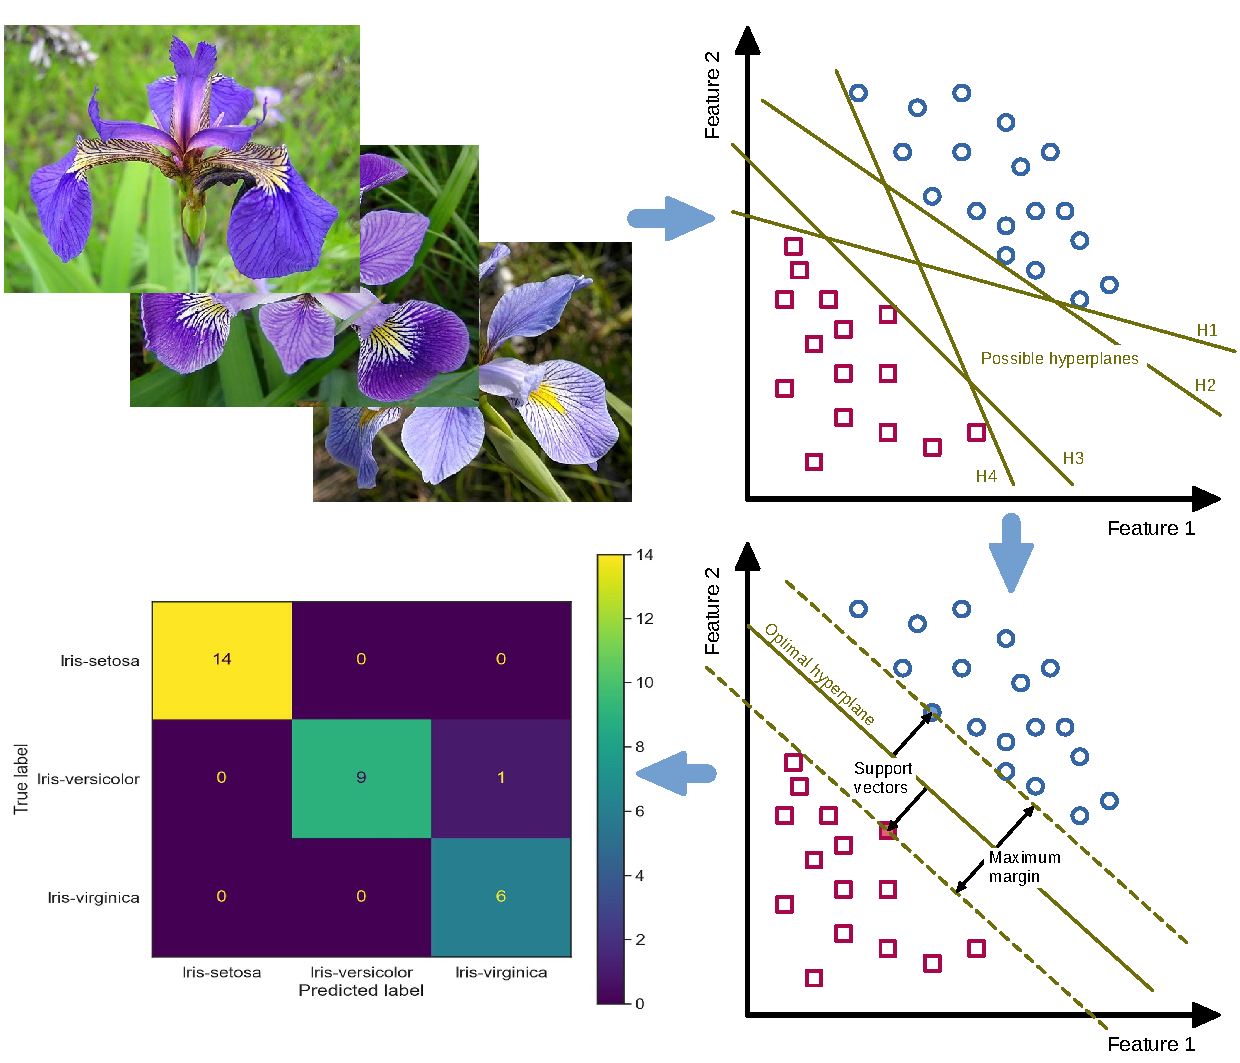
\includegraphics[width=0.90\textwidth]{images/Cover_image.pdf}
        \end{center}
        \vfill

    \begin{abstract}
    This is a placeholder for the abstract that needs to be added later.
    \end{abstract}
    \vfill

    \newpage

    % Activate own page style
    \pagestyle{fancy}
    % Delete all fields
    \fancyhf{}
    % \fancyhead[EL,OL]{$header$}
    % \fancyfoot[EL,OL]{$footer$}
    % Header leftside: chapter/section
    \fancyhead[ER,OR]{\leftmark}
    % Footer rightside: page number
    \fancyfoot[ER,OR]{Seite \thepage}

    \renewcommand{\sectionmark}[1]{
        \markboth{\thesection{} #1}{}
    }

    
    \tableofcontents
    
    


    
    \hypertarget{introduction}{%
\section{Introduction}\label{introduction}}

The \textbf{Analytic Hierarchy Process (AHP)} is a common and now widely
used method to decide on an alternative based on several different
criteria (see \cite{Wikipedia_AHP}). Often the weighting of the
respective criteria is done by a small number of decision makers or even
a single decision maker. The AHP is then relatively easy to implement,
both organizationally and technically.

Much less often, the weighting of criteria used for decision-making is
done by a variety of different stakeholders. However, especially for
decision-making with high social relevance, the involvement of many
stakeholders is very important. At this point, the following questions
arise:

\begin{enumerate}
\def\labelenumi{\arabic{enumi}.}
\tightlist
\item
  How do I collect the data?
\item
  Which software or tool can perform an AHP with data from the survey of
  a large number of stakeholders?
\item
  How can data collection and processing be combined in a way that is
  both organizationally and technically sensible and time-effective?
\end{enumerate}

As part of the DFG-funded project ``Edible Cities'', the objective was
to evaluate different forms of urban agriculture using AHP with regard
to their sustainability. The prerequisite for this was the involvement
of numerous stakeholders from various target groups in the weighting of
the previously selected criteria and sub-criteria. The pairwise
comparisons of criteria and sub-criteria required for weighting should
be performed by means of an online survey, which should ideally be
followed directly by the AHP calculation automatically. Since the
stakeholders interviewed here were predominantly people from the
non-scientific environment, the survey had to be structured to suit
these target groups.

To the authors' knowledge, the only online tool available for conducting
a survey in combination with a directly subsequent criteria weighting is
``AHP-OS'' from \href{https://bpmsg.com}{BPMSG (Business Performance
Management Singapore)}.

Reflecting the above requirements, especially with regard to the target
groups, ``AHP-OS'' appeared unsuitable, however, as it is too strongly
designed to generate consistent datasets. For this purpose, participants
are asked to reconsider their decisions several times, if necessary, and
to adjust them in the direction of consistency. This very scientific
approach would not have been appropriate for the intended target groups.

Therefore, the authors followed the approach of separating the
stakeholder survey and the subsequent weighting of the criteria in
organizational and technical terms.

This paper introduces, for the first time, a procedure in which data
collected using the online survey platform
\href{https://www.soscisurvey.de}{SoSci Survey} are subsequently
processed with the \texttt{ahpsurvey} package (see
\cite{Vignettes_ahpsurvey_2019}). This package is exclusively available
for the statistical programming language \textbf{R} and, to the authors'
knowledge, is the only tool that meets the requirements outlined in the
previous sections.

\begin{verbatim}
@TODO:
The following remains to be revised and adjusted.
\end{verbatim}

Why we use a
\href{https://en.wikipedia.org/wiki/Project_Jupyter}{Jupyter} notebook
to to publish the R program examples:

Jupyter is a new \textbf{open source} alternative to the proprietary
numerical software
\href{https://en.wikipedia.org/wiki/Wolfram_Mathematica}{Mathematica}
from \textbf{Wolfram Research} that is well on the way to become a
\textbf{standard for exchanging research results}
(\cite{Scientific_Paper_obsolete_2018};
\cite{Future_of_Research_Paper_2018}).

Originally Jupyter was intended as an IDE for the programming languages
\textbf{Julia} and \textbf{Python}. Besides that it is also possible to
install other interpreter kernels, such as the
\textbf{\href{https://irkernel.github.io/installation/}{IRkernel}} for
\textbf{R}. This can be interesting if the IDE \textbf{RStudio Desktop}
is not available on the target platform used. For example, it is very
difficult to install RStudio on the ARM-based embedded computer
\textbf{Raspberry Pi} due to many technical dependencies. In contrast,
using the R kernel in JupyterLab on the Raspberry Pi works very well and
performant.

    \hypertarget{loading-of-used-r-packages-and-definition-of-global-functions}{%
\section{Loading of used R packages and definition of global
functions}\label{loading-of-used-r-packages-and-definition-of-global-functions}}

\hypertarget{install-missing-packages-if-not-present-yet}{%
\subsection{Install missing packages if not present
yet}\label{install-missing-packages-if-not-present-yet}}

In order to load the R packages used in the next sections, they must be
installed in the R environment. The following function checks for the
presence of the packages and installs the missing ones.

\textbf{Attention:} For some R packages, several dependencies have to be
installed first using the package manager of the operating system,
e.g.~\texttt{apt\ install\ \textless{}package\ name\textgreater{}}.

In general, the use of R version \(\geq\) 4.0 is strongly recommended.
In particular, the \texttt{ahpsurvey} package, which is essential for
calculating the AHP, depends on the \texttt{randomNames} package.
However, this is only available starting with R version \(\geq\) 4.0
(refer to
\href{https://cran.r-project.org/web/packages/randomNames/index.html}{randomNames:
Generate Random Given and Surnames}).

This can be problematic especially with slightly older systems, e.g.~on
the operating system \textbf{Raspbian buster} for the very well-known
\textbf{Raspberry Pi}, R is only available in version 3.5.2. Upgrading R
in Raspbian following the instructions on
\url{https://cran.rstudio.com/bin/linux/debian/\#debian-buster-stable}
has not succeeded for the authors so far.

    \begin{tcolorbox}[breakable, size=fbox, boxrule=1pt, pad at break*=1mm,colback=cellbackground, colframe=cellborder]
\prompt{In}{incolor}{1}{\boxspacing}
\begin{Verbatim}[commandchars=\\\{\}]
\PY{c+c1}{\PYZsh{} List of R packages that are used in this script}
\PY{n}{list.of.packages}\PY{+w}{ }\PY{o}{\PYZlt{}\PYZhy{}}\PY{+w}{ }\PY{n+nf}{c}\PY{p}{(}\PY{l+s}{\PYZdq{}}\PY{l+s}{data.table\PYZdq{}}\PY{p}{,}
\PY{+w}{                      }\PY{l+s}{\PYZdq{}}\PY{l+s}{ggplot2\PYZdq{}}\PY{p}{,}
\PY{+w}{                      }\PY{l+s}{\PYZdq{}}\PY{l+s}{tidyr\PYZdq{}}\PY{p}{,}
\PY{+w}{                      }\PY{l+s}{\PYZdq{}}\PY{l+s}{dplyr\PYZdq{}}\PY{p}{,}
\PY{+w}{                      }\PY{l+s}{\PYZdq{}}\PY{l+s}{magrittr\PYZdq{}}\PY{p}{,}
\PY{+w}{                      }\PY{l+s}{\PYZdq{}}\PY{l+s}{ahpsurvey\PYZdq{}}\PY{p}{,}
\PY{+w}{                      }\PY{l+s}{\PYZdq{}}\PY{l+s}{knitr\PYZdq{}}\PY{p}{,}
\PY{+w}{                      }\PY{l+s}{\PYZdq{}}\PY{l+s}{IRdisplay\PYZdq{}}\PY{p}{,}
\PY{+w}{                      }\PY{l+s}{\PYZdq{}}\PY{l+s}{forcats\PYZdq{}}\PY{p}{)}

\PY{c+c1}{\PYZsh{} Query the already installed packages and save the missing ones in a new list}
\PY{n}{missing.packages}\PY{+w}{ }\PY{o}{\PYZlt{}\PYZhy{}}\PY{+w}{ }\PY{n}{list.of.packages}\PY{p}{[}\PY{o}{!}\PY{p}{(}\PY{n}{list.of.packages}\PY{+w}{ }
\PY{+w}{                                       }\PY{o}{\PYZpc{}in\PYZpc{}}\PY{+w}{ }\PY{n+nf}{installed.packages}\PY{p}{(}\PY{p}{)}\PY{p}{[}\PY{p}{,}\PY{l+s}{\PYZdq{}}\PY{l+s}{Package\PYZdq{}}\PY{p}{]}\PY{p}{)}\PY{p}{]}

\PY{c+c1}{\PYZsh{} Install missing packages}
\PY{n+nf}{if}\PY{p}{(}\PY{n+nf}{length}\PY{p}{(}\PY{n}{missing.packages}\PY{p}{)}\PY{p}{)}\PY{+w}{ }\PY{p}{\PYZob{}}
\PY{+w}{    }\PY{n+nf}{install.packages}\PY{p}{(}\PY{n}{missing.packages}\PY{p}{)}
\PY{p}{\PYZcb{}}\PY{+w}{ }\PY{n}{else}\PY{+w}{ }\PY{p}{\PYZob{}}
\PY{+w}{    }\PY{n+nf}{print}\PY{p}{(}\PY{l+s}{\PYZdq{}}\PY{l+s}{All required packages are installed.\PYZdq{}}\PY{p}{)}
\PY{p}{\PYZcb{}}
\end{Verbatim}
\end{tcolorbox}

    \begin{Verbatim}[commandchars=\\\{\}]
[1] "All required packages are installed."
    \end{Verbatim}

    \hypertarget{load-r-packages}{%
\subsection{Load R packages}\label{load-r-packages}}

After proving in the previous section that all required R packages are
installed, they can be loaded in the following subsections.

    \hypertarget{load-package-data.table}{%
\subsubsection{\texorpdfstring{Load package
\texttt{data.table}}{Load package data.table}}\label{load-package-data.table}}

The \texttt{data.table} package is used for \textbf{reading and editing
tables}.

\textbf{Note:} This package inherits from \texttt{data.frame}.

    \begin{tcolorbox}[breakable, size=fbox, boxrule=1pt, pad at break*=1mm,colback=cellbackground, colframe=cellborder]
\prompt{In}{incolor}{2}{\boxspacing}
\begin{Verbatim}[commandchars=\\\{\}]
\PY{n+nf}{library}\PY{p}{(}\PY{n}{data.table}\PY{p}{)}
\end{Verbatim}
\end{tcolorbox}

    \hypertarget{load-package-ggplot2}{%
\subsubsection{\texorpdfstring{Load package
\texttt{ggplot2}}{Load package ggplot2}}\label{load-package-ggplot2}}

The package \texttt{ggplot2} is used to \textbf{plot beautiful
diagrams}.

    \begin{tcolorbox}[breakable, size=fbox, boxrule=1pt, pad at break*=1mm,colback=cellbackground, colframe=cellborder]
\prompt{In}{incolor}{3}{\boxspacing}
\begin{Verbatim}[commandchars=\\\{\}]
\PY{n+nf}{library}\PY{p}{(}\PY{n}{ggplot2}\PY{p}{)}
\end{Verbatim}
\end{tcolorbox}

    \hypertarget{load-packages-knitr-and-irdisplay}{%
\subsubsection{\texorpdfstring{Load packages \texttt{knitr} and
\texttt{IRdisplay}}{Load packages knitr and IRdisplay}}\label{load-packages-knitr-and-irdisplay}}

The \texttt{kable()} function from the package \texttt{knitr} is used to
output dataframes as markdown tables.

The \texttt{display\_markdown()} function from the package
\texttt{IRdisplay} is used to \textbf{render markdown tables} in the
notebook as well as in the compiled PDF output.

    \begin{tcolorbox}[breakable, size=fbox, boxrule=1pt, pad at break*=1mm,colback=cellbackground, colframe=cellborder]
\prompt{In}{incolor}{4}{\boxspacing}
\begin{Verbatim}[commandchars=\\\{\}]
\PY{n+nf}{library}\PY{p}{(}\PY{n}{knitr}\PY{p}{)}
\PY{n+nf}{library}\PY{p}{(}\PY{n}{IRdisplay}\PY{p}{)}
\end{Verbatim}
\end{tcolorbox}

    \hypertarget{load-package-tidyr}{%
\subsubsection{\texorpdfstring{Load package
\texttt{tidyr}}{Load package tidyr}}\label{load-package-tidyr}}

The package \texttt{tidyr} is used to \textbf{reshape dataframes} and
provides functions like \texttt{gather()} or \texttt{spread()}. Some
examples for the application can be found here:
\href{https://uc-r.github.io/tidyr}{Reshaping your data with tidyr}.

    \begin{tcolorbox}[breakable, size=fbox, boxrule=1pt, pad at break*=1mm,colback=cellbackground, colframe=cellborder]
\prompt{In}{incolor}{5}{\boxspacing}
\begin{Verbatim}[commandchars=\\\{\}]
\PY{n+nf}{library}\PY{p}{(}\PY{n}{tidyr}\PY{p}{)}
\end{Verbatim}
\end{tcolorbox}

    \hypertarget{load-package-dplyr}{%
\subsubsection{\texorpdfstring{Load package
\texttt{dplyr}}{Load package dplyr}}\label{load-package-dplyr}}

The package \texttt{dplyr} is necessary to \textbf{manipulate
dataframes} using functions like \texttt{select()}, \texttt{mutate()}
and \texttt{left\_join()}.

\textbf{Hint:} Annoying messages on package loading regarding masked
functions can be suppressed by setting the parameter
\texttt{warn.conflicts=FALSE} when calling the \texttt{library()}
function.

    \begin{tcolorbox}[breakable, size=fbox, boxrule=1pt, pad at break*=1mm,colback=cellbackground, colframe=cellborder]
\prompt{In}{incolor}{6}{\boxspacing}
\begin{Verbatim}[commandchars=\\\{\}]
\PY{n+nf}{library}\PY{p}{(}\PY{n}{dplyr}\PY{p}{,}\PY{+w}{ }\PY{n}{warn.conflicts}\PY{o}{=}\PY{k+kc}{FALSE}\PY{p}{)}
\end{Verbatim}
\end{tcolorbox}

    \hypertarget{load-package-magrittr}{%
\subsubsection{\texorpdfstring{Load package
\texttt{magrittr}}{Load package magrittr}}\label{load-package-magrittr}}

The package \texttt{magrittr} provides the \textbf{pipe functionality}
and can be used to create more effective code for processing large
datasets. What pipes of the form like \texttt{\%\textgreater{}\%} are
and how to use them is described here:
\href{https://statistik-dresden.de/archives/15679}{R-Programmierung: Was
ist \texttt{\%\textgreater{}\%}?}.

\textbf{HINT:} The pipe functionality is already available by loading
the library \texttt{tidyr} - so you don't have to load it explicitly.

    \begin{tcolorbox}[breakable, size=fbox, boxrule=1pt, pad at break*=1mm,colback=cellbackground, colframe=cellborder]
\prompt{In}{incolor}{7}{\boxspacing}
\begin{Verbatim}[commandchars=\\\{\}]
\PY{n+nf}{library}\PY{p}{(}\PY{n}{magrittr}\PY{p}{,}\PY{+w}{ }\PY{n}{warn.conflicts}\PY{o}{=}\PY{k+kc}{FALSE}\PY{p}{)}
\end{Verbatim}
\end{tcolorbox}

    \hypertarget{load-package-forcats}{%
\subsubsection{\texorpdfstring{Load package
\texttt{forcats}}{Load package forcats}}\label{load-package-forcats}}

The \texttt{fct\_inorder()} function from the package \texttt{forcats}
is used to \textbf{reorder the discrete levels of diagram axes}
according to the intended order of attributes.

    \begin{tcolorbox}[breakable, size=fbox, boxrule=1pt, pad at break*=1mm,colback=cellbackground, colframe=cellborder]
\prompt{In}{incolor}{8}{\boxspacing}
\begin{Verbatim}[commandchars=\\\{\}]
\PY{n+nf}{library}\PY{p}{(}\PY{n}{forcats}\PY{p}{)}
\end{Verbatim}
\end{tcolorbox}

    \hypertarget{load-package-ahpsurvey}{%
\subsubsection{\texorpdfstring{Load package
\texttt{ahpsurvey}}{Load package ahpsurvey}}\label{load-package-ahpsurvey}}

The package \texttt{ahpsurvey} contains all the necessary mathematical
and statistical methods to run the \textbf{analytical hierarchy process
(AHP)}.

    \begin{tcolorbox}[breakable, size=fbox, boxrule=1pt, pad at break*=1mm,colback=cellbackground, colframe=cellborder]
\prompt{In}{incolor}{9}{\boxspacing}
\begin{Verbatim}[commandchars=\\\{\}]
\PY{n+nf}{library}\PY{p}{(}\PY{n}{ahpsurvey}\PY{p}{)}
\end{Verbatim}
\end{tcolorbox}

    \hypertarget{function-to-format-dataframes-as-markdown-tables}{%
\subsection{Function to format dataframes as markdown
tables}\label{function-to-format-dataframes-as-markdown-tables}}

Following function \textbf{formats given dataframes as markdown tables}
using the \texttt{kable()} function from the \texttt{knitr} package.

The \texttt{display\_markdown()} function from the package
\texttt{IRdisplay} is used to \textbf{render markdown tables} in the
notebook as well as in the compiled PDF output.

    \begin{tcolorbox}[breakable, size=fbox, boxrule=1pt, pad at break*=1mm,colback=cellbackground, colframe=cellborder]
\prompt{In}{incolor}{10}{\boxspacing}
\begin{Verbatim}[commandchars=\\\{\}]
\PY{n}{func\PYZus{}render\PYZus{}md\PYZus{}tables}\PY{+w}{ }\PY{o}{\PYZlt{}\PYZhy{}}\PY{+w}{ }\PY{n+nf}{function}\PY{p}{(}\PY{n}{df\PYZus{}table}\PY{p}{,}\PY{+w}{ }\PY{n}{str\PYZus{}table\PYZus{}header}\PY{p}{)}\PY{+w}{ }\PY{p}{\PYZob{}}
\PY{+w}{    }\PY{c+c1}{\PYZsh{} Format the dataframe as a markdown table using }
\PY{+w}{    }\PY{c+c1}{\PYZsh{} the \PYZsq{}kable()\PYZsq{} function from the \PYZsq{}knitr\PYZsq{} package.}
\PY{+w}{    }\PY{n}{table\PYZus{}out}\PY{+w}{ }\PY{o}{\PYZlt{}\PYZhy{}}\PY{+w}{ }\PY{n+nf}{kable}\PY{p}{(}
\PY{+w}{        }\PY{n}{df\PYZus{}table}\PY{p}{,}
\PY{+w}{        }\PY{n}{format}\PY{+w}{ }\PY{o}{=}\PY{+w}{ }\PY{l+s}{\PYZdq{}}\PY{l+s}{markdown\PYZdq{}}\PY{p}{,}
\PY{+w}{        }\PY{c+c1}{\PYZsh{} digits = 2,}
\PY{+w}{        }\PY{n}{caption}\PY{+w}{ }\PY{o}{=}\PY{+w}{ }\PY{n}{str\PYZus{}table\PYZus{}header}\PY{p}{)}

\PY{+w}{    }\PY{c+c1}{\PYZsh{} print(table\PYZus{}out)}
\PY{+w}{    }\PY{n+nf}{display\PYZus{}markdown}\PY{p}{(}\PY{n+nf}{as.character}\PY{p}{(}\PY{n}{table\PYZus{}out}\PY{p}{)}\PY{p}{)}
\PY{p}{\PYZcb{}}
\end{Verbatim}
\end{tcolorbox}

    \hypertarget{prepare-raw-csv-input-data-from-sosci-survey-for-analytical-hierarchy-process-ahp}{%
\section{Prepare raw CSV input data from SoSci Survey for analytical
hierarchy process
(AHP)}\label{prepare-raw-csv-input-data-from-sosci-survey-for-analytical-hierarchy-process-ahp}}

The survey was conducted on the \href{https://www.soscisurvey.de/}{SoSci
Survey} platform and the results were exported as CSV files.

In this main section the CSV files are prepared in such a way that in
the following main section the AHP can be carried out using the R
package \texttt{ahpsurvey}.

    \hypertarget{set-globally-used-input-and-output-folders-for-preparing-raw-csv-data}{%
\subsection{Set globally used input and output folders for preparing raw
CSV
data}\label{set-globally-used-input-and-output-folders-for-preparing-raw-csv-data}}

The following global variables are used to store the input and output
folders for CSV file preparation.

    \begin{tcolorbox}[breakable, size=fbox, boxrule=1pt, pad at break*=1mm,colback=cellbackground, colframe=cellborder]
\prompt{In}{incolor}{11}{\boxspacing}
\begin{Verbatim}[commandchars=\\\{\}]
\PY{n}{str\PYZus{}input\PYZus{}path\PYZus{}prep}\PY{+w}{ }\PY{o}{=}\PY{+w}{ }\PY{l+s}{\PYZdq{}}\PY{l+s}{./input\PYZus{}data\PYZus{}from\PYZus{}survey\PYZdq{}}
\PY{n}{str\PYZus{}output\PYZus{}path\PYZus{}prep}\PY{+w}{ }\PY{o}{=}\PY{+w}{ }\PY{l+s}{\PYZdq{}}\PY{l+s}{./output\PYZus{}data\PYZus{}manipulated\PYZdq{}}
\end{Verbatim}
\end{tcolorbox}

    \hypertarget{define-functions-to-prepare-the-survey-data-for-further-analysis}{%
\subsection{Define functions to prepare the survey data for further
analysis}\label{define-functions-to-prepare-the-survey-data-for-further-analysis}}

The following functions are used to read the survey data from the input
CSV files, to prepare the data structure for further analysis with the R
package \texttt{ahpsurvey} and to store the results in the output CSV
files.

\hypertarget{function-to-read-the-survey-data-from-csv-files-to-dataframe-objects}{%
\subsubsection{Function to read the survey data from CSV files to
dataframe
objects}\label{function-to-read-the-survey-data-from-csv-files-to-dataframe-objects}}

This function reads a CSV file and stores the data in four different
dataframes by selecting different columns for each. The four dataframes
contain the \textbf{main criteria}, the \textbf{environmental}, the
\textbf{social}, or the \textbf{economic sub-criteria}.

    \begin{tcolorbox}[breakable, size=fbox, boxrule=1pt, pad at break*=1mm,colback=cellbackground, colframe=cellborder]
\prompt{In}{incolor}{12}{\boxspacing}
\begin{Verbatim}[commandchars=\\\{\}]
\PY{n}{func\PYZus{}readCSVdata\PYZus{}to\PYZus{}dataframes}\PY{+w}{ }\PY{o}{\PYZlt{}\PYZhy{}}\PY{+w}{ }\PY{n+nf}{function}\PY{p}{(}\PY{n}{str\PYZus{}CSVfilename}\PY{p}{)}\PY{+w}{ }\PY{p}{\PYZob{}}
\PY{+w}{  }
\PY{+w}{  }\PY{c+c1}{\PYZsh{} Criteria (main criteria)}
\PY{+w}{  }\PY{n}{df\PYZus{}mySurvey\PYZus{}1}\PY{+w}{ }\PY{o}{\PYZlt{}\PYZhy{}}\PY{+w}{ }\PY{n+nf}{fread}\PY{p}{(}
\PY{+w}{    }\PY{n}{file}\PY{+w}{ }\PY{o}{=}\PY{+w}{ }\PY{n}{str\PYZus{}CSVfilename}\PY{p}{,}\PY{+w}{ }\PY{n}{encoding}\PY{+w}{ }\PY{o}{=}\PY{+w}{ }\PY{l+s}{\PYZdq{}}\PY{l+s}{UTF\PYZhy{}8\PYZdq{}}\PY{p}{,}
\PY{+w}{    }\PY{n}{header}\PY{+w}{ }\PY{o}{=}\PY{+w}{ }\PY{k+kc}{TRUE}\PY{p}{,}\PY{+w}{ }\PY{n}{sep}\PY{+w}{ }\PY{o}{=}\PY{+w}{ }\PY{l+s}{\PYZdq{}}\PY{l+s}{\PYZbs{}t\PYZdq{}}\PY{p}{,}\PY{+w}{ }\PY{n}{quote}\PY{+w}{ }\PY{o}{=}\PY{+w}{ }\PY{l+s}{\PYZdq{}}\PY{l+s}{\PYZbs{}\PYZdq{}\PYZdq{}}\PY{p}{,}
\PY{+w}{    }\PY{c+c1}{\PYZsh{} dec = \PYZdq{}.\PYZdq{}, row.var = \PYZdq{}CASE\PYZdq{},}
\PY{+w}{    }\PY{n}{select}\PY{+w}{ }\PY{o}{=}\PY{+w}{ }\PY{n+nf}{c}\PY{p}{(}\PY{l+s}{\PYZdq{}}\PY{l+s}{CASE\PYZdq{}}\PY{p}{,}\PY{+w}{ }\PY{l+s}{\PYZdq{}}\PY{l+s}{AK01\PYZdq{}}\PY{p}{,}\PY{+w}{ }\PY{l+s}{\PYZdq{}}\PY{l+s}{AK02\PYZdq{}}\PY{p}{,}\PY{+w}{ }\PY{l+s}{\PYZdq{}}\PY{l+s}{AK03\PYZdq{}}\PY{p}{,}
\PY{+w}{               }\PY{l+s}{\PYZdq{}}\PY{l+s}{RK01\PYZus{}01\PYZdq{}}\PY{p}{,}\PY{+w}{ }\PY{l+s}{\PYZdq{}}\PY{l+s}{RK02\PYZus{}01\PYZdq{}}\PY{p}{,}\PY{+w}{ }\PY{l+s}{\PYZdq{}}\PY{l+s}{RK03\PYZus{}01\PYZdq{}}\PY{p}{,}
\PY{+w}{               }\PY{l+s}{\PYZdq{}}\PY{l+s}{RK04\PYZus{}01\PYZdq{}}\PY{p}{,}\PY{+w}{ }\PY{l+s}{\PYZdq{}}\PY{l+s}{RK05\PYZus{}01\PYZdq{}}\PY{p}{,}\PY{+w}{ }\PY{l+s}{\PYZdq{}}\PY{l+s}{RK06\PYZus{}01\PYZdq{}}\PY{p}{)}
\PY{+w}{    }\PY{p}{)}
\PY{+w}{  }
\PY{+w}{  }\PY{c+c1}{\PYZsh{} Environmental sub\PYZhy{}criteria}
\PY{+w}{  }\PY{n}{df\PYZus{}mySurvey\PYZus{}2}\PY{+w}{ }\PY{o}{\PYZlt{}\PYZhy{}}\PY{+w}{ }\PY{n+nf}{fread}\PY{p}{(}
\PY{+w}{    }\PY{n}{file}\PY{+w}{ }\PY{o}{=}\PY{+w}{ }\PY{n}{str\PYZus{}CSVfilename}\PY{p}{,}\PY{+w}{ }\PY{n}{encoding}\PY{+w}{ }\PY{o}{=}\PY{+w}{ }\PY{l+s}{\PYZdq{}}\PY{l+s}{UTF\PYZhy{}8\PYZdq{}}\PY{p}{,}
\PY{+w}{    }\PY{n}{header}\PY{+w}{ }\PY{o}{=}\PY{+w}{ }\PY{k+kc}{TRUE}\PY{p}{,}\PY{+w}{ }\PY{n}{sep}\PY{+w}{ }\PY{o}{=}\PY{+w}{ }\PY{l+s}{\PYZdq{}}\PY{l+s}{\PYZbs{}t\PYZdq{}}\PY{p}{,}\PY{+w}{ }\PY{n}{quote}\PY{+w}{ }\PY{o}{=}\PY{+w}{ }\PY{l+s}{\PYZdq{}}\PY{l+s}{\PYZbs{}\PYZdq{}\PYZdq{}}\PY{p}{,}
\PY{+w}{    }\PY{c+c1}{\PYZsh{} dec = \PYZdq{}.\PYZdq{}, row.names = \PYZdq{}CASE\PYZdq{},}
\PY{+w}{    }\PY{n}{select}\PY{+w}{ }\PY{o}{=}\PY{+w}{ }\PY{n+nf}{c}\PY{p}{(}\PY{l+s}{\PYZdq{}}\PY{l+s}{CASE\PYZdq{}}\PY{p}{,}\PY{+w}{ }\PY{l+s}{\PYZdq{}}\PY{l+s}{AU01\PYZdq{}}\PY{p}{,}\PY{+w}{ }\PY{l+s}{\PYZdq{}}\PY{l+s}{AU02\PYZdq{}}\PY{p}{,}\PY{+w}{ }\PY{l+s}{\PYZdq{}}\PY{l+s}{AU03\PYZdq{}}\PY{p}{,}
\PY{+w}{               }\PY{l+s}{\PYZdq{}}\PY{l+s}{RU01\PYZus{}01\PYZdq{}}\PY{p}{,}\PY{+w}{ }\PY{l+s}{\PYZdq{}}\PY{l+s}{RU02\PYZus{}01\PYZdq{}}\PY{p}{,}\PY{+w}{ }\PY{l+s}{\PYZdq{}}\PY{l+s}{RU03\PYZus{}01\PYZdq{}}\PY{p}{,}
\PY{+w}{               }\PY{l+s}{\PYZdq{}}\PY{l+s}{RU04\PYZus{}01\PYZdq{}}\PY{p}{,}\PY{+w}{ }\PY{l+s}{\PYZdq{}}\PY{l+s}{RU05\PYZus{}01\PYZdq{}}\PY{p}{,}\PY{+w}{ }\PY{l+s}{\PYZdq{}}\PY{l+s}{RU06\PYZus{}01\PYZdq{}}\PY{p}{)}
\PY{+w}{    }\PY{p}{)}
\PY{+w}{  }
\PY{+w}{  }\PY{c+c1}{\PYZsh{} Social sub\PYZhy{}criteria}
\PY{+w}{  }\PY{n}{df\PYZus{}mySurvey\PYZus{}3}\PY{+w}{ }\PY{o}{\PYZlt{}\PYZhy{}}\PY{+w}{ }\PY{n+nf}{fread}\PY{p}{(}
\PY{+w}{    }\PY{n}{file}\PY{+w}{ }\PY{o}{=}\PY{+w}{ }\PY{n}{str\PYZus{}CSVfilename}\PY{p}{,}\PY{+w}{ }\PY{n}{encoding}\PY{+w}{ }\PY{o}{=}\PY{+w}{ }\PY{l+s}{\PYZdq{}}\PY{l+s}{UTF\PYZhy{}8\PYZdq{}}\PY{p}{,}
\PY{+w}{    }\PY{n}{header}\PY{+w}{ }\PY{o}{=}\PY{+w}{ }\PY{k+kc}{TRUE}\PY{p}{,}\PY{+w}{ }\PY{n}{sep}\PY{+w}{ }\PY{o}{=}\PY{+w}{ }\PY{l+s}{\PYZdq{}}\PY{l+s}{\PYZbs{}t\PYZdq{}}\PY{p}{,}\PY{+w}{ }\PY{n}{quote}\PY{+w}{ }\PY{o}{=}\PY{+w}{ }\PY{l+s}{\PYZdq{}}\PY{l+s}{\PYZbs{}\PYZdq{}\PYZdq{}}\PY{p}{,}
\PY{+w}{    }\PY{c+c1}{\PYZsh{} dec = \PYZdq{}.\PYZdq{}, row.names = \PYZdq{}CASE\PYZdq{},}
\PY{+w}{    }\PY{n}{select}\PY{+w}{ }\PY{o}{=}\PY{+w}{ }\PY{n+nf}{c}\PY{p}{(}\PY{l+s}{\PYZdq{}}\PY{l+s}{CASE\PYZdq{}}\PY{p}{,}\PY{+w}{ }\PY{l+s}{\PYZdq{}}\PY{l+s}{AS01\PYZdq{}}\PY{p}{,}\PY{+w}{ }\PY{l+s}{\PYZdq{}}\PY{l+s}{AS02\PYZdq{}}\PY{p}{,}\PY{+w}{ }\PY{l+s}{\PYZdq{}}\PY{l+s}{AS03\PYZdq{}}\PY{p}{,}
\PY{+w}{               }\PY{l+s}{\PYZdq{}}\PY{l+s}{RS01\PYZus{}01\PYZdq{}}\PY{p}{,}\PY{+w}{ }\PY{l+s}{\PYZdq{}}\PY{l+s}{RS02\PYZus{}01\PYZdq{}}\PY{p}{,}\PY{+w}{ }\PY{l+s}{\PYZdq{}}\PY{l+s}{RS03\PYZus{}01\PYZdq{}}\PY{p}{,}
\PY{+w}{               }\PY{l+s}{\PYZdq{}}\PY{l+s}{RS04\PYZus{}01\PYZdq{}}\PY{p}{,}\PY{+w}{ }\PY{l+s}{\PYZdq{}}\PY{l+s}{RS05\PYZus{}01\PYZdq{}}\PY{p}{,}\PY{+w}{ }\PY{l+s}{\PYZdq{}}\PY{l+s}{RS06\PYZus{}01\PYZdq{}}\PY{p}{)}
\PY{+w}{    }\PY{p}{)}
\PY{+w}{  }
\PY{+w}{  }\PY{c+c1}{\PYZsh{} Economic sub\PYZhy{}criteria}
\PY{+w}{  }\PY{n}{df\PYZus{}mySurvey\PYZus{}4}\PY{+w}{ }\PY{o}{\PYZlt{}\PYZhy{}}\PY{+w}{ }\PY{n+nf}{fread}\PY{p}{(}
\PY{+w}{    }\PY{n}{file}\PY{+w}{ }\PY{o}{=}\PY{+w}{ }\PY{n}{str\PYZus{}CSVfilename}\PY{p}{,}\PY{+w}{ }\PY{n}{encoding}\PY{+w}{ }\PY{o}{=}\PY{+w}{ }\PY{l+s}{\PYZdq{}}\PY{l+s}{UTF\PYZhy{}8\PYZdq{}}\PY{p}{,}
\PY{+w}{    }\PY{n}{header}\PY{+w}{ }\PY{o}{=}\PY{+w}{ }\PY{k+kc}{TRUE}\PY{p}{,}\PY{+w}{ }\PY{n}{sep}\PY{+w}{ }\PY{o}{=}\PY{+w}{ }\PY{l+s}{\PYZdq{}}\PY{l+s}{\PYZbs{}t\PYZdq{}}\PY{p}{,}\PY{+w}{ }\PY{n}{quote}\PY{+w}{ }\PY{o}{=}\PY{+w}{ }\PY{l+s}{\PYZdq{}}\PY{l+s}{\PYZbs{}\PYZdq{}\PYZdq{}}\PY{p}{,}
\PY{+w}{    }\PY{c+c1}{\PYZsh{} dec = \PYZdq{}.\PYZdq{}, row.names = \PYZdq{}CASE\PYZdq{},}
\PY{+w}{    }\PY{n}{select}\PY{+w}{ }\PY{o}{=}\PY{+w}{ }\PY{n+nf}{c}\PY{p}{(}\PY{l+s}{\PYZdq{}}\PY{l+s}{CASE\PYZdq{}}\PY{p}{,}\PY{+w}{ }\PY{l+s}{\PYZdq{}}\PY{l+s}{AW01\PYZdq{}}\PY{p}{,}\PY{+w}{ }\PY{l+s}{\PYZdq{}}\PY{l+s}{AW02\PYZdq{}}\PY{p}{,}\PY{+w}{ }\PY{l+s}{\PYZdq{}}\PY{l+s}{AW03\PYZdq{}}\PY{p}{,}
\PY{+w}{               }\PY{l+s}{\PYZdq{}}\PY{l+s}{RW01\PYZus{}01\PYZdq{}}\PY{p}{,}\PY{+w}{ }\PY{l+s}{\PYZdq{}}\PY{l+s}{RW02\PYZus{}01\PYZdq{}}\PY{p}{,}\PY{+w}{ }\PY{l+s}{\PYZdq{}}\PY{l+s}{RW03\PYZus{}01\PYZdq{}}\PY{p}{,}
\PY{+w}{               }\PY{l+s}{\PYZdq{}}\PY{l+s}{RW04\PYZus{}01\PYZdq{}}\PY{p}{,}\PY{+w}{ }\PY{l+s}{\PYZdq{}}\PY{l+s}{RW05\PYZus{}01\PYZdq{}}\PY{p}{,}\PY{+w}{ }\PY{l+s}{\PYZdq{}}\PY{l+s}{RW06\PYZus{}01\PYZdq{}}\PY{p}{)}
\PY{+w}{    }\PY{p}{)}
\PY{+w}{  }
\PY{+w}{  }\PY{n}{output}\PY{+w}{ }\PY{o}{\PYZlt{}\PYZhy{}}\PY{+w}{ }\PY{n+nf}{list}\PY{p}{(}\PY{n}{df\PYZus{}mySurvey\PYZus{}1}\PY{p}{,}\PY{+w}{ }\PY{n}{df\PYZus{}mySurvey\PYZus{}2}\PY{p}{,}\PY{+w}{ }\PY{n}{df\PYZus{}mySurvey\PYZus{}3}\PY{p}{,}\PY{+w}{ }\PY{n}{df\PYZus{}mySurvey\PYZus{}4}\PY{p}{)}
\PY{+w}{  }
\PY{+w}{  }\PY{n+nf}{return}\PY{p}{(}\PY{n}{output}\PY{p}{)}
\PY{p}{\PYZcb{}}
\end{Verbatim}
\end{tcolorbox}

    \hypertarget{function-to-adapt-the-exported-survey-data-to-saaty-scale}{%
\subsubsection{Function to adapt the exported survey data to Saaty
scale}\label{function-to-adapt-the-exported-survey-data-to-saaty-scale}}

For the \textbf{comparison of two attributes}, Saaty introduced a scale
of nine rating items shown in the following table (see
\cite{Saaty_AHP_1987}):

\begin{longtable}[]{@{}rl@{}}
\caption{Nine rating items according to Saaty (adapted from source:
\cite{Vignettes_ahpsurvey_2019})}\tabularnewline
\toprule\noalign{}
Rating & Definition \\
\midrule\noalign{}
\endfirsthead
\toprule\noalign{}
Rating & Definition \\
\midrule\noalign{}
\endhead
\bottomrule\noalign{}
\endlastfoot
1 & Two attributes are equally important \\
2 & Between 1 and 3 \\
3 & The preferred attribute is slightly more important \\
4 & Between 3 and 5 \\
5 & The preferred attribute is moderately more important \\
6 & Between 5 and 7 \\
7 & The preferred attribute is strongly more important \\
8 & Between 7 and 9 \\
9 & The preferred attribute is absolutely more important \\
\end{longtable}

To be able to describe the comparison of two attributes uniquely,
negative values as well as positive values are introduced for the rating
items. \textbf{Negative} values prefer the \(Attribute\;X\) and
\textbf{positive} values the \(Attribute\;Y\). A value of \textbf{\(1\)}
means that both attributes are \textbf{equally weighted}, i.e.~equally
important. Note that the values \(0\) and \(\text{-}1\) \textbf{do not}
exist. Thus, Saaty's 17-step scale will result as follows:

\[Attribute\;X\;\;\;\;\text{-}9\;\text{-}8\;\text{-}7\;\ldots\;\text{-}3\;\text{-}2\;\;\;\textbf{1}\;\;\;2\;3\;\ldots\;7\;8\;9\;\;\;\;Attribute\;Y\]

The package \texttt{ahpsurvey} employs the 17-step scale according to
Saaty (see \cite{Vignettes_ahpsurvey_2019}).

On the one hand, Saaty's 17-step scale was not technically well
implementable on the survey platform used
\href{https://www.soscisurvey.de/}{SoSci Survey}. On the other hand, it
had been too fine-granular for the mostly non-scientific target groups
of participants.

Therefore, a \textbf{2-stage query} was chosen as an alternative
approach. In \textbf{stage 1}, it was first asked whether, and if so,
which of the two attributes was preferred and thus given a higher
weighting. Stage 1 resulted in the following encoding:

\begin{itemize}
\tightlist
\item
  \(\text{-}1\): \(Attribute\;X\) and \(Attribute\;Y\) \textbf{equally
  important}
\item
  \(\;1\): \(Attribute\;X\) \textbf{more important} than
  \(Attribute\;Y\)
\item
  \(\;2\): \(Attribute\;X\) \textbf{less important} than
  \(Attribute\;Y\)
\end{itemize}

    With different weightings, the respondents in \textbf{stage 2} had to
decide how much more important the respective attribute was to them on a
scale of 1 to 8. Thereby, 1 corresponds to 2, 2 to 3, etc. of the rating
items according to Saaty. See the following figure:

\begin{figure}
\centering
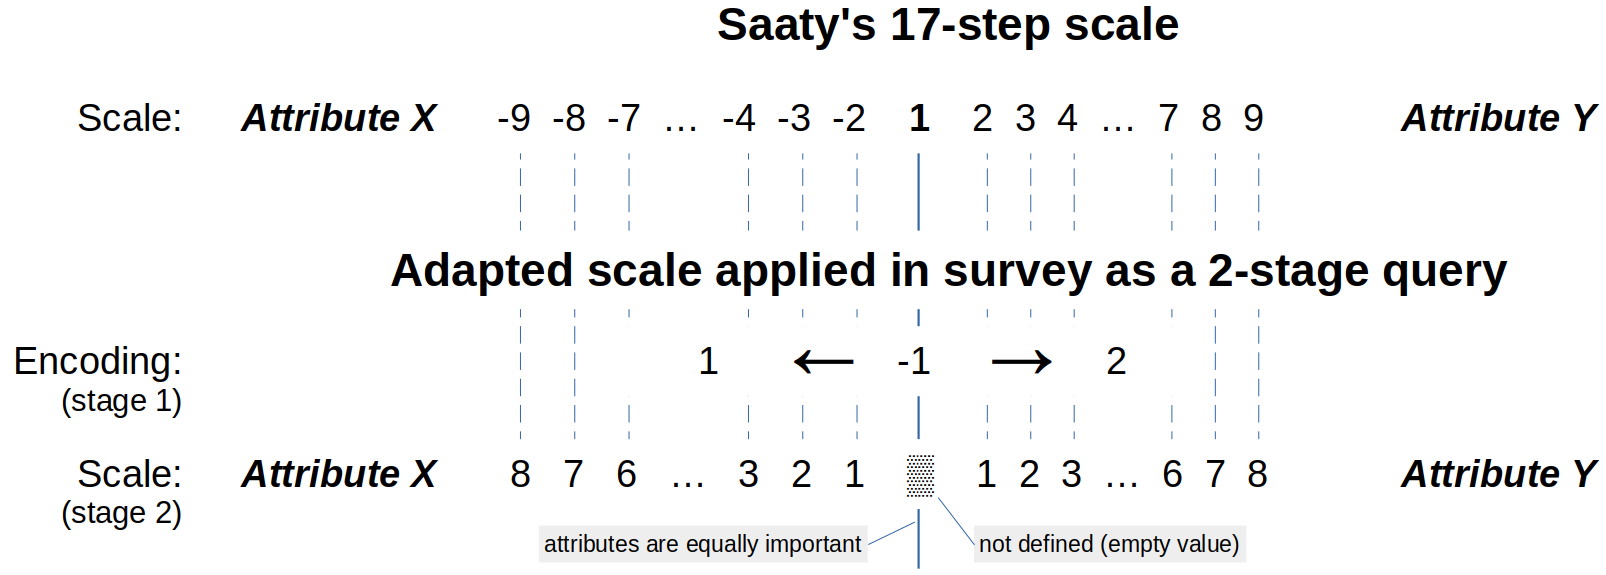
\includegraphics{images/Saaty_scale_to_SoSciSurvey.png}
\caption{Transformation from the Saaty's 17-step scale to the encoded
scale applied by a 2-stage query (source: Kasper, license: CC BY-SA
4.0)}
\end{figure}

The survey results were exported from \emph{SoSci Survey} in the form of
an \textbf{encoded scale} as a CSV file. With the following function
\texttt{func\_adaptData2SaatyScale} this now has to be converted back to
the Saaty scale in order to run AHP with the R package
\texttt{ahpsurvey}.

The values of the encoding and those of the weighting have to be taken
from the CSV file from three different columns per pairwise attribute
comparison. For example, when comparing the two attributes
``Microclimate and Hydrology (Clim)'' and ``Biodiversity (BDiv)'', the
column \texttt{AU01} contains the encoding and the columns
\texttt{RU01\_01} or \texttt{RU02\_01} the respective weighting.

The following example shows the three possible cases and the conversion
to the Saaty scale.

\textbf{Case 1:}

\begin{itemize}
\tightlist
\item
  if \texttt{AU01} \(= \text{-}1\), then set weighting \(= 1\)
\item
  attributes \texttt{Clim} and \texttt{BDiv} are equally important
\item
  values in columns \texttt{RU01\_01} or \texttt{RU02\_01} are ignored
\end{itemize}

\textbf{Case 2:}

\begin{itemize}
\tightlist
\item
  if \texttt{AU01} \(= 1\), then set weighting \(= \text{-}1\;*\)
  \texttt{RU01\_01} \(-\;1\)
\item
  the attribute \texttt{Clim} is more important than \texttt{BDiv}
\end{itemize}

\textbf{Case 3:}

\begin{itemize}
\tightlist
\item
  if \texttt{AU01} \(= 2\), then set weighting \(=\) \texttt{RU02\_01}
  \(+\;1\)
\item
  the attribute \texttt{Clim} is less important than \texttt{BDiv}
\end{itemize}

The function \texttt{func\_adaptData2SaatyScale} returns a new dataframe
with the weightings converted to the Saaty scale from three pairwise
comparisons of the criteria or sub-criterion.

    \begin{tcolorbox}[breakable, size=fbox, boxrule=1pt, pad at break*=1mm,colback=cellbackground, colframe=cellborder]
\prompt{In}{incolor}{13}{\boxspacing}
\begin{Verbatim}[commandchars=\\\{\}]
\PY{n}{func\PYZus{}adaptData2SaatyScale}\PY{+w}{ }\PY{o}{\PYZlt{}\PYZhy{}}\PY{+w}{ }\PY{n+nf}{function}\PY{p}{(}\PY{n}{df\PYZus{}inputData}\PY{p}{,}
\PY{+w}{                                      }\PY{n}{vec\PYZus{}colnames\PYZus{}search\PYZus{}1}\PY{p}{,}
\PY{+w}{                                      }\PY{n}{vec\PYZus{}colnames\PYZus{}search\PYZus{}2}\PY{p}{,}
\PY{+w}{                                      }\PY{n}{vec\PYZus{}colnames\PYZus{}out}\PY{p}{)}\PY{+w}{ }\PY{p}{\PYZob{}}
\PY{+w}{  }\PY{c+c1}{\PYZsh{} Generate new dataframe ...}
\PY{+w}{  }\PY{n}{df\PYZus{}outputData}\PY{+w}{ }\PY{o}{\PYZlt{}\PYZhy{}}\PY{+w}{ }\PY{n+nf}{data.frame}\PY{p}{(}\PY{n+nf}{matrix}\PY{p}{(}\PY{n}{ncol}\PY{+w}{ }\PY{o}{=}\PY{+w}{ }\PY{l+m}{3}\PY{p}{,}\PY{+w}{ }\PY{n}{nrow}\PY{+w}{ }\PY{o}{=}\PY{+w}{ }\PY{l+m}{0}\PY{p}{)}\PY{p}{)}
\PY{+w}{  }\PY{c+c1}{\PYZsh{} ... and name the columns}
\PY{+w}{  }\PY{n+nf}{colnames}\PY{p}{(}\PY{n}{df\PYZus{}outputData}\PY{p}{)}\PY{+w}{ }\PY{o}{\PYZlt{}\PYZhy{}}\PY{+w}{ }\PY{n}{vec\PYZus{}colnames\PYZus{}out}
\PY{+w}{  }
\PY{+w}{  }\PY{c+c1}{\PYZsh{} Generate 1. column}
\PY{+w}{  }\PY{n+nf}{for }\PY{p}{(}\PY{+w}{ }\PY{n}{row\PYZus{}idx}\PY{+w}{ }\PY{n}{in}\PY{+w}{ }\PY{l+m}{1}\PY{o}{:}\PY{n+nf}{nrow}\PY{p}{(}\PY{n}{df\PYZus{}inputData}\PY{p}{)}\PY{+w}{ }\PY{p}{)}\PY{+w}{ }\PY{p}{\PYZob{}}
\PY{+w}{    }\PY{c+c1}{\PYZsh{} Filter column names by vector element}
\PY{+w}{    }\PY{n+nf}{if }\PY{p}{(}\PY{n}{df\PYZus{}inputData}\PY{p}{[}\PY{n}{row\PYZus{}idx}\PY{p}{,}\PY{+w}{ }\PY{n+nf}{colnames}\PY{p}{(}\PY{n}{df\PYZus{}inputData}\PY{p}{)}
\PY{+w}{        }\PY{o}{\PYZpc{}in\PYZpc{}}\PY{+w}{ }\PY{n}{vec\PYZus{}colnames\PYZus{}search\PYZus{}1}\PY{p}{[}\PY{l+m}{1}\PY{p}{]}\PY{p}{,}\PY{+w}{ }\PY{n}{with}\PY{o}{=}\PY{k+kc}{FALSE}\PY{p}{]}\PY{+w}{ }\PY{o}{==}\PY{+w}{ }\PY{l+m}{1}\PY{p}{)}\PY{+w}{ }\PY{p}{\PYZob{}}
\PY{+w}{      }\PY{n}{int\PYZus{}tmp\PYZus{}val}\PY{+w}{ }\PY{o}{\PYZlt{}\PYZhy{}}\PY{+w}{ }\PY{n+nf}{as.integer}\PY{p}{(}\PY{n}{df\PYZus{}inputData}\PY{p}{[}\PY{n}{row\PYZus{}idx}\PY{p}{,}\PY{+w}{ }\PY{n+nf}{colnames}\PY{p}{(}\PY{n}{df\PYZus{}inputData}\PY{p}{)}
\PY{+w}{                     }\PY{o}{\PYZpc{}in\PYZpc{}}\PY{+w}{ }\PY{n}{vec\PYZus{}colnames\PYZus{}search\PYZus{}2}\PY{p}{[}\PY{l+m}{1}\PY{p}{]}\PY{p}{,}\PY{+w}{ }\PY{n}{with}\PY{o}{=}\PY{k+kc}{FALSE}\PY{p}{]}\PY{p}{)}
\PY{+w}{      }\PY{n}{int\PYZus{}tmp\PYZus{}val}\PY{+w}{ }\PY{o}{\PYZlt{}\PYZhy{}}\PY{+w}{ }\PY{n}{int\PYZus{}tmp\PYZus{}val}\PY{+w}{ }\PY{o}{*}\PY{+w}{ }\PY{l+m}{\PYZhy{}1}\PY{+w}{ }\PY{o}{\PYZhy{}}\PY{+w}{ }\PY{l+m}{1}

\PY{+w}{      }\PY{n}{df\PYZus{}outputData}\PY{p}{[}\PY{n}{row\PYZus{}idx}\PY{p}{,}\PY{+w}{ }\PY{n}{vec\PYZus{}colnames\PYZus{}out}\PY{p}{[}\PY{l+m}{1}\PY{p}{]]}\PY{+w}{ }\PY{o}{\PYZlt{}\PYZhy{}}\PY{+w}{ }\PY{n}{int\PYZus{}tmp\PYZus{}val}
\PY{+w}{    }\PY{p}{\PYZcb{}}
\PY{+w}{    }\PY{n}{else}\PY{+w}{ }\PY{n+nf}{if }\PY{p}{(}\PY{n}{df\PYZus{}inputData}\PY{p}{[}\PY{n}{row\PYZus{}idx}\PY{p}{,}\PY{+w}{ }\PY{n+nf}{colnames}\PY{p}{(}\PY{n}{df\PYZus{}inputData}\PY{p}{)}
\PY{+w}{             }\PY{o}{\PYZpc{}in\PYZpc{}}\PY{+w}{ }\PY{n}{vec\PYZus{}colnames\PYZus{}search\PYZus{}1}\PY{p}{[}\PY{l+m}{1}\PY{p}{]}\PY{p}{,}\PY{+w}{ }\PY{n}{with}\PY{o}{=}\PY{k+kc}{FALSE}\PY{p}{]}\PY{+w}{ }\PY{o}{==}\PY{+w}{ }\PY{l+m}{\PYZhy{}1}\PY{p}{)}\PY{+w}{ }\PY{p}{\PYZob{}}
\PY{+w}{      }\PY{n}{df\PYZus{}outputData}\PY{p}{[}\PY{n}{row\PYZus{}idx}\PY{p}{,}\PY{+w}{ }\PY{n}{vec\PYZus{}colnames\PYZus{}out}\PY{p}{[}\PY{l+m}{1}\PY{p}{]]}\PY{+w}{ }\PY{o}{\PYZlt{}\PYZhy{}}\PY{+w}{ }\PY{l+m}{1}
\PY{+w}{    }\PY{p}{\PYZcb{}}
\PY{+w}{    }\PY{n}{else}\PY{+w}{ }\PY{n+nf}{if }\PY{p}{(}\PY{n}{df\PYZus{}inputData}\PY{p}{[}\PY{n}{row\PYZus{}idx}\PY{p}{,}\PY{+w}{ }\PY{n+nf}{colnames}\PY{p}{(}\PY{n}{df\PYZus{}inputData}\PY{p}{)}
\PY{+w}{             }\PY{o}{\PYZpc{}in\PYZpc{}}\PY{+w}{ }\PY{n}{vec\PYZus{}colnames\PYZus{}search\PYZus{}1}\PY{p}{[}\PY{l+m}{1}\PY{p}{]}\PY{p}{,}\PY{+w}{ }\PY{n}{with}\PY{o}{=}\PY{k+kc}{FALSE}\PY{p}{]}\PY{+w}{ }\PY{o}{==}\PY{+w}{ }\PY{l+m}{2}\PY{p}{)}\PY{+w}{ }\PY{p}{\PYZob{}}
\PY{+w}{      }\PY{n}{int\PYZus{}tmp\PYZus{}val}\PY{+w}{ }\PY{o}{\PYZlt{}\PYZhy{}}\PY{+w}{ }\PY{n+nf}{as.integer}\PY{p}{(}\PY{n}{df\PYZus{}inputData}\PY{p}{[}\PY{n}{row\PYZus{}idx}\PY{p}{,}\PY{+w}{ }\PY{n+nf}{colnames}\PY{p}{(}\PY{n}{df\PYZus{}inputData}\PY{p}{)}
\PY{+w}{                     }\PY{o}{\PYZpc{}in\PYZpc{}}\PY{+w}{ }\PY{n}{vec\PYZus{}colnames\PYZus{}search\PYZus{}2}\PY{p}{[}\PY{l+m}{2}\PY{p}{]}\PY{p}{,}\PY{+w}{ }\PY{n}{with}\PY{o}{=}\PY{k+kc}{FALSE}\PY{p}{]}\PY{p}{)}
\PY{+w}{      }\PY{n}{int\PYZus{}tmp\PYZus{}val}\PY{+w}{ }\PY{o}{\PYZlt{}\PYZhy{}}\PY{+w}{ }\PY{n}{int\PYZus{}tmp\PYZus{}val}\PY{+w}{ }\PY{o}{+}\PY{+w}{ }\PY{l+m}{1}

\PY{+w}{      }\PY{n}{df\PYZus{}outputData}\PY{p}{[}\PY{n}{row\PYZus{}idx}\PY{p}{,}\PY{+w}{ }\PY{n}{vec\PYZus{}colnames\PYZus{}out}\PY{p}{[}\PY{l+m}{1}\PY{p}{]]}\PY{+w}{ }\PY{o}{\PYZlt{}\PYZhy{}}\PY{+w}{ }\PY{n}{int\PYZus{}tmp\PYZus{}val}
\PY{+w}{    }\PY{p}{\PYZcb{}}
\PY{+w}{  }\PY{p}{\PYZcb{}}
\PY{+w}{  }
\PY{+w}{  }\PY{c+c1}{\PYZsh{} Generate 2. column}
\PY{+w}{  }\PY{n+nf}{for }\PY{p}{(}\PY{+w}{ }\PY{n}{row\PYZus{}idx}\PY{+w}{ }\PY{n}{in}\PY{+w}{ }\PY{l+m}{1}\PY{o}{:}\PY{n+nf}{nrow}\PY{p}{(}\PY{n}{df\PYZus{}inputData}\PY{p}{)}\PY{+w}{ }\PY{p}{)}\PY{+w}{ }\PY{p}{\PYZob{}}
\PY{+w}{    }\PY{c+c1}{\PYZsh{} Filter column names by vector element}
\PY{+w}{    }\PY{n+nf}{if }\PY{p}{(}\PY{n}{df\PYZus{}inputData}\PY{p}{[}\PY{n}{row\PYZus{}idx}\PY{p}{,}\PY{+w}{ }\PY{n+nf}{colnames}\PY{p}{(}\PY{n}{df\PYZus{}inputData}\PY{p}{)}
\PY{+w}{        }\PY{o}{\PYZpc{}in\PYZpc{}}\PY{+w}{ }\PY{n}{vec\PYZus{}colnames\PYZus{}search\PYZus{}1}\PY{p}{[}\PY{l+m}{2}\PY{p}{]}\PY{p}{,}\PY{+w}{ }\PY{n}{with}\PY{o}{=}\PY{k+kc}{FALSE}\PY{p}{]}\PY{+w}{ }\PY{o}{==}\PY{+w}{ }\PY{l+m}{1}\PY{p}{)}\PY{+w}{ }\PY{p}{\PYZob{}}
\PY{+w}{      }\PY{n}{int\PYZus{}tmp\PYZus{}val}\PY{+w}{ }\PY{o}{\PYZlt{}\PYZhy{}}\PY{+w}{ }\PY{n+nf}{as.integer}\PY{p}{(}\PY{n}{df\PYZus{}inputData}\PY{p}{[}\PY{n}{row\PYZus{}idx}\PY{p}{,}\PY{+w}{ }\PY{n+nf}{colnames}\PY{p}{(}\PY{n}{df\PYZus{}inputData}\PY{p}{)}
\PY{+w}{                     }\PY{o}{\PYZpc{}in\PYZpc{}}\PY{+w}{ }\PY{n}{vec\PYZus{}colnames\PYZus{}search\PYZus{}2}\PY{p}{[}\PY{l+m}{3}\PY{p}{]}\PY{p}{,}\PY{+w}{ }\PY{n}{with}\PY{o}{=}\PY{k+kc}{FALSE}\PY{p}{]}\PY{p}{)}
\PY{+w}{      }\PY{n}{int\PYZus{}tmp\PYZus{}val}\PY{+w}{ }\PY{o}{\PYZlt{}\PYZhy{}}\PY{+w}{ }\PY{n}{int\PYZus{}tmp\PYZus{}val}\PY{+w}{ }\PY{o}{*}\PY{+w}{ }\PY{l+m}{\PYZhy{}1}\PY{+w}{ }\PY{o}{\PYZhy{}}\PY{+w}{ }\PY{l+m}{1}
\PY{+w}{      }
\PY{+w}{      }\PY{n}{df\PYZus{}outputData}\PY{p}{[}\PY{n}{row\PYZus{}idx}\PY{p}{,}\PY{+w}{ }\PY{n}{vec\PYZus{}colnames\PYZus{}out}\PY{p}{[}\PY{l+m}{2}\PY{p}{]]}\PY{+w}{ }\PY{o}{\PYZlt{}\PYZhy{}}\PY{+w}{ }\PY{n}{int\PYZus{}tmp\PYZus{}val}
\PY{+w}{    }\PY{p}{\PYZcb{}}\PY{+w}{ }
\PY{+w}{    }\PY{n}{else}\PY{+w}{ }\PY{n+nf}{if }\PY{p}{(}\PY{n}{df\PYZus{}inputData}\PY{p}{[}\PY{n}{row\PYZus{}idx}\PY{p}{,}\PY{+w}{ }\PY{n+nf}{colnames}\PY{p}{(}\PY{n}{df\PYZus{}inputData}\PY{p}{)}
\PY{+w}{             }\PY{o}{\PYZpc{}in\PYZpc{}}\PY{+w}{ }\PY{n}{vec\PYZus{}colnames\PYZus{}search\PYZus{}1}\PY{p}{[}\PY{l+m}{2}\PY{p}{]}\PY{p}{,}\PY{+w}{ }\PY{n}{with}\PY{o}{=}\PY{k+kc}{FALSE}\PY{p}{]}\PY{+w}{ }\PY{o}{==}\PY{+w}{ }\PY{l+m}{\PYZhy{}1}\PY{p}{)}\PY{+w}{ }\PY{p}{\PYZob{}}
\PY{+w}{      }\PY{n}{df\PYZus{}outputData}\PY{p}{[}\PY{n}{row\PYZus{}idx}\PY{p}{,}\PY{+w}{ }\PY{n}{vec\PYZus{}colnames\PYZus{}out}\PY{p}{[}\PY{l+m}{2}\PY{p}{]]}\PY{+w}{ }\PY{o}{\PYZlt{}\PYZhy{}}\PY{+w}{ }\PY{l+m}{1}
\PY{+w}{    }\PY{p}{\PYZcb{}}\PY{+w}{ }
\PY{+w}{    }\PY{n}{else}\PY{+w}{ }\PY{n+nf}{if }\PY{p}{(}\PY{n}{df\PYZus{}inputData}\PY{p}{[}\PY{n}{row\PYZus{}idx}\PY{p}{,}\PY{+w}{ }\PY{n+nf}{colnames}\PY{p}{(}\PY{n}{df\PYZus{}inputData}\PY{p}{)}
\PY{+w}{             }\PY{o}{\PYZpc{}in\PYZpc{}}\PY{+w}{ }\PY{n}{vec\PYZus{}colnames\PYZus{}search\PYZus{}1}\PY{p}{[}\PY{l+m}{2}\PY{p}{]}\PY{p}{,}\PY{+w}{ }\PY{n}{with}\PY{o}{=}\PY{k+kc}{FALSE}\PY{p}{]}\PY{+w}{ }\PY{o}{==}\PY{+w}{ }\PY{l+m}{2}\PY{p}{)}\PY{+w}{ }\PY{p}{\PYZob{}}
\PY{+w}{      }\PY{n}{int\PYZus{}tmp\PYZus{}val}\PY{+w}{ }\PY{o}{\PYZlt{}\PYZhy{}}\PY{+w}{ }\PY{n+nf}{as.integer}\PY{p}{(}\PY{n}{df\PYZus{}inputData}\PY{p}{[}\PY{n}{row\PYZus{}idx}\PY{p}{,}\PY{+w}{ }\PY{n+nf}{colnames}\PY{p}{(}\PY{n}{df\PYZus{}inputData}\PY{p}{)}
\PY{+w}{                     }\PY{o}{\PYZpc{}in\PYZpc{}}\PY{+w}{ }\PY{n}{vec\PYZus{}colnames\PYZus{}search\PYZus{}2}\PY{p}{[}\PY{l+m}{4}\PY{p}{]}\PY{p}{,}\PY{+w}{ }\PY{n}{with}\PY{o}{=}\PY{k+kc}{FALSE}\PY{p}{]}\PY{p}{)}
\PY{+w}{      }\PY{n}{int\PYZus{}tmp\PYZus{}val}\PY{+w}{ }\PY{o}{\PYZlt{}\PYZhy{}}\PY{+w}{ }\PY{n}{int\PYZus{}tmp\PYZus{}val}\PY{+w}{ }\PY{o}{+}\PY{+w}{ }\PY{l+m}{1}
\PY{+w}{      }
\PY{+w}{      }\PY{n}{df\PYZus{}outputData}\PY{p}{[}\PY{n}{row\PYZus{}idx}\PY{p}{,}\PY{+w}{ }\PY{n}{vec\PYZus{}colnames\PYZus{}out}\PY{p}{[}\PY{l+m}{2}\PY{p}{]]}\PY{+w}{ }\PY{o}{\PYZlt{}\PYZhy{}}\PY{+w}{ }\PY{n}{int\PYZus{}tmp\PYZus{}val}
\PY{+w}{    }\PY{p}{\PYZcb{}}
\PY{+w}{  }\PY{p}{\PYZcb{}}
\PY{+w}{  }
\PY{+w}{  }\PY{c+c1}{\PYZsh{} Generate 3. column}
\PY{+w}{  }\PY{n+nf}{for }\PY{p}{(}\PY{+w}{ }\PY{n}{row\PYZus{}idx}\PY{+w}{ }\PY{n}{in}\PY{+w}{ }\PY{l+m}{1}\PY{o}{:}\PY{n+nf}{nrow}\PY{p}{(}\PY{n}{df\PYZus{}inputData}\PY{p}{)}\PY{+w}{ }\PY{p}{)}\PY{+w}{ }\PY{p}{\PYZob{}}
\PY{+w}{    }\PY{c+c1}{\PYZsh{} Filter column names by vector element}
\PY{+w}{    }\PY{n+nf}{if }\PY{p}{(}\PY{n}{df\PYZus{}inputData}\PY{p}{[}\PY{n}{row\PYZus{}idx}\PY{p}{,}\PY{+w}{ }\PY{n+nf}{colnames}\PY{p}{(}\PY{n}{df\PYZus{}inputData}\PY{p}{)}
\PY{+w}{        }\PY{o}{\PYZpc{}in\PYZpc{}}\PY{+w}{ }\PY{n}{vec\PYZus{}colnames\PYZus{}search\PYZus{}1}\PY{p}{[}\PY{l+m}{3}\PY{p}{]}\PY{p}{,}\PY{+w}{ }\PY{n}{with}\PY{o}{=}\PY{k+kc}{FALSE}\PY{p}{]}\PY{+w}{ }\PY{o}{==}\PY{+w}{ }\PY{l+m}{1}\PY{p}{)}\PY{+w}{ }\PY{p}{\PYZob{}}
\PY{+w}{      }\PY{n}{int\PYZus{}tmp\PYZus{}val}\PY{+w}{ }\PY{o}{\PYZlt{}\PYZhy{}}\PY{+w}{ }\PY{n+nf}{as.integer}\PY{p}{(}\PY{n}{df\PYZus{}inputData}\PY{p}{[}\PY{n}{row\PYZus{}idx}\PY{p}{,}\PY{+w}{ }\PY{n+nf}{colnames}\PY{p}{(}\PY{n}{df\PYZus{}inputData}\PY{p}{)}
\PY{+w}{                     }\PY{o}{\PYZpc{}in\PYZpc{}}\PY{+w}{ }\PY{n}{vec\PYZus{}colnames\PYZus{}search\PYZus{}2}\PY{p}{[}\PY{l+m}{5}\PY{p}{]}\PY{p}{,}\PY{+w}{ }\PY{n}{with}\PY{o}{=}\PY{k+kc}{FALSE}\PY{p}{]}\PY{p}{)}
\PY{+w}{      }\PY{n}{int\PYZus{}tmp\PYZus{}val}\PY{+w}{ }\PY{o}{\PYZlt{}\PYZhy{}}\PY{+w}{ }\PY{n}{int\PYZus{}tmp\PYZus{}val}\PY{+w}{ }\PY{o}{*}\PY{+w}{ }\PY{l+m}{\PYZhy{}1}\PY{+w}{ }\PY{o}{\PYZhy{}}\PY{+w}{ }\PY{l+m}{1}
\PY{+w}{      }
\PY{+w}{      }\PY{n}{df\PYZus{}outputData}\PY{p}{[}\PY{n}{row\PYZus{}idx}\PY{p}{,}\PY{+w}{ }\PY{n}{vec\PYZus{}colnames\PYZus{}out}\PY{p}{[}\PY{l+m}{3}\PY{p}{]]}\PY{+w}{ }\PY{o}{\PYZlt{}\PYZhy{}}\PY{+w}{ }\PY{n}{int\PYZus{}tmp\PYZus{}val}
\PY{+w}{    }\PY{p}{\PYZcb{}}\PY{+w}{ }
\PY{+w}{    }\PY{n}{else}\PY{+w}{ }\PY{n+nf}{if }\PY{p}{(}\PY{n}{df\PYZus{}inputData}\PY{p}{[}\PY{n}{row\PYZus{}idx}\PY{p}{,}\PY{+w}{ }\PY{n+nf}{colnames}\PY{p}{(}\PY{n}{df\PYZus{}inputData}\PY{p}{)}
\PY{+w}{             }\PY{o}{\PYZpc{}in\PYZpc{}}\PY{+w}{ }\PY{n}{vec\PYZus{}colnames\PYZus{}search\PYZus{}1}\PY{p}{[}\PY{l+m}{3}\PY{p}{]}\PY{p}{,}\PY{+w}{ }\PY{n}{with}\PY{o}{=}\PY{k+kc}{FALSE}\PY{p}{]}\PY{+w}{ }\PY{o}{==}\PY{+w}{ }\PY{l+m}{\PYZhy{}1}\PY{p}{)}\PY{+w}{ }\PY{p}{\PYZob{}}
\PY{+w}{      }\PY{n}{df\PYZus{}outputData}\PY{p}{[}\PY{n}{row\PYZus{}idx}\PY{p}{,}\PY{+w}{ }\PY{n}{vec\PYZus{}colnames\PYZus{}out}\PY{p}{[}\PY{l+m}{3}\PY{p}{]]}\PY{+w}{ }\PY{o}{\PYZlt{}\PYZhy{}}\PY{+w}{ }\PY{l+m}{1}
\PY{+w}{    }\PY{p}{\PYZcb{}}\PY{+w}{ }
\PY{+w}{    }\PY{n}{else}\PY{+w}{ }\PY{n+nf}{if }\PY{p}{(}\PY{n}{df\PYZus{}inputData}\PY{p}{[}\PY{n}{row\PYZus{}idx}\PY{p}{,}\PY{+w}{ }\PY{n+nf}{colnames}\PY{p}{(}\PY{n}{df\PYZus{}inputData}\PY{p}{)}
\PY{+w}{             }\PY{o}{\PYZpc{}in\PYZpc{}}\PY{+w}{ }\PY{n}{vec\PYZus{}colnames\PYZus{}search\PYZus{}1}\PY{p}{[}\PY{l+m}{3}\PY{p}{]}\PY{p}{,}\PY{+w}{ }\PY{n}{with}\PY{o}{=}\PY{k+kc}{FALSE}\PY{p}{]}\PY{+w}{ }\PY{o}{==}\PY{+w}{ }\PY{l+m}{2}\PY{p}{)}\PY{+w}{ }\PY{p}{\PYZob{}}
\PY{+w}{      }\PY{n}{int\PYZus{}tmp\PYZus{}val}\PY{+w}{ }\PY{o}{\PYZlt{}\PYZhy{}}\PY{+w}{ }\PY{n+nf}{as.integer}\PY{p}{(}\PY{n}{df\PYZus{}inputData}\PY{p}{[}\PY{n}{row\PYZus{}idx}\PY{p}{,}\PY{+w}{ }\PY{n+nf}{colnames}\PY{p}{(}\PY{n}{df\PYZus{}inputData}\PY{p}{)}
\PY{+w}{                     }\PY{o}{\PYZpc{}in\PYZpc{}}\PY{+w}{ }\PY{n}{vec\PYZus{}colnames\PYZus{}search\PYZus{}2}\PY{p}{[}\PY{l+m}{6}\PY{p}{]}\PY{p}{,}\PY{+w}{ }\PY{n}{with}\PY{o}{=}\PY{k+kc}{FALSE}\PY{p}{]}\PY{p}{)}
\PY{+w}{      }\PY{n}{int\PYZus{}tmp\PYZus{}val}\PY{+w}{ }\PY{o}{\PYZlt{}\PYZhy{}}\PY{+w}{ }\PY{n}{int\PYZus{}tmp\PYZus{}val}\PY{+w}{ }\PY{o}{+}\PY{+w}{ }\PY{l+m}{1}
\PY{+w}{      }
\PY{+w}{      }\PY{n}{df\PYZus{}outputData}\PY{p}{[}\PY{n}{row\PYZus{}idx}\PY{p}{,}\PY{+w}{ }\PY{n}{vec\PYZus{}colnames\PYZus{}out}\PY{p}{[}\PY{l+m}{3}\PY{p}{]]}\PY{+w}{ }\PY{o}{\PYZlt{}\PYZhy{}}\PY{+w}{ }\PY{n}{int\PYZus{}tmp\PYZus{}val}
\PY{+w}{    }\PY{p}{\PYZcb{}}
\PY{+w}{  }\PY{p}{\PYZcb{}}
\PY{+w}{  }
\PY{+w}{  }\PY{c+c1}{\PYZsh{} Return rescaled dataframe}
\PY{+w}{  }\PY{n+nf}{return}\PY{p}{(}\PY{n}{df\PYZus{}outputData}\PY{p}{)}
\PY{p}{\PYZcb{}}
\end{Verbatim}
\end{tcolorbox}

    \hypertarget{function-to-write-resulting-dataframes-to-csv-files}{%
\subsubsection{Function to write resulting dataframes to CSV
files}\label{function-to-write-resulting-dataframes-to-csv-files}}

With this function, the results of the data preparation are saved in
output CSV files.

    \begin{tcolorbox}[breakable, size=fbox, boxrule=1pt, pad at break*=1mm,colback=cellbackground, colframe=cellborder]
\prompt{In}{incolor}{14}{\boxspacing}
\begin{Verbatim}[commandchars=\\\{\}]
\PY{n}{func\PYZus{}writeDataframe\PYZus{}to\PYZus{}CSVfile}\PY{+w}{ }\PY{o}{\PYZlt{}\PYZhy{}}\PY{+w}{ }\PY{n+nf}{function}\PY{p}{(}\PY{n}{str\PYZus{}path}\PY{p}{,}\PY{+w}{ }\PY{n}{str\PYZus{}CSVfilename}\PY{p}{,}
\PY{+w}{                                           }\PY{n}{df\PYZus{}dataframe}\PY{p}{,}\PY{+w}{ }\PY{n}{str\PYZus{}filenameExtension}\PY{p}{)}\PY{+w}{ }\PY{p}{\PYZob{}}
\PY{+w}{  }\PY{c+c1}{\PYZsh{} How to split the file name on second underscore,}
\PY{+w}{  }\PY{c+c1}{\PYZsh{} was found here: https://stackoverflow.com/a/32398489}
\PY{+w}{  }\PY{n}{list\PYZus{}str\PYZus{}split}\PY{+w}{ }\PY{o}{\PYZlt{}\PYZhy{}}\PY{+w}{ }\PY{n+nf}{strsplit}\PY{p}{(}\PY{n+nf}{sub}\PY{p}{(}\PY{l+s}{\PYZsq{}}\PY{l+s}{(\PYZca{}[\PYZca{}\PYZus{}]+\PYZus{}[\PYZca{}\PYZus{}]+)\PYZus{}(.*)\PYZdl{}\PYZsq{}}\PY{p}{,}\PY{+w}{ }\PY{l+s}{\PYZsq{}}\PY{l+s}{\PYZbs{}\PYZbs{}1 \PYZbs{}\PYZbs{}2\PYZsq{}}\PY{p}{,}
\PY{+w}{                                 }\PY{n}{str\PYZus{}CSVfilename}\PY{p}{)}\PY{p}{,}\PY{+w}{ }\PY{l+s}{\PYZsq{}}\PY{l+s}{ \PYZsq{}}\PY{p}{)}
\PY{+w}{  }
\PY{+w}{  }\PY{c+c1}{\PYZsh{} Extend the file name prefix and glue together with old suffix}
\PY{+w}{  }\PY{n}{str\PYZus{}CSVfilename\PYZus{}extended}\PY{+w}{ }\PY{o}{\PYZlt{}\PYZhy{}}\PY{+w}{ }\PY{n+nf}{paste}\PY{p}{(}\PY{n}{list\PYZus{}str\PYZus{}split}\PY{p}{[[}\PY{l+m}{1}\PY{p}{]]}\PY{p}{[}\PY{l+m}{1}\PY{p}{]}\PY{p}{,}
\PY{+w}{                                    }\PY{n}{str\PYZus{}filenameExtension}\PY{p}{,}
\PY{+w}{                                    }\PY{n}{list\PYZus{}str\PYZus{}split}\PY{p}{[[}\PY{l+m}{1}\PY{p}{]]}\PY{p}{[}\PY{l+m}{2}\PY{p}{]}\PY{p}{,}\PY{+w}{ }\PY{n}{sep}\PY{o}{=}\PY{l+s}{\PYZdq{}}\PY{l+s}{\PYZus{}\PYZdq{}}\PY{p}{)}
\PY{+w}{  }
\PY{+w}{  }\PY{c+c1}{\PYZsh{} Extend file name by path}
\PY{+w}{  }\PY{n}{str\PYZus{}CSVfilename\PYZus{}extended}\PY{+w}{ }\PY{o}{\PYZlt{}\PYZhy{}}\PY{+w}{ }\PY{n+nf}{paste}\PY{p}{(}\PY{n}{str\PYZus{}path}\PY{p}{,}\PY{+w}{ }\PY{n}{str\PYZus{}CSVfilename\PYZus{}extended}\PY{p}{,}\PY{+w}{ }\PY{n}{sep}\PY{o}{=}\PY{l+s}{\PYZdq{}}\PY{l+s}{/\PYZdq{}}\PY{p}{)}
\PY{+w}{  }
\PY{+w}{  }\PY{n+nf}{write.table}\PY{p}{(}\PY{n}{df\PYZus{}dataframe}\PY{p}{,}\PY{+w}{ }\PY{n}{file}\PY{+w}{ }\PY{o}{=}\PY{+w}{ }\PY{n}{str\PYZus{}CSVfilename\PYZus{}extended}\PY{p}{,}
\PY{+w}{              }\PY{n}{fileEncoding}\PY{+w}{ }\PY{o}{=}\PY{+w}{ }\PY{l+s}{\PYZdq{}}\PY{l+s}{UTF\PYZhy{}8\PYZdq{}}\PY{p}{,}\PY{+w}{ }\PY{n}{row.names}\PY{+w}{ }\PY{o}{=}\PY{+w}{ }\PY{k+kc}{FALSE}\PY{p}{,}
\PY{+w}{              }\PY{n}{col.names}\PY{+w}{ }\PY{o}{=}\PY{+w}{ }\PY{k+kc}{TRUE}\PY{p}{,}\PY{+w}{ }\PY{n}{sep}\PY{+w}{ }\PY{o}{=}\PY{+w}{ }\PY{l+s}{\PYZdq{}}\PY{l+s}{\PYZbs{}t\PYZdq{}}\PY{p}{,}\PY{+w}{ }\PY{n}{quote}\PY{+w}{ }\PY{o}{=}\PY{+w}{ }\PY{k+kc}{TRUE}\PY{p}{)}
\PY{p}{\PYZcb{}}
\end{Verbatim}
\end{tcolorbox}

    \hypertarget{create-dataframe-handling-the-file-names-of-input-csv-data-raw-data-from-survey}{%
\subsection{Create dataframe handling the file names of input CSV data
(raw data from
survey)}\label{create-dataframe-handling-the-file-names-of-input-csv-data-raw-data-from-survey}}

    \begin{tcolorbox}[breakable, size=fbox, boxrule=1pt, pad at break*=1mm,colback=cellbackground, colframe=cellborder]
\prompt{In}{incolor}{15}{\boxspacing}
\begin{Verbatim}[commandchars=\\\{\}]
\PY{n}{df\PYZus{}csvInputFiles}\PY{+w}{ }\PY{o}{\PYZlt{}\PYZhy{}}\PY{+w}{ }\PY{n+nf}{data.table}\PY{p}{(}
\PY{+w}{  }\PY{n}{file\PYZus{}idx}\PY{+w}{ }\PY{o}{=}\PY{+w}{ }\PY{l+m}{1}\PY{o}{:}\PY{l+m}{4}\PY{p}{,}
\PY{+w}{  }\PY{n}{keys}\PY{+w}{ }\PY{o}{=}\PY{+w}{ }\PY{n+nf}{c}\PY{p}{(}\PY{l+s}{\PYZdq{}}\PY{l+s}{all\PYZdq{}}\PY{p}{,}\PY{+w}{ }\PY{l+s}{\PYZdq{}}\PY{l+s}{CA\PYZdq{}}\PY{p}{,}\PY{+w}{ }\PY{l+s}{\PYZdq{}}\PY{l+s}{NGO\PYZdq{}}\PY{p}{,}\PY{+w}{ }\PY{l+s}{\PYZdq{}}\PY{l+s}{PE\PYZdq{}}\PY{p}{)}\PY{p}{,}
\PY{+w}{  }\PY{n}{filenames}\PY{+w}{ }\PY{o}{=}\PY{+w}{ }\PY{n+nf}{c}\PY{p}{(}\PY{l+s}{\PYZdq{}}\PY{l+s}{rdata\PYZus{}all\PYZus{}AHP\PYZus{}edible\PYZus{}Cities\PYZus{}2022\PYZhy{}03\PYZhy{}18\PYZus{}09\PYZhy{}53.csv\PYZdq{}}\PY{p}{,}
\PY{+w}{                }\PY{l+s}{\PYZdq{}}\PY{l+s}{rdata\PYZus{}CA\PYZus{}AHP\PYZus{}edible\PYZus{}Cities\PYZus{}2022\PYZhy{}03\PYZhy{}18\PYZus{}10\PYZhy{}28.csv\PYZdq{}}\PY{p}{,}
\PY{+w}{                }\PY{l+s}{\PYZdq{}}\PY{l+s}{rdata\PYZus{}NGO\PYZus{}AHP\PYZus{}edible\PYZus{}Cities\PYZus{}2022\PYZhy{}03\PYZhy{}18\PYZus{}10\PYZhy{}40.csv\PYZdq{}}\PY{p}{,}
\PY{+w}{                }\PY{l+s}{\PYZdq{}}\PY{l+s}{rdata\PYZus{}PE\PYZus{}AHP\PYZus{}edible\PYZus{}Cities\PYZus{}2022\PYZhy{}03\PYZhy{}18\PYZus{}10\PYZhy{}41.csv\PYZdq{}}\PY{p}{)}\PY{p}{,}
\PY{+w}{  }\PY{n}{descriptions}\PY{+w}{ }\PY{o}{=}\PY{+w}{ }\PY{n+nf}{c}\PY{p}{(}\PY{l+s}{\PYZdq{}}\PY{l+s}{all target groups together\PYZdq{}}\PY{p}{,}
\PY{+w}{                   }\PY{l+s}{\PYZdq{}}\PY{l+s}{City Administrations\PYZdq{}}\PY{p}{,}
\PY{+w}{                   }\PY{l+s}{\PYZdq{}}\PY{l+s}{Non\PYZhy{}Governmental Organisations\PYZdq{}}\PY{p}{,}
\PY{+w}{                   }\PY{l+s}{\PYZdq{}}\PY{l+s}{Practitioners and Experts\PYZdq{}}\PY{p}{)}
\PY{p}{)}

\PY{n+nf}{func\PYZus{}render\PYZus{}md\PYZus{}tables}\PY{p}{(}\PY{n}{df\PYZus{}csvInputFiles}\PY{p}{,}\PY{+w}{ }\PY{l+s}{\PYZdq{}}\PY{l+s}{File table for handling the file names }
\PY{l+s}{                      of input CSV data (raw data from survey)\PYZdq{}}\PY{p}{)}
\end{Verbatim}
\end{tcolorbox}

    \begin{longtable}[]{@{}
  >{\raggedleft\arraybackslash}p{(\columnwidth - 6\tabcolsep) * \real{0.0957}}
  >{\raggedright\arraybackslash}p{(\columnwidth - 6\tabcolsep) * \real{0.0532}}
  >{\raggedright\arraybackslash}p{(\columnwidth - 6\tabcolsep) * \real{0.5213}}
  >{\raggedright\arraybackslash}p{(\columnwidth - 6\tabcolsep) * \real{0.3298}}@{}}
\caption{File table for handling the file names of input CSV data (raw
data from survey)}\tabularnewline
\toprule\noalign{}
\begin{minipage}[b]{\linewidth}\raggedleft
file\_idx
\end{minipage} & \begin{minipage}[b]{\linewidth}\raggedright
keys
\end{minipage} & \begin{minipage}[b]{\linewidth}\raggedright
filenames
\end{minipage} & \begin{minipage}[b]{\linewidth}\raggedright
descriptions
\end{minipage} \\
\midrule\noalign{}
\endfirsthead
\toprule\noalign{}
\begin{minipage}[b]{\linewidth}\raggedleft
file\_idx
\end{minipage} & \begin{minipage}[b]{\linewidth}\raggedright
keys
\end{minipage} & \begin{minipage}[b]{\linewidth}\raggedright
filenames
\end{minipage} & \begin{minipage}[b]{\linewidth}\raggedright
descriptions
\end{minipage} \\
\midrule\noalign{}
\endhead
\bottomrule\noalign{}
\endlastfoot
1 & all & rdata\_all\_AHP\_edible\_Cities\_2022-03-18\_09-53.csv & all
target groups together \\
2 & CA & rdata\_CA\_AHP\_edible\_Cities\_2022-03-18\_10-28.csv & City
Administrations \\
3 & NGO & rdata\_NGO\_AHP\_edible\_Cities\_2022-03-18\_10-40.csv &
Non-Governmental Organisations \\
4 & PE & rdata\_PE\_AHP\_edible\_Cities\_2022-03-18\_10-41.csv &
Practitioners and Experts \\
\end{longtable}

    
    \hypertarget{prepare-the-data-and-store-it-in-new-csv-files-for-each-criterion}{%
\subsection{Prepare the data and store it in new CSV files for each
criterion}\label{prepare-the-data-and-store-it-in-new-csv-files-for-each-criterion}}

    \hypertarget{criteria-main-criteria}{%
\subsubsection{Criteria (main criteria)}\label{criteria-main-criteria}}

Walk over all input CSV files, select necessary columns, filter cells by
given algorithm, and write the results to output CSV files:

    \begin{tcolorbox}[breakable, size=fbox, boxrule=1pt, pad at break*=1mm,colback=cellbackground, colframe=cellborder]
\prompt{In}{incolor}{16}{\boxspacing}
\begin{Verbatim}[commandchars=\\\{\}]
\PY{n}{vec\PYZus{}colnames\PYZus{}search\PYZus{}1}\PY{+w}{ }\PY{o}{\PYZlt{}\PYZhy{}}\PY{+w}{ }\PY{n+nf}{c}\PY{p}{(}\PY{l+s}{\PYZsq{}}\PY{l+s}{AK01\PYZsq{}}\PY{p}{,}\PY{+w}{ }\PY{l+s}{\PYZsq{}}\PY{l+s}{AK02\PYZsq{}}\PY{p}{,}\PY{+w}{ }\PY{l+s}{\PYZsq{}}\PY{l+s}{AK03\PYZsq{}}\PY{p}{)}
\PY{n}{vec\PYZus{}colnames\PYZus{}search\PYZus{}2}\PY{+w}{ }\PY{o}{\PYZlt{}\PYZhy{}}\PY{+w}{ }\PY{n+nf}{c}\PY{p}{(}\PY{l+s}{\PYZsq{}}\PY{l+s}{RK01\PYZus{}01\PYZsq{}}\PY{p}{,}\PY{+w}{ }\PY{l+s}{\PYZsq{}}\PY{l+s}{RK02\PYZus{}01\PYZsq{}}\PY{p}{,}\PY{+w}{ }\PY{l+s}{\PYZsq{}}\PY{l+s}{RK03\PYZus{}01\PYZsq{}}\PY{p}{,}
\PY{+w}{                           }\PY{l+s}{\PYZsq{}}\PY{l+s}{RK04\PYZus{}01\PYZsq{}}\PY{p}{,}\PY{+w}{ }\PY{l+s}{\PYZsq{}}\PY{l+s}{RK05\PYZus{}01\PYZsq{}}\PY{p}{,}\PY{+w}{ }\PY{l+s}{\PYZsq{}}\PY{l+s}{RK06\PYZus{}01\PYZsq{}}\PY{p}{)}
\PY{n}{vec\PYZus{}colnames\PYZus{}out}\PY{+w}{ }\PY{o}{\PYZlt{}\PYZhy{}}\PY{+w}{ }\PY{n+nf}{c}\PY{p}{(}\PY{l+s}{\PYZsq{}}\PY{l+s}{Envi\PYZus{}Soci\PYZsq{}}\PY{p}{,}\PY{+w}{ }\PY{l+s}{\PYZsq{}}\PY{l+s}{Envi\PYZus{}Econ\PYZsq{}}\PY{p}{,}\PY{+w}{ }\PY{l+s}{\PYZsq{}}\PY{l+s}{Soci\PYZus{}Econ\PYZsq{}}\PY{p}{)}

\PY{n+nf}{for }\PY{p}{(}\PY{+w}{ }\PY{n}{row\PYZus{}idx}\PY{+w}{ }\PY{n}{in}\PY{+w}{ }\PY{l+m}{1}\PY{o}{:}\PY{n+nf}{nrow}\PY{p}{(}\PY{n}{df\PYZus{}csvInputFiles}\PY{p}{)}\PY{+w}{ }\PY{p}{)}\PY{+w}{ }\PY{p}{\PYZob{}}
\PY{+w}{  }\PY{c+c1}{\PYZsh{} Create a list of dataframes from current input CSV file}
\PY{+w}{  }\PY{n}{str\PYZus{}filename}\PY{+w}{ }\PY{o}{\PYZlt{}\PYZhy{}}\PY{+w}{ }\PY{n+nf}{paste}\PY{p}{(}\PY{n}{str\PYZus{}input\PYZus{}path\PYZus{}prep}\PY{p}{,}
\PY{+w}{                        }\PY{n}{df\PYZus{}csvInputFiles}\PY{p}{[}\PY{n}{row\PYZus{}idx}\PY{p}{,}\PY{+w}{ }\PY{n}{filenames}\PY{p}{]}\PY{p}{,}\PY{+w}{ }\PY{n}{sep}\PY{o}{=}\PY{l+s}{\PYZdq{}}\PY{l+s}{/\PYZdq{}}\PY{p}{)}
\PY{+w}{  }\PY{n}{list\PYZus{}dataframes}\PY{+w}{ }\PY{o}{\PYZlt{}\PYZhy{}}\PY{+w}{ }\PY{n+nf}{func\PYZus{}readCSVdata\PYZus{}to\PYZus{}dataframes}\PY{p}{(}\PY{n}{str\PYZus{}filename}\PY{p}{)}
\PY{+w}{  }
\PY{+w}{  }\PY{c+c1}{\PYZsh{} Adapt the encoded scale of the survey to the 17\PYZhy{}step Saaty\PYZsq{}s scale}
\PY{+w}{  }\PY{c+c1}{\PYZsh{} in the input dataframes}
\PY{+w}{  }\PY{n}{df\PYZus{}surveyData\PYZus{}rescaled}\PY{+w}{ }\PY{o}{\PYZlt{}\PYZhy{}}\PY{+w}{ }\PY{n+nf}{func\PYZus{}adaptData2SaatyScale}\PY{p}{(}\PY{n}{list\PYZus{}dataframes}\PY{p}{[[}\PY{l+m}{1}\PY{p}{]]}\PY{p}{,}
\PY{+w}{                                                      }\PY{n}{vec\PYZus{}colnames\PYZus{}search\PYZus{}1}\PY{p}{,}
\PY{+w}{                                                      }\PY{n}{vec\PYZus{}colnames\PYZus{}search\PYZus{}2}\PY{p}{,}
\PY{+w}{                                                      }\PY{n}{vec\PYZus{}colnames\PYZus{}out}\PY{p}{)}
\PY{+w}{  }
\PY{+w}{  }\PY{c+c1}{\PYZsh{} Write rescaled dataframes to output CSV file}
\PY{+w}{  }\PY{n+nf}{func\PYZus{}writeDataframe\PYZus{}to\PYZus{}CSVfile}\PY{p}{(}\PY{n}{str\PYZus{}output\PYZus{}path\PYZus{}prep}\PY{p}{,}
\PY{+w}{                                 }\PY{n}{df\PYZus{}csvInputFiles}\PY{p}{[}\PY{n}{row\PYZus{}idx}\PY{p}{,}\PY{+w}{ }\PY{n}{filenames}\PY{p}{]}\PY{p}{,}
\PY{+w}{                                 }\PY{n}{df\PYZus{}surveyData\PYZus{}rescaled}\PY{p}{,}\PY{+w}{ }\PY{l+s}{\PYZdq{}}\PY{l+s}{crit\PYZdq{}}\PY{p}{)}
\PY{p}{\PYZcb{}}
\end{Verbatim}
\end{tcolorbox}

    \hypertarget{environmental-sub-criteria}{%
\subsubsection{Environmental
sub-criteria}\label{environmental-sub-criteria}}

Walk over all input CSV files, select necessary columns, filter cells by
given algorithm, and write the results to output CSV files:

    \begin{tcolorbox}[breakable, size=fbox, boxrule=1pt, pad at break*=1mm,colback=cellbackground, colframe=cellborder]
\prompt{In}{incolor}{17}{\boxspacing}
\begin{Verbatim}[commandchars=\\\{\}]
\PY{n}{vec\PYZus{}colnames\PYZus{}search\PYZus{}1}\PY{+w}{ }\PY{o}{\PYZlt{}\PYZhy{}}\PY{+w}{ }\PY{n+nf}{c}\PY{p}{(}\PY{l+s}{\PYZsq{}}\PY{l+s}{AU01\PYZsq{}}\PY{p}{,}\PY{+w}{ }\PY{l+s}{\PYZsq{}}\PY{l+s}{AU02\PYZsq{}}\PY{p}{,}\PY{+w}{ }\PY{l+s}{\PYZsq{}}\PY{l+s}{AU03\PYZsq{}}\PY{p}{)}
\PY{n}{vec\PYZus{}colnames\PYZus{}search\PYZus{}2}\PY{+w}{ }\PY{o}{\PYZlt{}\PYZhy{}}\PY{+w}{ }\PY{n+nf}{c}\PY{p}{(}\PY{l+s}{\PYZsq{}}\PY{l+s}{RU01\PYZus{}01\PYZsq{}}\PY{p}{,}\PY{+w}{ }\PY{l+s}{\PYZsq{}}\PY{l+s}{RU02\PYZus{}01\PYZsq{}}\PY{p}{,}
\PY{+w}{                           }\PY{l+s}{\PYZsq{}}\PY{l+s}{RU03\PYZus{}01\PYZsq{}}\PY{p}{,}\PY{+w}{ }\PY{l+s}{\PYZsq{}}\PY{l+s}{RU04\PYZus{}01\PYZsq{}}\PY{p}{,}
\PY{+w}{                           }\PY{l+s}{\PYZsq{}}\PY{l+s}{RU05\PYZus{}01\PYZsq{}}\PY{p}{,}\PY{+w}{ }\PY{l+s}{\PYZsq{}}\PY{l+s}{RU06\PYZus{}01\PYZsq{}}\PY{p}{)}
\PY{n}{vec\PYZus{}colnames\PYZus{}out}\PY{+w}{ }\PY{o}{\PYZlt{}\PYZhy{}}\PY{+w}{ }\PY{n+nf}{c}\PY{p}{(}\PY{l+s}{\PYZsq{}}\PY{l+s}{Clim\PYZus{}BDiv\PYZsq{}}\PY{p}{,}\PY{+w}{ }\PY{l+s}{\PYZsq{}}\PY{l+s}{Clim\PYZus{}CiEc\PYZsq{}}\PY{p}{,}\PY{+w}{ }\PY{l+s}{\PYZsq{}}\PY{l+s}{BDiv\PYZus{}CiEc\PYZsq{}}\PY{p}{)}

\PY{n+nf}{for }\PY{p}{(}\PY{+w}{ }\PY{n}{row\PYZus{}idx}\PY{+w}{ }\PY{n}{in}\PY{+w}{ }\PY{l+m}{1}\PY{o}{:}\PY{n+nf}{nrow}\PY{p}{(}\PY{n}{df\PYZus{}csvInputFiles}\PY{p}{)}\PY{+w}{ }\PY{p}{)}\PY{+w}{ }\PY{p}{\PYZob{}}
\PY{+w}{  }\PY{c+c1}{\PYZsh{} Create a list of dataframes from current input CSV file}
\PY{+w}{  }\PY{n}{str\PYZus{}filename}\PY{+w}{ }\PY{o}{\PYZlt{}\PYZhy{}}\PY{+w}{ }\PY{n+nf}{paste}\PY{p}{(}\PY{n}{str\PYZus{}input\PYZus{}path\PYZus{}prep}\PY{p}{,}
\PY{+w}{                        }\PY{n}{df\PYZus{}csvInputFiles}\PY{p}{[}\PY{n}{row\PYZus{}idx}\PY{p}{,}\PY{+w}{ }\PY{n}{filenames}\PY{p}{]}\PY{p}{,}\PY{+w}{ }\PY{n}{sep}\PY{o}{=}\PY{l+s}{\PYZdq{}}\PY{l+s}{/\PYZdq{}}\PY{p}{)}
\PY{+w}{  }\PY{n}{list\PYZus{}dataframes}\PY{+w}{ }\PY{o}{\PYZlt{}\PYZhy{}}\PY{+w}{ }\PY{n+nf}{func\PYZus{}readCSVdata\PYZus{}to\PYZus{}dataframes}\PY{p}{(}\PY{n}{str\PYZus{}filename}\PY{p}{)}
\PY{+w}{  }
\PY{+w}{  }\PY{c+c1}{\PYZsh{} Adapt the encoded scale of the survey to the 17\PYZhy{}step Saaty\PYZsq{}s scale}
\PY{+w}{  }\PY{c+c1}{\PYZsh{} in the input dataframes}
\PY{+w}{  }\PY{n}{df\PYZus{}surveyData\PYZus{}rescaled}\PY{+w}{ }\PY{o}{\PYZlt{}\PYZhy{}}\PY{+w}{ }\PY{n+nf}{func\PYZus{}adaptData2SaatyScale}\PY{p}{(}\PY{n}{list\PYZus{}dataframes}\PY{p}{[[}\PY{l+m}{2}\PY{p}{]]}\PY{p}{,}
\PY{+w}{                                                      }\PY{n}{vec\PYZus{}colnames\PYZus{}search\PYZus{}1}\PY{p}{,}
\PY{+w}{                                                      }\PY{n}{vec\PYZus{}colnames\PYZus{}search\PYZus{}2}\PY{p}{,}
\PY{+w}{                                                      }\PY{n}{vec\PYZus{}colnames\PYZus{}out}\PY{p}{)}
\PY{+w}{  }
\PY{+w}{  }\PY{c+c1}{\PYZsh{} Write rescaled dataframes to output CSV file}
\PY{+w}{  }\PY{n+nf}{func\PYZus{}writeDataframe\PYZus{}to\PYZus{}CSVfile}\PY{p}{(}\PY{n}{str\PYZus{}output\PYZus{}path\PYZus{}prep}\PY{p}{,}
\PY{+w}{                                 }\PY{n}{df\PYZus{}csvInputFiles}\PY{p}{[}\PY{n}{row\PYZus{}idx}\PY{p}{,}\PY{+w}{ }\PY{n}{filenames}\PY{p}{]}\PY{p}{,}
\PY{+w}{                                 }\PY{n}{df\PYZus{}surveyData\PYZus{}rescaled}\PY{p}{,}\PY{+w}{ }\PY{l+s}{\PYZdq{}}\PY{l+s}{env\PYZdq{}}\PY{p}{)}
\PY{p}{\PYZcb{}}
\end{Verbatim}
\end{tcolorbox}

    \hypertarget{social-sub-criteria}{%
\subsubsection{Social sub-criteria}\label{social-sub-criteria}}

Walk over all input CSV files, select necessary columns, filter cells by
given algorithm, and write the results to output CSV files:

    \begin{tcolorbox}[breakable, size=fbox, boxrule=1pt, pad at break*=1mm,colback=cellbackground, colframe=cellborder]
\prompt{In}{incolor}{18}{\boxspacing}
\begin{Verbatim}[commandchars=\\\{\}]
\PY{n}{vec\PYZus{}colnames\PYZus{}search\PYZus{}1}\PY{+w}{ }\PY{o}{\PYZlt{}\PYZhy{}}\PY{+w}{ }\PY{n+nf}{c}\PY{p}{(}\PY{l+s}{\PYZsq{}}\PY{l+s}{AS01\PYZsq{}}\PY{p}{,}\PY{+w}{ }\PY{l+s}{\PYZsq{}}\PY{l+s}{AS02\PYZsq{}}\PY{p}{,}\PY{+w}{ }\PY{l+s}{\PYZsq{}}\PY{l+s}{AS03\PYZsq{}}\PY{p}{)}
\PY{n}{vec\PYZus{}colnames\PYZus{}search\PYZus{}2}\PY{+w}{ }\PY{o}{\PYZlt{}\PYZhy{}}\PY{+w}{ }\PY{n+nf}{c}\PY{p}{(}\PY{l+s}{\PYZsq{}}\PY{l+s}{RS01\PYZus{}01\PYZsq{}}\PY{p}{,}\PY{+w}{ }\PY{l+s}{\PYZsq{}}\PY{l+s}{RS02\PYZus{}01\PYZsq{}}\PY{p}{,}\PY{+w}{ }\PY{l+s}{\PYZsq{}}\PY{l+s}{RS03\PYZus{}01\PYZsq{}}\PY{p}{,}
\PY{+w}{                           }\PY{l+s}{\PYZsq{}}\PY{l+s}{RS04\PYZus{}01\PYZsq{}}\PY{p}{,}\PY{+w}{ }\PY{l+s}{\PYZsq{}}\PY{l+s}{RS05\PYZus{}01\PYZsq{}}\PY{p}{,}\PY{+w}{ }\PY{l+s}{\PYZsq{}}\PY{l+s}{RS06\PYZus{}01\PYZsq{}}\PY{p}{)}
\PY{n}{vec\PYZus{}colnames\PYZus{}out}\PY{+w}{ }\PY{o}{\PYZlt{}\PYZhy{}}\PY{+w}{ }\PY{n+nf}{c}\PY{p}{(}\PY{l+s}{\PYZsq{}}\PY{l+s}{KEdu\PYZus{}Comm\PYZsq{}}\PY{p}{,}\PY{+w}{ }\PY{l+s}{\PYZsq{}}\PY{l+s}{KEdu\PYZus{}Part\PYZsq{}}\PY{p}{,}\PY{+w}{ }\PY{l+s}{\PYZsq{}}\PY{l+s}{Comm\PYZus{}Part\PYZsq{}}\PY{p}{)}

\PY{n+nf}{for }\PY{p}{(}\PY{+w}{ }\PY{n}{row\PYZus{}idx}\PY{+w}{ }\PY{n}{in}\PY{+w}{ }\PY{l+m}{1}\PY{o}{:}\PY{n+nf}{nrow}\PY{p}{(}\PY{n}{df\PYZus{}csvInputFiles}\PY{p}{)}\PY{+w}{ }\PY{p}{)}\PY{+w}{ }\PY{p}{\PYZob{}}
\PY{+w}{  }\PY{c+c1}{\PYZsh{} Create a list of dataframes from current input CSV file}
\PY{+w}{  }\PY{n}{str\PYZus{}filename}\PY{+w}{ }\PY{o}{\PYZlt{}\PYZhy{}}\PY{+w}{ }\PY{n+nf}{paste}\PY{p}{(}\PY{n}{str\PYZus{}input\PYZus{}path\PYZus{}prep}\PY{p}{,}
\PY{+w}{                        }\PY{n}{df\PYZus{}csvInputFiles}\PY{p}{[}\PY{n}{row\PYZus{}idx}\PY{p}{,}\PY{+w}{ }\PY{n}{filenames}\PY{p}{]}\PY{p}{,}\PY{+w}{ }\PY{n}{sep}\PY{o}{=}\PY{l+s}{\PYZdq{}}\PY{l+s}{/\PYZdq{}}\PY{p}{)}
\PY{+w}{  }\PY{n}{list\PYZus{}dataframes}\PY{+w}{ }\PY{o}{\PYZlt{}\PYZhy{}}\PY{+w}{ }\PY{n+nf}{func\PYZus{}readCSVdata\PYZus{}to\PYZus{}dataframes}\PY{p}{(}\PY{n}{str\PYZus{}filename}\PY{p}{)}
\PY{+w}{  }
\PY{+w}{  }\PY{c+c1}{\PYZsh{} Adapt the encoded scale of the survey to the 17\PYZhy{}step Saaty\PYZsq{}s scale}
\PY{+w}{  }\PY{c+c1}{\PYZsh{} in the input dataframes}
\PY{+w}{  }\PY{n}{df\PYZus{}surveyData\PYZus{}rescaled}\PY{+w}{ }\PY{o}{\PYZlt{}\PYZhy{}}\PY{+w}{ }\PY{n+nf}{func\PYZus{}adaptData2SaatyScale}\PY{p}{(}\PY{n}{list\PYZus{}dataframes}\PY{p}{[[}\PY{l+m}{3}\PY{p}{]]}\PY{p}{,}
\PY{+w}{                                                      }\PY{n}{vec\PYZus{}colnames\PYZus{}search\PYZus{}1}\PY{p}{,}
\PY{+w}{                                                      }\PY{n}{vec\PYZus{}colnames\PYZus{}search\PYZus{}2}\PY{p}{,}
\PY{+w}{                                                      }\PY{n}{vec\PYZus{}colnames\PYZus{}out}\PY{p}{)}
\PY{+w}{  }
\PY{+w}{  }\PY{c+c1}{\PYZsh{} Write rescaled dataframes to output CSV file}
\PY{+w}{  }\PY{n+nf}{func\PYZus{}writeDataframe\PYZus{}to\PYZus{}CSVfile}\PY{p}{(}\PY{n}{str\PYZus{}output\PYZus{}path\PYZus{}prep}\PY{p}{,}
\PY{+w}{                                 }\PY{n}{df\PYZus{}csvInputFiles}\PY{p}{[}\PY{n}{row\PYZus{}idx}\PY{p}{,}\PY{+w}{ }\PY{n}{filenames}\PY{p}{]}\PY{p}{,}
\PY{+w}{                                 }\PY{n}{df\PYZus{}surveyData\PYZus{}rescaled}\PY{p}{,}\PY{+w}{ }\PY{l+s}{\PYZdq{}}\PY{l+s}{soc\PYZdq{}}\PY{p}{)}
\PY{p}{\PYZcb{}}
\end{Verbatim}
\end{tcolorbox}

    \hypertarget{economic-sub-criteria}{%
\subsubsection{Economic sub-criteria}\label{economic-sub-criteria}}

Walk over all input CSV files, select necessary columns, filter cells by
given algorithm, and write the results to output CSV files:

    \begin{tcolorbox}[breakable, size=fbox, boxrule=1pt, pad at break*=1mm,colback=cellbackground, colframe=cellborder]
\prompt{In}{incolor}{19}{\boxspacing}
\begin{Verbatim}[commandchars=\\\{\}]
\PY{n}{vec\PYZus{}colnames\PYZus{}search\PYZus{}1}\PY{+w}{ }\PY{o}{\PYZlt{}\PYZhy{}}\PY{+w}{ }\PY{n+nf}{c}\PY{p}{(}\PY{l+s}{\PYZsq{}}\PY{l+s}{AW01\PYZsq{}}\PY{p}{,}\PY{+w}{ }\PY{l+s}{\PYZsq{}}\PY{l+s}{AW02\PYZsq{}}\PY{p}{,}\PY{+w}{ }\PY{l+s}{\PYZsq{}}\PY{l+s}{AW03\PYZsq{}}\PY{p}{)}
\PY{n}{vec\PYZus{}colnames\PYZus{}search\PYZus{}2}\PY{+w}{ }\PY{o}{\PYZlt{}\PYZhy{}}\PY{+w}{ }\PY{n+nf}{c}\PY{p}{(}\PY{l+s}{\PYZsq{}}\PY{l+s}{RW01\PYZus{}01\PYZsq{}}\PY{p}{,}\PY{+w}{ }\PY{l+s}{\PYZsq{}}\PY{l+s}{RW02\PYZus{}01\PYZsq{}}\PY{p}{,}\PY{+w}{ }\PY{l+s}{\PYZsq{}}\PY{l+s}{RW03\PYZus{}01\PYZsq{}}\PY{p}{,}
\PY{+w}{                           }\PY{l+s}{\PYZsq{}}\PY{l+s}{RW04\PYZus{}01\PYZsq{}}\PY{p}{,}\PY{+w}{ }\PY{l+s}{\PYZsq{}}\PY{l+s}{RW05\PYZus{}01\PYZsq{}}\PY{p}{,}\PY{+w}{ }\PY{l+s}{\PYZsq{}}\PY{l+s}{RW06\PYZus{}01\PYZsq{}}\PY{p}{)}
\PY{n}{vec\PYZus{}colnames\PYZus{}out}\PY{+w}{ }\PY{o}{\PYZlt{}\PYZhy{}}\PY{+w}{ }\PY{n+nf}{c}\PY{p}{(}\PY{l+s}{\PYZsq{}}\PY{l+s}{Qual\PYZus{}LVCs\PYZsq{}}\PY{p}{,}\PY{+w}{ }\PY{l+s}{\PYZsq{}}\PY{l+s}{Qual\PYZus{}Affo\PYZsq{}}\PY{p}{,}\PY{+w}{ }\PY{l+s}{\PYZsq{}}\PY{l+s}{LVCs\PYZus{}Affo\PYZsq{}}\PY{p}{)}

\PY{n+nf}{for }\PY{p}{(}\PY{+w}{ }\PY{n}{row\PYZus{}idx}\PY{+w}{ }\PY{n}{in}\PY{+w}{ }\PY{l+m}{1}\PY{o}{:}\PY{n+nf}{nrow}\PY{p}{(}\PY{n}{df\PYZus{}csvInputFiles}\PY{p}{)}\PY{+w}{ }\PY{p}{)}\PY{+w}{ }\PY{p}{\PYZob{}}
\PY{+w}{  }\PY{c+c1}{\PYZsh{} Create a list of dataframes from current input CSV file}
\PY{+w}{  }\PY{n}{str\PYZus{}filename}\PY{+w}{ }\PY{o}{\PYZlt{}\PYZhy{}}\PY{+w}{ }\PY{n+nf}{paste}\PY{p}{(}\PY{n}{str\PYZus{}input\PYZus{}path\PYZus{}prep}\PY{p}{,}
\PY{+w}{                        }\PY{n}{df\PYZus{}csvInputFiles}\PY{p}{[}\PY{n}{row\PYZus{}idx}\PY{p}{,}\PY{+w}{ }\PY{n}{filenames}\PY{p}{]}\PY{p}{,}\PY{+w}{ }\PY{n}{sep}\PY{o}{=}\PY{l+s}{\PYZdq{}}\PY{l+s}{/\PYZdq{}}\PY{p}{)}
\PY{+w}{  }\PY{n}{list\PYZus{}dataframes}\PY{+w}{ }\PY{o}{\PYZlt{}\PYZhy{}}\PY{+w}{ }\PY{n+nf}{func\PYZus{}readCSVdata\PYZus{}to\PYZus{}dataframes}\PY{p}{(}\PY{n}{str\PYZus{}filename}\PY{p}{)}
\PY{+w}{  }
\PY{+w}{  }\PY{c+c1}{\PYZsh{} Adapt the encoded scale of the survey to the 17\PYZhy{}step Saaty\PYZsq{}s scale}
\PY{+w}{  }\PY{c+c1}{\PYZsh{} in the input dataframes}
\PY{+w}{  }\PY{n}{df\PYZus{}surveyData\PYZus{}rescaled}\PY{+w}{ }\PY{o}{\PYZlt{}\PYZhy{}}\PY{+w}{ }\PY{n+nf}{func\PYZus{}adaptData2SaatyScale}\PY{p}{(}\PY{n}{list\PYZus{}dataframes}\PY{p}{[[}\PY{l+m}{4}\PY{p}{]]}\PY{p}{,}
\PY{+w}{                                                      }\PY{n}{vec\PYZus{}colnames\PYZus{}search\PYZus{}1}\PY{p}{,}
\PY{+w}{                                                      }\PY{n}{vec\PYZus{}colnames\PYZus{}search\PYZus{}2}\PY{p}{,}
\PY{+w}{                                                      }\PY{n}{vec\PYZus{}colnames\PYZus{}out}\PY{p}{)}
\PY{+w}{  }
\PY{+w}{  }\PY{c+c1}{\PYZsh{} Write rescaled dataframes to output CSV file}
\PY{+w}{  }\PY{n+nf}{func\PYZus{}writeDataframe\PYZus{}to\PYZus{}CSVfile}\PY{p}{(}\PY{n}{str\PYZus{}output\PYZus{}path\PYZus{}prep}\PY{p}{,}
\PY{+w}{                                 }\PY{n}{df\PYZus{}csvInputFiles}\PY{p}{[}\PY{n}{row\PYZus{}idx}\PY{p}{,}\PY{+w}{ }\PY{n}{filenames}\PY{p}{]}\PY{p}{,}
\PY{+w}{                                 }\PY{n}{df\PYZus{}surveyData\PYZus{}rescaled}\PY{p}{,}\PY{+w}{ }\PY{l+s}{\PYZdq{}}\PY{l+s}{eco\PYZdq{}}\PY{p}{)}
\PY{p}{\PYZcb{}}
\end{Verbatim}
\end{tcolorbox}

    \hypertarget{application-of-the-processed-survey-data-in-the-analytical-hierarchy-process-ahp}{%
\section{Application of the processed survey data in the analytical
hierarchy process
(AHP)}\label{application-of-the-processed-survey-data-in-the-analytical-hierarchy-process-ahp}}

    \hypertarget{set-globally-used-input-and-output-folders-for-processing-ahp}{%
\subsection{Set globally used input and output folders for processing
AHP}\label{set-globally-used-input-and-output-folders-for-processing-ahp}}

    \begin{tcolorbox}[breakable, size=fbox, boxrule=1pt, pad at break*=1mm,colback=cellbackground, colframe=cellborder]
\prompt{In}{incolor}{20}{\boxspacing}
\begin{Verbatim}[commandchars=\\\{\}]
\PY{n}{str\PYZus{}input\PYZus{}path\PYZus{}ahp}\PY{+w}{ }\PY{o}{=}\PY{+w}{ }\PY{l+s}{\PYZdq{}}\PY{l+s}{./output\PYZus{}data\PYZus{}manipulated\PYZdq{}}
\PY{n}{str\PYZus{}output\PYZus{}path\PYZus{}ahp}\PY{+w}{ }\PY{o}{=}\PY{+w}{ }\PY{l+s}{\PYZdq{}}\PY{l+s}{./output\PYZus{}data\PYZus{}AHP\PYZdq{}}
\end{Verbatim}
\end{tcolorbox}

    \hypertarget{define-functions-for-processing-ahp}{%
\subsection{Define functions for processing
AHP}\label{define-functions-for-processing-ahp}}

    \hypertarget{function-to-read-in-the-processed-survey-data-from-csv-files-to-dataframes}{%
\subsubsection{Function to read in the processed survey data from CSV
files to
dataframes}\label{function-to-read-in-the-processed-survey-data-from-csv-files-to-dataframes}}

Define a function for reading in a CSV file to a date frame.

    \begin{tcolorbox}[breakable, size=fbox, boxrule=1pt, pad at break*=1mm,colback=cellbackground, colframe=cellborder]
\prompt{In}{incolor}{21}{\boxspacing}
\begin{Verbatim}[commandchars=\\\{\}]
\PY{n}{func\PYZus{}readCSVdata\PYZus{}to\PYZus{}dataframe}\PY{+w}{ }\PY{o}{\PYZlt{}\PYZhy{}}\PY{+w}{ }\PY{n+nf}{function}\PY{p}{(}\PY{n}{str\PYZus{}CSVfilename}\PY{p}{)}\PY{+w}{ }\PY{p}{\PYZob{}}
\PY{+w}{  }
\PY{+w}{  }\PY{n}{df\PYZus{}CSVdata}\PY{+w}{ }\PY{o}{\PYZlt{}\PYZhy{}}\PY{+w}{ }\PY{n+nf}{fread}\PY{p}{(}
\PY{+w}{    }\PY{n}{file}\PY{+w}{ }\PY{o}{=}\PY{+w}{ }\PY{n}{str\PYZus{}CSVfilename}\PY{p}{,}\PY{+w}{ }\PY{n}{encoding}\PY{+w}{ }\PY{o}{=}\PY{+w}{ }\PY{l+s}{\PYZdq{}}\PY{l+s}{UTF\PYZhy{}8\PYZdq{}}\PY{p}{,}
\PY{+w}{    }\PY{n}{header}\PY{+w}{ }\PY{o}{=}\PY{+w}{ }\PY{k+kc}{TRUE}\PY{p}{,}\PY{+w}{ }\PY{n}{sep}\PY{+w}{ }\PY{o}{=}\PY{+w}{ }\PY{l+s}{\PYZdq{}}\PY{l+s}{\PYZbs{}t\PYZdq{}}\PY{p}{,}\PY{+w}{ }\PY{n}{quote}\PY{+w}{ }\PY{o}{=}\PY{+w}{ }\PY{l+s}{\PYZdq{}}\PY{l+s}{\PYZbs{}\PYZdq{}\PYZdq{}}
\PY{+w}{    }\PY{p}{)}
\PY{+w}{  }
\PY{+w}{  }\PY{n+nf}{return}\PY{p}{(}\PY{n}{df\PYZus{}CSVdata}\PY{p}{)}
\PY{p}{\PYZcb{}}
\end{Verbatim}
\end{tcolorbox}

    \hypertarget{function-to-generate-a-dataframe-with-eigentrue-values-weights}{%
\subsubsection{\texorpdfstring{Function to generate a dataframe with
\emph{eigentrue values}
(weights)}{Function to generate a dataframe with eigentrue values (weights)}}\label{function-to-generate-a-dataframe-with-eigentrue-values-weights}}

    \begin{tcolorbox}[breakable, size=fbox, boxrule=1pt, pad at break*=1mm,colback=cellbackground, colframe=cellborder]
\prompt{In}{incolor}{22}{\boxspacing}
\begin{Verbatim}[commandchars=\\\{\}]
\PY{n}{func\PYZus{}genEigentrue\PYZus{}to\PYZus{}dataframe}\PY{+w}{ }\PY{o}{\PYZlt{}\PYZhy{}}\PY{+w}{ }\PY{n+nf}{function}\PY{p}{(}\PY{n}{df\PYZus{}surveyData}\PY{p}{,}\PY{+w}{ }\PY{n}{vec\PYZus{}attributes}\PY{p}{)}\PY{+w}{ }\PY{p}{\PYZob{}}
\PY{+w}{  }\PY{n}{list\PYZus{}mat\PYZus{}judgement}\PY{+w}{ }\PY{o}{\PYZlt{}\PYZhy{}}\PY{+w}{ }\PY{n}{df\PYZus{}surveyData}\PY{+w}{ }\PY{o}{\PYZpc{}\PYZgt{}\PYZpc{}}\PY{+w}{ }
\PY{+w}{    }\PY{n+nf}{ahp.mat}\PY{p}{(}\PY{n}{vec\PYZus{}attributes}\PY{p}{,}\PY{+w}{ }\PY{n}{negconvert}\PY{+w}{ }\PY{o}{=}\PY{+w}{ }\PY{k+kc}{TRUE}\PY{p}{)}
\PY{+w}{  }
\PY{+w}{  }\PY{n}{df\PYZus{}eigentrue}\PY{+w}{ }\PY{o}{\PYZlt{}\PYZhy{}}\PY{+w}{ }\PY{n+nf}{ahp.indpref}\PY{p}{(}\PY{n}{list\PYZus{}mat\PYZus{}judgement}\PY{p}{,}
\PY{+w}{                              }\PY{n}{vec\PYZus{}attributes}\PY{p}{,}\PY{+w}{ }\PY{n}{method}\PY{+w}{ }\PY{o}{=}\PY{+w}{ }\PY{l+s}{\PYZdq{}}\PY{l+s}{eigen\PYZdq{}}\PY{p}{)}

\PY{+w}{  }\PY{n+nf}{return}\PY{p}{(}\PY{n}{df\PYZus{}eigentrue}\PY{p}{)}
\PY{p}{\PYZcb{}}
\end{Verbatim}
\end{tcolorbox}

    \hypertarget{function-to-generate-an-array-with-consistency-ratios}{%
\subsubsection{Function to generate an array with consistency
ratios}\label{function-to-generate-an-array-with-consistency-ratios}}

    \begin{tcolorbox}[breakable, size=fbox, boxrule=1pt, pad at break*=1mm,colback=cellbackground, colframe=cellborder]
\prompt{In}{incolor}{23}{\boxspacing}
\begin{Verbatim}[commandchars=\\\{\}]
\PY{n}{func\PYZus{}genCR\PYZus{}to\PYZus{}arr}\PY{+w}{ }\PY{o}{\PYZlt{}\PYZhy{}}\PY{+w}{ }\PY{n+nf}{function}\PY{p}{(}\PY{n}{df\PYZus{}surveyData}\PY{p}{,}\PY{+w}{ }\PY{n}{vec\PYZus{}attributes}\PY{p}{)}\PY{+w}{ }\PY{p}{\PYZob{}}
\PY{+w}{  }\PY{n}{arr\PYZus{}cr}\PY{+w}{ }\PY{o}{\PYZlt{}\PYZhy{}}\PY{+w}{ }\PY{n}{df\PYZus{}surveyData}\PY{+w}{ }\PY{o}{\PYZpc{}\PYZgt{}\PYZpc{}}
\PY{+w}{    }\PY{n+nf}{ahp.mat}\PY{p}{(}\PY{n}{vec\PYZus{}attributes}\PY{p}{,}\PY{+w}{ }\PY{n}{negconvert}\PY{+w}{ }\PY{o}{=}\PY{+w}{ }\PY{k+kc}{TRUE}\PY{p}{)}\PY{+w}{ }\PY{o}{\PYZpc{}\PYZgt{}\PYZpc{}}\PY{+w}{ }
\PY{+w}{    }\PY{n+nf}{ahp.cr}\PY{p}{(}\PY{n}{vec\PYZus{}attributes}\PY{p}{,}\PY{+w}{ }\PY{n}{ri}\PY{o}{=}\PY{l+m}{0.58}\PY{p}{)}

\PY{+w}{  }\PY{n+nf}{return}\PY{p}{(}\PY{n}{arr\PYZus{}cr}\PY{p}{)}
\PY{p}{\PYZcb{}}
\end{Verbatim}
\end{tcolorbox}

    \hypertarget{function-to-generate-a-dataframe-with-consistency-ratios}{%
\subsubsection{Function to generate a dataframe with consistency
ratios}\label{function-to-generate-a-dataframe-with-consistency-ratios}}

    \begin{tcolorbox}[breakable, size=fbox, boxrule=1pt, pad at break*=1mm,colback=cellbackground, colframe=cellborder]
\prompt{In}{incolor}{24}{\boxspacing}
\begin{Verbatim}[commandchars=\\\{\}]
\PY{n}{func\PYZus{}genCR\PYZus{}to\PYZus{}dataframe}\PY{+w}{ }\PY{o}{\PYZlt{}\PYZhy{}}\PY{+w}{ }\PY{n+nf}{function}\PY{p}{(}\PY{n}{df\PYZus{}surveyData}\PY{p}{,}\PY{+w}{ }\PY{n}{vec\PYZus{}attributes}\PY{p}{,}
\PY{+w}{                                    }\PY{n}{arr\PYZus{}cr}\PY{p}{,}\PY{+w}{ }\PY{n}{consistency\PYZus{}thres}\PY{o}{=}\PY{l+m}{0.1}\PY{p}{,}\PY{+w}{ }\PY{n}{str\PYZus{}CRlabel}\PY{p}{)}\PY{+w}{ }\PY{p}{\PYZob{}}
\PY{+w}{  }\PY{n}{df\PYZus{}cr}\PY{+w}{ }\PY{o}{\PYZlt{}\PYZhy{}}\PY{+w}{ }\PY{n}{df\PYZus{}surveyData}\PY{+w}{ }\PY{o}{\PYZpc{}\PYZgt{}\PYZpc{}}
\PY{+w}{    }\PY{n+nf}{ahp.mat}\PY{p}{(}\PY{n}{vec\PYZus{}attributes}\PY{p}{,}\PY{+w}{ }\PY{n}{negconvert}\PY{+w}{ }\PY{o}{=}\PY{+w}{ }\PY{k+kc}{TRUE}\PY{p}{)}\PY{+w}{ }\PY{o}{\PYZpc{}\PYZgt{}\PYZpc{}}\PY{+w}{ }
\PY{+w}{    }\PY{n+nf}{ahp.cr}\PY{p}{(}\PY{n}{vec\PYZus{}attributes}\PY{p}{,}\PY{+w}{ }\PY{n}{ri}\PY{o}{=}\PY{l+m}{0.58}\PY{p}{)}\PY{+w}{ }\PY{o}{\PYZpc{}\PYZgt{}\PYZpc{}}\PY{+w}{ }
\PY{+w}{    }\PY{n+nf}{data.frame}\PY{p}{(}\PY{p}{)}\PY{+w}{ }\PY{o}{\PYZpc{}\PYZgt{}\PYZpc{}}
\PY{+w}{    }\PY{n+nf}{mutate}\PY{p}{(}\PY{n}{rowid}\PY{+w}{ }\PY{o}{=}\PY{+w}{ }\PY{l+m}{1}\PY{o}{:}\PY{n+nf}{length}\PY{p}{(}\PY{n}{arr\PYZus{}cr}\PY{p}{)}\PY{p}{,}
\PY{+w}{           }\PY{n}{arr\PYZus{}cr.dum}\PY{+w}{ }\PY{o}{=}\PY{+w}{ }\PY{n+nf}{as.factor}\PY{p}{(}\PY{n+nf}{ifelse}\PY{p}{(}\PY{n}{arr\PYZus{}cr}\PY{+w}{ }\PY{o}{\PYZlt{}=}\PY{+w}{ }\PY{n}{consistency\PYZus{}thres}\PY{p}{,}\PY{+w}{ }\PY{l+m}{1}\PY{p}{,}\PY{+w}{ }\PY{l+m}{0}\PY{p}{)}\PY{p}{)}\PY{p}{)}
\PY{+w}{  }
\PY{+w}{  }\PY{c+c1}{\PYZsh{} Rename column with consistency ratios}
\PY{+w}{  }\PY{n+nf}{colnames}\PY{p}{(}\PY{n}{df\PYZus{}cr}\PY{p}{)}\PY{p}{[}\PY{l+m}{1}\PY{p}{]}\PY{+w}{ }\PY{o}{\PYZlt{}\PYZhy{}}\PY{+w}{ }\PY{n}{str\PYZus{}CRlabel}

\PY{+w}{  }\PY{n+nf}{return}\PY{p}{(}\PY{n}{df\PYZus{}cr}\PY{p}{)}
\PY{p}{\PYZcb{}}
\end{Verbatim}
\end{tcolorbox}

    \hypertarget{function-to-visualize-individual-priorities-and-consistency-ratios}{%
\subsubsection{Function to visualize individual priorities and
consistency
ratios}\label{function-to-visualize-individual-priorities-and-consistency-ratios}}

    \begin{tcolorbox}[breakable, size=fbox, boxrule=1pt, pad at break*=1mm,colback=cellbackground, colframe=cellborder]
\prompt{In}{incolor}{25}{\boxspacing}
\begin{Verbatim}[commandchars=\\\{\}]
\PY{n}{func\PYZus{}visuPriosCRs}\PY{+w}{ }\PY{o}{\PYZlt{}\PYZhy{}}\PY{+w}{ }\PY{n+nf}{function}\PY{p}{(}\PY{n}{df\PYZus{}surveyData}\PY{p}{,}\PY{+w}{ }\PY{n}{df\PYZus{}cr}\PY{p}{,}\PY{+w}{ }\PY{n}{arr\PYZus{}cr}\PY{p}{,}
\PY{+w}{                              }\PY{n}{consistency\PYZus{}thres}\PY{+w}{ }\PY{o}{=}\PY{+w}{ }\PY{l+m}{0.1}\PY{p}{,}\PY{+w}{ }\PY{n}{vec\PYZus{}attributes}\PY{p}{,}
\PY{+w}{                              }\PY{n}{df\PYZus{}eigentrue}\PY{p}{,}\PY{+w}{ }\PY{n}{vec\PYZus{}labels}\PY{p}{,}
\PY{+w}{                              }\PY{n}{str\PYZus{}image\PYZus{}filename}\PY{p}{,}\PY{+w}{ }\PY{n}{str\PYZus{}title}\PY{p}{)}\PY{+w}{ }\PY{p}{\PYZob{}}
\PY{+w}{  }\PY{c+c1}{\PYZsh{} Select columns \PYZsq{}arr\PYZus{}cr.dum\PYZsq{} and \PYZsq{}rowid\PYZsq{} from input dataframe \PYZsq{}df\PYZus{}cr\PYZsq{}}
\PY{+w}{  }\PY{c+c1}{\PYZsh{} \PYZsq{}arr\PYZus{}cr.dum\PYZsq{}: Binary representation of the consistency ratio }
\PY{+w}{  }\PY{c+c1}{\PYZsh{}               (0: inconsistent; 1: consistent)}
\PY{+w}{  }\PY{n}{df\PYZus{}cr\PYZus{}sel}\PY{+w}{ }\PY{o}{\PYZlt{}\PYZhy{}}\PY{+w}{ }\PY{n}{df\PYZus{}cr}\PY{+w}{ }\PY{o}{\PYZpc{}\PYZgt{}\PYZpc{}}
\PY{+w}{    }\PY{n+nf}{select}\PY{p}{(}\PY{n}{arr\PYZus{}cr.dum}\PY{p}{,}\PY{+w}{ }\PY{n}{rowid}\PY{p}{)}

\PY{+w}{  }\PY{c+c1}{\PYZsh{} Generate AHP pairwise matrices from survey data}
\PY{+w}{  }\PY{n}{mat\PYZus{}ahp}\PY{+w}{ }\PY{o}{\PYZlt{}\PYZhy{}}\PY{+w}{ }\PY{n+nf}{ahp.mat}\PY{p}{(}\PY{n}{df\PYZus{}surveyData}\PY{p}{,}\PY{+w}{ }\PY{n}{atts}\PY{+w}{ }\PY{o}{=}\PY{+w}{ }\PY{n}{vec\PYZus{}attributes}\PY{p}{,}\PY{+w}{ }\PY{n}{negconvert}\PY{+w}{ }\PY{o}{=}\PY{+w}{ }\PY{k+kc}{TRUE}\PY{p}{)}

\PY{+w}{  }\PY{c+c1}{\PYZsh{} Compute priority weights of individual decision\PYZhy{}makers}
\PY{+w}{  }\PY{n}{df\PYZus{}prio\PYZus{}weights}\PY{+w}{ }\PY{o}{\PYZlt{}\PYZhy{}}\PY{+w}{ }\PY{n+nf}{ahp.indpref}\PY{p}{(}\PY{n}{mat\PYZus{}ahp}\PY{p}{,}\PY{+w}{ }\PY{n}{vec\PYZus{}attributes}\PY{p}{,}\PY{+w}{ }\PY{n}{method}\PY{+w}{ }\PY{o}{=}\PY{+w}{ }\PY{l+s}{\PYZdq{}}\PY{l+s}{eigen\PYZdq{}}\PY{p}{)}

\PY{+w}{  }\PY{c+c1}{\PYZsh{} Add column \PYZsq{}rowid\PYZsq{} from dataframe \PYZsq{}df\PYZus{}eigentrue\PYZsq{}}
\PY{+w}{  }\PY{n}{df\PYZus{}prio\PYZus{}weights}\PY{+w}{ }\PY{o}{\PYZlt{}\PYZhy{}}\PY{+w}{ }\PY{n+nf}{mutate}\PY{p}{(}\PY{n}{df\PYZus{}prio\PYZus{}weights}\PY{p}{,}\PY{+w}{ }\PY{n}{rowid}\PY{+w}{ }\PY{o}{=}\PY{+w}{ }\PY{l+m}{1}\PY{o}{:}\PY{n+nf}{nrow}\PY{p}{(}\PY{n}{df\PYZus{}eigentrue}\PY{p}{)}\PY{p}{)}

\PY{+w}{  }\PY{c+c1}{\PYZsh{} Left join dataframes \PYZsq{}df\PYZus{}prio\PYZus{}weights\PYZsq{} and \PYZsq{}df\PYZus{}cr\PYZus{}sel\PYZsq{} by column \PYZsq{}rowid\PYZsq{}}
\PY{+w}{  }\PY{n}{df\PYZus{}prio\PYZus{}weights\PYZus{}binCR}\PY{+w}{ }\PY{o}{\PYZlt{}\PYZhy{}}\PY{+w}{ }\PY{n+nf}{left\PYZus{}join}\PY{p}{(}\PY{n}{df\PYZus{}prio\PYZus{}weights}\PY{p}{,}\PY{+w}{ }\PY{n}{df\PYZus{}cr\PYZus{}sel}\PY{p}{,}\PY{+w}{ }\PY{n}{by}\PY{+w}{ }\PY{o}{=}\PY{+w}{ }\PY{l+s}{\PYZdq{}}\PY{l+s}{rowid\PYZdq{}}\PY{p}{)}

\PY{+w}{  }\PY{c+c1}{\PYZsh{} Gather columns of \PYZsq{}df\PYZus{}prio\PYZus{}weights\PYZus{}binCR\PYZsq{} into key\PYZhy{}value pairs}
\PY{+w}{  }\PY{c+c1}{\PYZsh{} The function \PYZsq{}all\PYZus{}of(vec\PYZus{}attributes)\PYZsq{} selects data\PYZhy{}variables listed}
\PY{+w}{  }\PY{c+c1}{\PYZsh{} in the character vector \PYZsq{}vec\PYZus{}attributes\PYZsq{}}
\PY{+w}{  }\PY{n}{li\PYZus{}binCR\PYZus{}attr\PYZus{}weights}\PY{+w}{ }\PY{o}{\PYZlt{}\PYZhy{}}\PY{+w}{ }\PY{n+nf}{gather}\PY{p}{(}\PY{n}{df\PYZus{}prio\PYZus{}weights\PYZus{}binCR}\PY{p}{,}
\PY{+w}{                                  }\PY{n+nf}{all\PYZus{}of}\PY{p}{(}\PY{n}{vec\PYZus{}attributes}\PY{p}{)}\PY{p}{,}
\PY{+w}{                                  }\PY{n}{key}\PY{+w}{ }\PY{o}{=}\PY{+w}{ }\PY{l+s}{\PYZdq{}}\PY{l+s}{var\PYZdq{}}\PY{p}{,}\PY{+w}{ }\PY{n}{value}\PY{+w}{ }\PY{o}{=}\PY{+w}{ }\PY{l+s}{\PYZdq{}}\PY{l+s}{pref\PYZdq{}}\PY{p}{)}

\PY{+w}{  }\PY{c+c1}{\PYZsh{} Create the violin plots with overlaid box plots.}
\PY{+w}{  }\PY{c+c1}{\PYZsh{} Important: The function \PYZdq{}fct\PYZus{}inorder()\PYZdq{} is necessary to reorder }
\PY{+w}{  }\PY{c+c1}{\PYZsh{} the discrete levels of the diagram axes according to }
\PY{+w}{  }\PY{c+c1}{\PYZsh{} the intended order of the attributes.}
\PY{+w}{  }\PY{c+c1}{\PYZsh{} Otherwise, the order will be automatically set alphanumerically }
\PY{+w}{  }\PY{c+c1}{\PYZsh{} and will not match the attribute labels later.}
\PY{+w}{  }\PY{c+c1}{\PYZsh{} refer: https://stackoverflow.com/a/41417136}
\PY{+w}{  }\PY{n}{plt}\PY{+w}{ }\PY{o}{\PYZlt{}\PYZhy{}}\PY{+w}{ }\PY{n+nf}{ggplot}\PY{p}{(}\PY{n}{li\PYZus{}binCR\PYZus{}attr\PYZus{}weights}\PY{p}{,}\PY{+w}{ }\PY{n+nf}{aes}\PY{p}{(}\PY{n}{x}\PY{+w}{ }\PY{o}{=}\PY{+w}{ }\PY{n+nf}{fct\PYZus{}inorder}\PY{p}{(}\PY{n}{var}\PY{p}{)}\PY{p}{,}\PY{+w}{ }\PY{n}{y}\PY{+w}{ }\PY{o}{=}\PY{+w}{ }\PY{n}{pref}\PY{p}{)}\PY{p}{)}\PY{+w}{ }\PY{o}{+}
\PY{+w}{    }\PY{c+c1}{\PYZsh{} Add a violin plot}
\PY{+w}{    }\PY{n+nf}{geom\PYZus{}violin}\PY{p}{(}\PY{n}{alpha}\PY{+w}{ }\PY{o}{=}\PY{+w}{ }\PY{l+m}{0.6}\PY{p}{,}\PY{+w}{ }\PY{n}{width}\PY{+w}{ }\PY{o}{=}\PY{+w}{ }\PY{l+m}{0.8}\PY{p}{,}\PY{+w}{ }\PY{n}{color}\PY{+w}{ }\PY{o}{=}\PY{+w}{ }\PY{l+s}{\PYZdq{}}\PY{l+s}{transparent\PYZdq{}}\PY{p}{,}\PY{+w}{ }\PY{n}{fill}\PY{+w}{ }\PY{o}{=}\PY{+w}{ }\PY{l+s}{\PYZdq{}}\PY{l+s}{gray\PYZdq{}}\PY{p}{)}\PY{+w}{ }\PY{o}{+}
\PY{+w}{    }\PY{c+c1}{\PYZsh{} \PYZsq{}geom\PYZus{}jitter()\PYZsq{} is a shortcut for \PYZsq{}geom\PYZus{}point(position = \PYZdq{}jitter\PYZdq{})\PYZsq{}}
\PY{+w}{    }\PY{c+c1}{\PYZsh{} Adds a small amount of random variation to the location of each point}
\PY{+w}{    }\PY{c+c1}{\PYZsh{} to handle overplotting caused by discreteness in smaller datasets}
\PY{+w}{    }\PY{n+nf}{geom\PYZus{}jitter}\PY{p}{(}\PY{n}{alpha}\PY{+w}{ }\PY{o}{=}\PY{+w}{ }\PY{l+m}{0.6}\PY{p}{,}\PY{+w}{ }\PY{n}{height}\PY{+w}{ }\PY{o}{=}\PY{+w}{ }\PY{l+m}{0}\PY{p}{,}\PY{+w}{ }\PY{n}{width}\PY{+w}{ }\PY{o}{=}\PY{+w}{ }\PY{l+m}{0.1}\PY{p}{,}\PY{+w}{ }\PY{n+nf}{aes}\PY{p}{(}\PY{n}{color}\PY{+w}{ }\PY{o}{=}\PY{+w}{ }\PY{n}{arr\PYZus{}cr.dum}\PY{p}{)}\PY{p}{)}\PY{+w}{ }\PY{o}{+}
\PY{+w}{    }\PY{c+c1}{\PYZsh{} Add a box plot}
\PY{+w}{    }\PY{n+nf}{geom\PYZus{}boxplot}\PY{p}{(}\PY{n}{alpha}\PY{+w}{ }\PY{o}{=}\PY{+w}{ }\PY{l+m}{0}\PY{p}{,}\PY{+w}{ }\PY{n}{width}\PY{+w}{ }\PY{o}{=}\PY{+w}{ }\PY{l+m}{0.3}\PY{p}{,}\PY{+w}{ }\PY{n}{color}\PY{+w}{ }\PY{o}{=}\PY{+w}{ }\PY{l+s}{\PYZdq{}}\PY{l+s}{\PYZsh{}808080\PYZdq{}}\PY{p}{)}\PY{+w}{ }\PY{o}{+}
\PY{+w}{    }\PY{c+c1}{\PYZsh{} Set discrete levels of the diagram X\PYZhy{}axis according to }
\PY{+w}{    }\PY{c+c1}{\PYZsh{} the corresponding attribute labels}
\PY{+w}{    }\PY{n+nf}{scale\PYZus{}x\PYZus{}discrete}\PY{p}{(}\PY{l+s}{\PYZdq{}}\PY{l+s}{Attribute\PYZdq{}}\PY{p}{,}\PY{+w}{ }\PY{n}{label}\PY{+w}{ }\PY{o}{=}\PY{+w}{ }\PY{n}{vec\PYZus{}labels}\PY{p}{)}\PY{+w}{ }\PY{o}{+}

\PY{+w}{    }\PY{c+c1}{\PYZsh{} Configure the diagram Y\PYZhy{}axis to display continuos data with}
\PY{+w}{    }\PY{c+c1}{\PYZsh{} scale in percent and choose where the ticks appear by setting \PYZsq{}breaks\PYZsq{}}
\PY{+w}{    }\PY{n+nf}{scale\PYZus{}y\PYZus{}continuous}\PY{p}{(}\PY{l+s}{\PYZdq{}}\PY{l+s}{Weight (dominant eigenvalue)\PYZdq{}}\PY{p}{,}\PY{+w}{ }
\PY{+w}{                         }\PY{n}{labels}\PY{+w}{ }\PY{o}{=}\PY{+w}{ }\PY{n}{scales}\PY{o}{::}\PY{n}{percent}\PY{p}{,}\PY{+w}{ }
\PY{+w}{                         }\PY{n}{breaks}\PY{+w}{ }\PY{o}{=}\PY{+w}{ }\PY{n+nf}{c}\PY{p}{(}\PY{n+nf}{seq}\PY{p}{(}\PY{l+m}{0}\PY{p}{,}\PY{l+m}{0.7}\PY{p}{,}\PY{l+m}{0.1}\PY{p}{)}\PY{p}{)}\PY{p}{)}\PY{+w}{ }\PY{o}{+}

\PY{+w}{    }\PY{c+c1}{\PYZsh{} Hide the title of the legend}
\PY{+w}{    }\PY{n+nf}{guides}\PY{p}{(}\PY{n}{color}\PY{o}{=}\PY{n+nf}{guide\PYZus{}legend}\PY{p}{(}\PY{n}{title}\PY{o}{=}\PY{k+kc}{NULL}\PY{p}{)}\PY{p}{)}\PY{+w}{ }\PY{o}{+}

\PY{+w}{    }\PY{c+c1}{\PYZsh{} Set the discrete color scale according to the binarized consistency ratio}
\PY{+w}{    }\PY{c+c1}{\PYZsh{} and use the Unicode character \PYZsq{}\PYZbs{}u2264\PYZsq{} for \PYZsq{}\PYZlt{}=\PYZsq{}}
\PY{+w}{    }\PY{n+nf}{scale\PYZus{}color\PYZus{}discrete}\PY{p}{(}\PY{n}{breaks}\PY{+w}{ }\PY{o}{=}\PY{+w}{ }\PY{n+nf}{c}\PY{p}{(}\PY{l+m}{0}\PY{p}{,}\PY{l+m}{1}\PY{p}{)}\PY{p}{,}\PY{+w}{ }
\PY{+w}{                         }\PY{n}{labels}\PY{+w}{ }\PY{o}{=}\PY{+w}{ }\PY{n+nf}{c}\PY{p}{(}\PY{n+nf}{paste}\PY{p}{(}\PY{l+s}{\PYZdq{}}\PY{l+s}{CR \PYZgt{}\PYZdq{}}\PY{p}{,}\PY{+w}{ }\PY{n}{consistency\PYZus{}thres}\PY{p}{)}\PY{p}{,}\PY{+w}{ }
\PY{+w}{                                    }\PY{n+nf}{paste}\PY{p}{(}\PY{l+s}{\PYZdq{}}\PY{l+s}{CR \PYZbs{}u2264\PYZdq{}}\PY{p}{,}\PY{+w}{ }\PY{n}{consistency\PYZus{}thres}\PY{p}{)}\PY{p}{)}\PY{p}{)}\PY{+w}{ }\PY{o}{+}

\PY{+w}{    }\PY{c+c1}{\PYZsh{} Set caption text to be displayed in the bottom\PYZhy{}right of the plot}
\PY{+w}{    }\PY{c+c1}{\PYZsh{} with number of rows and mean value of the consistency ratio}
\PY{+w}{    }\PY{n+nf}{labs}\PY{p}{(}\PY{k+kc}{NULL}\PY{p}{,}\PY{+w}{ }\PY{n}{caption}\PY{+w}{ }\PY{o}{=}\PY{+w}{ }\PY{n+nf}{paste}\PY{p}{(}\PY{l+s}{\PYZdq{}}\PY{l+s}{n =\PYZdq{}}\PY{p}{,}\PY{+w}{ }\PY{n+nf}{nrow}\PY{p}{(}\PY{n}{df\PYZus{}surveyData}\PY{p}{)}\PY{p}{,}\PY{+w}{ }\PY{l+s}{\PYZdq{}}\PY{l+s}{,\PYZdq{}}\PY{p}{,}\PY{+w}{ }\PY{l+s}{\PYZdq{}}\PY{l+s}{Mean CR =\PYZdq{}}\PY{p}{,}
\PY{+w}{                               }\PY{n+nf}{round}\PY{p}{(}\PY{n+nf}{mean}\PY{p}{(}\PY{n}{arr\PYZus{}cr}\PY{p}{)}\PY{p}{,}\PY{+w}{ }\PY{l+m}{3}\PY{p}{)}\PY{p}{)}\PY{p}{)}\PY{+w}{ }\PY{o}{+}

\PY{+w}{    }\PY{c+c1}{\PYZsh{} Set theme of the plot to \PYZsq{}theme\PYZus{}light()\PYZsq{}}
\PY{+w}{    }\PY{n+nf}{theme\PYZus{}light}\PY{p}{(}\PY{p}{)}\PY{+w}{ }\PY{o}{+}

\PY{+w}{    }\PY{c+c1}{\PYZsh{} Set the title of the diagram}
\PY{+w}{    }\PY{n+nf}{ggtitle}\PY{p}{(}\PY{n}{str\PYZus{}title}\PY{p}{)}

\PY{+w}{  }\PY{n+nf}{print}\PY{p}{(}\PY{n}{plt}\PY{p}{)}

\PY{+w}{  }\PY{c+c1}{\PYZsh{} Save generated ggplot graphics to PNG image files}
\PY{+w}{  }\PY{n+nf}{ggsave}\PY{p}{(}\PY{n}{filename}\PY{+w}{ }\PY{o}{=}\PY{+w}{ }\PY{n}{str\PYZus{}image\PYZus{}filename}\PY{p}{,}\PY{+w}{ }\PY{n}{width}\PY{+w}{ }\PY{o}{=}\PY{+w}{ }\PY{l+m}{7}\PY{p}{,}\PY{+w}{ }\PY{n}{height}\PY{+w}{ }\PY{o}{=}\PY{+w}{ }\PY{l+m}{7}\PY{p}{,}\PY{+w}{ }\PY{n}{dpi}\PY{+w}{ }\PY{o}{=}\PY{+w}{ }\PY{l+m}{300}\PY{p}{)}
\PY{p}{\PYZcb{}}
\end{Verbatim}
\end{tcolorbox}

    \hypertarget{function-to-generate-geometric-mean-values-from-individual-judgement-matrices}{%
\subsubsection{Function to generate geometric mean values from
individual judgement
matrices}\label{function-to-generate-geometric-mean-values-from-individual-judgement-matrices}}

    \begin{tcolorbox}[breakable, size=fbox, boxrule=1pt, pad at break*=1mm,colback=cellbackground, colframe=cellborder]
\prompt{In}{incolor}{26}{\boxspacing}
\begin{Verbatim}[commandchars=\\\{\}]
\PY{n}{func\PYZus{}aggpref\PYZus{}gmean}\PY{+w}{ }\PY{o}{\PYZlt{}\PYZhy{}}\PY{+w}{ }\PY{n+nf}{function}\PY{p}{(}\PY{n}{df\PYZus{}surveyData}\PY{p}{,}\PY{+w}{ }\PY{n}{vec\PYZus{}attributes}\PY{p}{,}
\PY{+w}{                               }\PY{n}{arr\PYZus{}cr}\PY{p}{,}\PY{+w}{ }\PY{n}{consistency\PYZus{}thres}\PY{o}{=}\PY{l+m}{0.1}\PY{p}{,}\PY{+w}{ }\PY{n}{str\PYZus{}CRlabel}\PY{p}{)}\PY{+w}{ }\PY{p}{\PYZob{}}
\PY{+w}{  }\PY{n}{df\PYZus{}cr}\PY{+w}{ }\PY{o}{\PYZlt{}\PYZhy{}}\PY{+w}{ }\PY{n}{df\PYZus{}surveyData}\PY{+w}{ }\PY{o}{\PYZpc{}\PYZgt{}\PYZpc{}}
\PY{+w}{    }\PY{n+nf}{ahp.mat}\PY{p}{(}\PY{n}{vec\PYZus{}attributes}\PY{p}{,}\PY{+w}{ }\PY{n}{negconvert}\PY{+w}{ }\PY{o}{=}\PY{+w}{ }\PY{k+kc}{TRUE}\PY{p}{)}\PY{+w}{ }\PY{o}{\PYZpc{}\PYZgt{}\PYZpc{}}\PY{+w}{ }
\PY{+w}{    }\PY{n+nf}{ahp.cr}\PY{p}{(}\PY{n}{vec\PYZus{}attributes}\PY{p}{,}\PY{+w}{ }\PY{n}{ri}\PY{o}{=}\PY{l+m}{0.58}\PY{p}{)}\PY{+w}{ }\PY{o}{\PYZpc{}\PYZgt{}\PYZpc{}}\PY{+w}{ }
\PY{+w}{    }\PY{n+nf}{data.frame}\PY{p}{(}\PY{p}{)}\PY{+w}{ }\PY{o}{\PYZpc{}\PYZgt{}\PYZpc{}}
\PY{+w}{    }\PY{n+nf}{mutate}\PY{p}{(}\PY{n}{rowid}\PY{+w}{ }\PY{o}{=}\PY{+w}{ }\PY{l+m}{1}\PY{o}{:}\PY{n+nf}{length}\PY{p}{(}\PY{n}{arr\PYZus{}cr}\PY{p}{)}\PY{p}{,}
\PY{+w}{           }\PY{n}{arr\PYZus{}cr.dum}\PY{+w}{ }\PY{o}{=}\PY{+w}{ }\PY{n+nf}{as.factor}\PY{p}{(}\PY{n+nf}{ifelse}\PY{p}{(}\PY{n}{arr\PYZus{}cr}\PY{+w}{ }\PY{o}{\PYZlt{}=}\PY{+w}{ }\PY{n}{consistency\PYZus{}thres}\PY{p}{,}\PY{+w}{ }\PY{l+m}{1}\PY{p}{,}\PY{+w}{ }\PY{l+m}{0}\PY{p}{)}\PY{p}{)}\PY{p}{)}
\PY{+w}{  }
\PY{+w}{  }\PY{c+c1}{\PYZsh{} Rename column with consistency ratios}
\PY{+w}{  }\PY{n+nf}{colnames}\PY{p}{(}\PY{n}{df\PYZus{}cr}\PY{p}{)}\PY{p}{[}\PY{l+m}{1}\PY{p}{]}\PY{+w}{ }\PY{o}{\PYZlt{}\PYZhy{}}\PY{+w}{ }\PY{n}{str\PYZus{}CRlabel}

\PY{+w}{  }\PY{c+c1}{\PYZsh{} Combine dataframe \PYZsq{}df\PYZus{}cr\PYZsq{} with raw survey data (\PYZsq{}df\PYZus{}surveyData\PYZsq{})}
\PY{+w}{  }\PY{n}{df\PYZus{}cr\PYZus{}wRaw}\PY{+w}{ }\PY{o}{\PYZlt{}\PYZhy{}}\PY{+w}{ }\PY{n+nf}{cbind}\PY{p}{(}\PY{n}{df\PYZus{}cr}\PY{p}{,}\PY{+w}{ }\PY{n}{df\PYZus{}surveyData}\PY{p}{)}
\PY{+w}{  }
\PY{+w}{  }\PY{c+c1}{\PYZsh{} Remove rows, where \PYZsq{}arr\PYZus{}cr.dum\PYZsq{} == 0 (inconsistent data)}
\PY{+w}{  }\PY{n}{df\PYZus{}cr\PYZus{}wRaw\PYZus{}cons}\PY{+w}{ }\PY{o}{\PYZlt{}\PYZhy{}}\PY{+w}{ }\PY{n}{df\PYZus{}cr\PYZus{}wRaw}\PY{p}{[}\PY{n}{df\PYZus{}cr\PYZus{}wRaw}\PY{o}{\PYZdl{}}\PY{n}{arr\PYZus{}cr.dum}\PY{+w}{ }\PY{o}{!=}\PY{+w}{ }\PY{l+m}{0}\PY{p}{,}\PY{+w}{ }\PY{p}{]}
\PY{+w}{  }
\PY{+w}{  }\PY{c+c1}{\PYZsh{} Get individual judgement matrices from last 3 columns}
\PY{+w}{  }\PY{n}{list\PYZus{}mat\PYZus{}judgement}\PY{+w}{ }\PY{o}{\PYZlt{}\PYZhy{}}\PY{+w}{ }\PY{n}{df\PYZus{}cr\PYZus{}wRaw\PYZus{}cons}\PY{p}{[}\PY{n+nf}{tail}\PY{p}{(}\PY{n+nf}{names}\PY{p}{(}\PY{n}{df\PYZus{}cr\PYZus{}wRaw\PYZus{}cons}\PY{p}{)}\PY{p}{,}\PY{+w}{ }\PY{l+m}{3}\PY{p}{)}\PY{p}{]}\PY{+w}{ }\PY{o}{\PYZpc{}\PYZgt{}\PYZpc{}}\PY{+w}{ }
\PY{+w}{    }\PY{n+nf}{ahp.mat}\PY{p}{(}\PY{n}{vec\PYZus{}attributes}\PY{p}{,}\PY{+w}{ }\PY{n}{negconvert}\PY{+w}{ }\PY{o}{=}\PY{+w}{ }\PY{k+kc}{TRUE}\PY{p}{)}
\PY{+w}{  }
\PY{+w}{  }\PY{c+c1}{\PYZsh{} Get geometric mean values from judgement matrices}
\PY{+w}{  }\PY{n}{list\PYZus{}gmean\PYZus{}l}\PY{+w}{ }\PY{o}{\PYZlt{}\PYZhy{}}\PY{+w}{ }\PY{n+nf}{ahp.aggpref}\PY{p}{(}\PY{n}{list\PYZus{}mat\PYZus{}judgement}\PY{p}{,}\PY{+w}{ }\PY{n}{vec\PYZus{}attributes}\PY{p}{,}
\PY{+w}{                              }\PY{n}{method}\PY{+w}{ }\PY{o}{=}\PY{+w}{ }\PY{l+s}{\PYZdq{}}\PY{l+s}{eigen\PYZdq{}}\PY{p}{,}\PY{+w}{ }\PY{n}{aggmethod}\PY{+w}{ }\PY{o}{=}\PY{+w}{ }\PY{l+s}{\PYZdq{}}\PY{l+s}{geometric\PYZdq{}}\PY{p}{)}
\PY{+w}{  }
\PY{+w}{  }\PY{n+nf}{return}\PY{p}{(}\PY{n}{list\PYZus{}gmean\PYZus{}l}\PY{p}{)}
\PY{p}{\PYZcb{}}
\end{Verbatim}
\end{tcolorbox}

    \hypertarget{function-to-normalize-the-geometric-mean-values}{%
\subsubsection{Function to normalize the geometric mean
values}\label{function-to-normalize-the-geometric-mean-values}}

    \begin{tcolorbox}[breakable, size=fbox, boxrule=1pt, pad at break*=1mm,colback=cellbackground, colframe=cellborder]
\prompt{In}{incolor}{27}{\boxspacing}
\begin{Verbatim}[commandchars=\\\{\}]
\PY{n}{func\PYZus{}norm\PYZus{}gmean}\PY{+w}{ }\PY{o}{\PYZlt{}\PYZhy{}}\PY{+w}{ }\PY{n+nf}{function}\PY{p}{(}\PY{n}{list\PYZus{}gmeans}\PY{p}{)}\PY{+w}{ }\PY{p}{\PYZob{}}
\PY{+w}{  }\PY{c+c1}{\PYZsh{} Normalize the geometric means so that the sum of the values is 1,}
\PY{+w}{  }\PY{c+c1}{\PYZsh{} what corresponds to 100\PYZpc{}}
\PY{+w}{  }\PY{n}{df\PYZus{}gmean\PYZus{}l}\PY{+w}{ }\PY{o}{\PYZlt{}\PYZhy{}}\PY{+w}{ }\PY{n+nf}{data.frame}\PY{p}{(}\PY{n}{list\PYZus{}gmeans}\PY{p}{)}
\PY{+w}{  }\PY{c+c1}{\PYZsh{} Rename column with geometric mean values (raw)}
\PY{+w}{  }\PY{n+nf}{colnames}\PY{p}{(}\PY{n}{df\PYZus{}gmean\PYZus{}l}\PY{p}{)}\PY{p}{[}\PY{l+m}{1}\PY{p}{]}\PY{+w}{ }\PY{o}{\PYZlt{}\PYZhy{}}\PY{+w}{ }\PY{l+s}{\PYZdq{}}\PY{l+s}{gmean.raw\PYZdq{}}
\PY{+w}{  }
\PY{+w}{  }\PY{n}{gmean\PYZus{}sum}\PY{+w}{ }\PY{o}{\PYZlt{}\PYZhy{}}\PY{+w}{ }\PY{l+m}{0}
\PY{+w}{  }\PY{n+nf}{for }\PY{p}{(}\PY{+w}{ }\PY{n}{val}\PY{+w}{ }\PY{n}{in}\PY{+w}{ }\PY{n}{list\PYZus{}gmeans}\PY{+w}{ }\PY{p}{)}\PY{+w}{ }\PY{p}{\PYZob{}}
\PY{+w}{    }\PY{n}{gmean\PYZus{}sum}\PY{+w}{ }\PY{o}{\PYZlt{}\PYZhy{}}\PY{+w}{ }\PY{n}{gmean\PYZus{}sum}\PY{+w}{ }\PY{o}{+}\PY{+w}{ }\PY{n}{val}
\PY{+w}{  }\PY{p}{\PYZcb{}}
\PY{+w}{  }\PY{n}{df\PYZus{}gmean\PYZus{}l}\PY{p}{[}\PY{l+s}{\PYZdq{}}\PY{l+s}{Sum\PYZdq{}}\PY{p}{,}\PY{+w}{ }\PY{l+m}{1}\PY{p}{]}\PY{+w}{ }\PY{o}{\PYZlt{}\PYZhy{}}\PY{+w}{ }\PY{n}{gmean\PYZus{}sum}
\PY{+w}{  }
\PY{+w}{  }\PY{n+nf}{for }\PY{p}{(}\PY{n}{idx}\PY{+w}{ }\PY{n}{in}\PY{+w}{ }\PY{l+m}{1}\PY{o}{:}\PY{n+nf}{length}\PY{p}{(}\PY{n}{list\PYZus{}gmeans}\PY{p}{)}\PY{p}{)}\PY{+w}{ }\PY{p}{\PYZob{}}
\PY{+w}{    }\PY{n}{gmean\PYZus{}norm}\PY{+w}{ }\PY{o}{\PYZlt{}\PYZhy{}}\PY{+w}{ }\PY{n}{list\PYZus{}gmeans}\PY{p}{[[}\PY{n}{idx}\PY{p}{]]}\PY{+w}{ }\PY{o}{/}\PY{+w}{ }\PY{n}{gmean\PYZus{}sum}
\PY{+w}{    }\PY{n}{df\PYZus{}gmean\PYZus{}l}\PY{p}{[}\PY{n}{idx}\PY{p}{,}\PY{+w}{ }\PY{l+s}{\PYZdq{}}\PY{l+s}{gmean.norm\PYZdq{}}\PY{p}{]}\PY{+w}{ }\PY{o}{\PYZlt{}\PYZhy{}}\PY{+w}{ }\PY{n}{gmean\PYZus{}norm}
\PY{+w}{  }\PY{p}{\PYZcb{}}
\PY{+w}{  }
\PY{+w}{  }\PY{n}{gmean\PYZus{}sum\PYZus{}norm}\PY{+w}{ }\PY{o}{\PYZlt{}\PYZhy{}}\PY{+w}{ }\PY{l+m}{0}
\PY{+w}{  }\PY{c+c1}{\PYZsh{} Iterate over all rows except the last, because this is the sum itself}
\PY{+w}{  }\PY{n+nf}{for }\PY{p}{(}\PY{+w}{ }\PY{n}{row}\PY{+w}{ }\PY{n}{in}\PY{+w}{ }\PY{l+m}{1}\PY{o}{:}\PY{p}{(}\PY{n+nf}{nrow}\PY{p}{(}\PY{n}{df\PYZus{}gmean\PYZus{}l}\PY{p}{)}\PY{l+m}{\PYZhy{}1}\PY{p}{)}\PY{+w}{ }\PY{p}{)}\PY{+w}{ }\PY{p}{\PYZob{}}
\PY{+w}{    }\PY{n}{gmean\PYZus{}sum\PYZus{}norm}\PY{+w}{ }\PY{o}{\PYZlt{}\PYZhy{}}\PY{+w}{ }\PY{n}{gmean\PYZus{}sum\PYZus{}norm}\PY{+w}{ }\PY{o}{+}\PY{+w}{ }\PY{n}{df\PYZus{}gmean\PYZus{}l}\PY{p}{[}\PY{n}{row}\PY{p}{,}\PY{+w}{ }\PY{l+m}{2}\PY{p}{]}
\PY{+w}{  }\PY{p}{\PYZcb{}}
\PY{+w}{  }\PY{n}{df\PYZus{}gmean\PYZus{}l}\PY{p}{[}\PY{l+s}{\PYZdq{}}\PY{l+s}{Sum\PYZdq{}}\PY{p}{,}\PY{+w}{ }\PY{l+m}{2}\PY{p}{]}\PY{+w}{ }\PY{o}{\PYZlt{}\PYZhy{}}\PY{+w}{ }\PY{n}{gmean\PYZus{}sum\PYZus{}norm}
\PY{+w}{  }
\PY{+w}{  }\PY{n+nf}{return}\PY{p}{(}\PY{n}{df\PYZus{}gmean\PYZus{}l}\PY{p}{)}
\PY{p}{\PYZcb{}}
\end{Verbatim}
\end{tcolorbox}

    \hypertarget{function-to-process-the-ahpsurvey-and-create-violin-plots-with-overlaid-box-plots}{%
\subsubsection{Function to process the ahpsurvey and create violin plots
with overlaid box
plots}\label{function-to-process-the-ahpsurvey-and-create-violin-plots-with-overlaid-box-plots}}

    \begin{tcolorbox}[breakable, size=fbox, boxrule=1pt, pad at break*=1mm,colback=cellbackground, colframe=cellborder]
\prompt{In}{incolor}{28}{\boxspacing}
\begin{Verbatim}[commandchars=\\\{\}]
\PY{n}{func\PYZus{}process\PYZus{}ahpsurvey}\PY{+w}{ }\PY{o}{\PYZlt{}\PYZhy{}}\PY{+w}{ }\PY{n+nf}{function}\PY{p}{(}\PY{n}{df\PYZus{}csvInputFiles}\PY{p}{,}\PY{+w}{ }\PY{n}{str\PYZus{}participants\PYZus{}group}\PY{p}{,}
\PY{+w}{                                   }\PY{n}{str\PYZus{}input\PYZus{}path\PYZus{}ahp}\PY{p}{,}\PY{+w}{ }\PY{n}{str\PYZus{}output\PYZus{}path\PYZus{}ahp}\PY{p}{,}
\PY{+w}{                                   }\PY{n}{df\PYZus{}attributes\PYZus{}labels}\PY{p}{)}\PY{+w}{ }\PY{p}{\PYZob{}}
\PY{+w}{    }\PY{n}{row\PYZus{}start}\PY{+w}{ }\PY{o}{\PYZlt{}\PYZhy{}}\PY{+w}{ }\PY{l+m}{1}
\PY{+w}{    }\PY{n}{row\PYZus{}end}\PY{+w}{ }\PY{o}{\PYZlt{}\PYZhy{}}\PY{+w}{ }\PY{l+m}{3}

\PY{+w}{    }\PY{n}{df\PYZus{}outputTable}\PY{+w}{ }\PY{o}{\PYZlt{}\PYZhy{}}\PY{+w}{ }\PY{n+nf}{data.table}\PY{p}{(}\PY{p}{)}

\PY{+w}{    }\PY{n+nf}{for }\PY{p}{(}\PY{n}{file\PYZus{}idx}\PY{+w}{ }\PY{n}{in}\PY{+w}{ }\PY{l+m}{1}\PY{o}{:}\PY{n+nf}{nrow}\PY{p}{(}\PY{n}{df\PYZus{}csvInputFiles}\PY{p}{)}\PY{p}{)}\PY{+w}{ }\PY{p}{\PYZob{}}
\PY{+w}{        }\PY{c+c1}{\PYZsh{} Create dataframe from current input CSV file}
\PY{+w}{        }\PY{n}{str\PYZus{}filename}\PY{+w}{ }\PY{o}{\PYZlt{}\PYZhy{}}\PY{+w}{ }\PY{n+nf}{paste}\PY{p}{(}\PY{n}{str\PYZus{}input\PYZus{}path\PYZus{}ahp}\PY{p}{,}
\PY{+w}{                              }\PY{n}{df\PYZus{}csvInputFiles}\PY{p}{[}\PY{n}{file\PYZus{}idx}\PY{p}{,}\PY{+w}{ }\PY{n}{filenames}\PY{p}{]}\PY{p}{,}\PY{+w}{ }\PY{n}{sep}\PY{+w}{ }\PY{o}{=}\PY{+w}{ }\PY{l+s}{\PYZdq{}}\PY{l+s}{/\PYZdq{}}\PY{p}{)}
\PY{+w}{        }\PY{n}{df\PYZus{}processed\PYZus{}survey\PYZus{}data}\PY{+w}{ }\PY{o}{\PYZlt{}\PYZhy{}}\PY{+w}{ }\PY{n+nf}{func\PYZus{}readCSVdata\PYZus{}to\PYZus{}dataframe}\PY{p}{(}\PY{n}{str\PYZus{}filename}\PY{p}{)}

\PY{+w}{        }\PY{c+c1}{\PYZsh{} Create vectors for attributes and labels from a subset }
\PY{+w}{        }\PY{c+c1}{\PYZsh{} of dataframe \PYZsq{}df\PYZus{}attributes\PYZus{}labels\PYZus{}XXX\PYZsq{}}
\PY{+w}{        }\PY{n}{vec\PYZus{}atts}\PY{+w}{ }\PY{o}{\PYZlt{}\PYZhy{}}\PY{+w}{ }\PY{n}{df\PYZus{}attributes\PYZus{}labels}\PY{p}{[}\PY{n+nf}{c}\PY{p}{(}\PY{n}{row\PYZus{}start}\PY{o}{:}\PY{n}{row\PYZus{}end}\PY{p}{)}\PY{p}{,}\PY{+w}{ }\PY{n}{attr}\PY{p}{]}
\PY{+w}{        }\PY{n}{vec\PYZus{}labels}\PY{+w}{ }\PY{o}{\PYZlt{}\PYZhy{}}\PY{+w}{ }\PY{n}{df\PYZus{}attributes\PYZus{}labels}\PY{p}{[}\PY{n+nf}{c}\PY{p}{(}\PY{n}{row\PYZus{}start}\PY{o}{:}\PY{n}{row\PYZus{}end}\PY{p}{)}\PY{p}{,}\PY{+w}{ }\PY{n}{labels}\PY{p}{]}

\PY{+w}{        }\PY{c+c1}{\PYZsh{} Shift row interval for next iteration}
\PY{+w}{        }\PY{n}{row\PYZus{}start}\PY{+w}{ }\PY{o}{\PYZlt{}\PYZhy{}}\PY{+w}{ }\PY{n}{row\PYZus{}start}\PY{+w}{ }\PY{o}{+}\PY{+w}{ }\PY{l+m}{3}
\PY{+w}{        }\PY{n}{row\PYZus{}end}\PY{+w}{ }\PY{o}{\PYZlt{}\PYZhy{}}\PY{+w}{ }\PY{n}{row\PYZus{}end}\PY{+w}{ }\PY{o}{+}\PY{+w}{ }\PY{l+m}{3}

\PY{+w}{        }\PY{c+c1}{\PYZsh{} Create title string for violin plots}
\PY{+w}{        }\PY{c+c1}{\PYZsh{} Hint: 1st paste() function is only used to break the code to a new line }
\PY{+w}{        }\PY{n}{str\PYZus{}violin\PYZus{}title}\PY{+w}{ }\PY{o}{\PYZlt{}\PYZhy{}}\PY{+w}{ }\PY{n+nf}{paste}\PY{p}{(}\PY{l+s}{\PYZdq{}}\PY{l+s}{Display priorities and \PYZdq{}}\PY{p}{,}
\PY{+w}{                             }\PY{l+s}{\PYZdq{}}\PY{l+s}{consistency ratios for attributes:\PYZdq{}}\PY{p}{,}\PY{+w}{ }\PY{n}{sep}\PY{+w}{ }\PY{o}{=}\PY{+w}{ }\PY{l+s}{\PYZdq{}}\PY{l+s}{\PYZdq{}}\PY{p}{)}
\PY{+w}{        }\PY{n}{str\PYZus{}violin\PYZus{}title}\PY{+w}{ }\PY{o}{\PYZlt{}\PYZhy{}}\PY{+w}{ }\PY{n+nf}{paste}\PY{p}{(}\PY{n}{str\PYZus{}violin\PYZus{}title}\PY{p}{,}\PY{+w}{ }\PY{n}{vec\PYZus{}atts}\PY{p}{[}\PY{l+m}{1}\PY{p}{]}\PY{p}{,}\PY{+w}{ }\PY{n}{sep}\PY{+w}{ }\PY{o}{=}\PY{+w}{ }\PY{l+s}{\PYZdq{}}\PY{l+s}{ \PYZdq{}}\PY{p}{)}
\PY{+w}{        }\PY{c+c1}{\PYZsh{} Extend title string by looping through attributes,}
\PY{+w}{        }\PY{c+c1}{\PYZsh{} starting with 2nd element}
\PY{+w}{        }\PY{n+nf}{for }\PY{p}{(}\PY{n}{idx}\PY{+w}{ }\PY{n}{in}\PY{+w}{ }\PY{l+m}{2}\PY{o}{:}\PY{n+nf}{length}\PY{p}{(}\PY{n}{vec\PYZus{}atts}\PY{p}{)}\PY{p}{)}\PY{+w}{ }\PY{p}{\PYZob{}}
\PY{+w}{            }\PY{n}{str\PYZus{}violin\PYZus{}title}\PY{+w}{ }\PY{o}{\PYZlt{}\PYZhy{}}\PY{+w}{ }\PY{n+nf}{paste}\PY{p}{(}\PY{n}{str\PYZus{}violin\PYZus{}title}\PY{p}{,}
\PY{+w}{                                      }\PY{n}{vec\PYZus{}atts}\PY{p}{[}\PY{n}{idx}\PY{p}{]}\PY{p}{,}\PY{+w}{ }\PY{n}{sep}\PY{+w}{ }\PY{o}{=}\PY{+w}{ }\PY{l+s}{\PYZdq{}}\PY{l+s}{, \PYZdq{}}\PY{p}{)}
\PY{+w}{        }\PY{p}{\PYZcb{}}

\PY{+w}{        }\PY{c+c1}{\PYZsh{} Generate dataframe with eigentrue values (weights)}
\PY{+w}{        }\PY{n}{df\PYZus{}eigentrue\PYZus{}weights}\PY{+w}{ }\PY{o}{\PYZlt{}\PYZhy{}}\PY{+w}{ }\PY{n+nf}{func\PYZus{}genEigentrue\PYZus{}to\PYZus{}dataframe}\PY{p}{(}
\PY{+w}{                                    }\PY{n}{df\PYZus{}processed\PYZus{}survey\PYZus{}data}\PY{p}{,}\PY{+w}{ }\PY{n}{vec\PYZus{}atts}\PY{p}{)}

\PY{+w}{        }\PY{c+c1}{\PYZsh{} Generate an array with consistency ratios}
\PY{+w}{        }\PY{n}{arr\PYZus{}CRs}\PY{+w}{ }\PY{o}{\PYZlt{}\PYZhy{}}\PY{+w}{ }\PY{n+nf}{func\PYZus{}genCR\PYZus{}to\PYZus{}arr}\PY{p}{(}\PY{n}{df\PYZus{}processed\PYZus{}survey\PYZus{}data}\PY{p}{,}\PY{+w}{ }\PY{n}{vec\PYZus{}atts}\PY{p}{)}

\PY{+w}{        }\PY{c+c1}{\PYZsh{} Generate an extended dataframe with consistency ratios}
\PY{+w}{        }\PY{n}{consistency\PYZus{}thres}\PY{+w}{ }\PY{o}{\PYZlt{}\PYZhy{}}\PY{+w}{ }\PY{l+m}{0.1}
\PY{+w}{        }\PY{n}{str\PYZus{}CRlabel}\PY{+w}{ }\PY{o}{\PYZlt{}\PYZhy{}}\PY{+w}{ }\PY{n+nf}{paste}\PY{p}{(}\PY{l+s}{\PYZdq{}}\PY{l+s}{CR\PYZdq{}}\PY{p}{,}\PY{+w}{ }\PY{n}{df\PYZus{}csvInputFiles}\PY{p}{[}\PY{n}{file\PYZus{}idx}\PY{p}{,}\PY{+w}{ }\PY{n}{keys}\PY{p}{]}\PY{p}{,}\PY{+w}{ }\PY{n}{sep}\PY{+w}{ }\PY{o}{=}\PY{+w}{ }\PY{l+s}{\PYZdq{}}\PY{l+s}{\PYZus{}\PYZdq{}}\PY{p}{)}
\PY{+w}{        }\PY{n}{df\PYZus{}CRs}\PY{+w}{ }\PY{o}{\PYZlt{}\PYZhy{}}\PY{+w}{ }\PY{n+nf}{func\PYZus{}genCR\PYZus{}to\PYZus{}dataframe}\PY{p}{(}\PY{n}{df\PYZus{}processed\PYZus{}survey\PYZus{}data}\PY{p}{,}
\PY{+w}{                                          }\PY{n}{vec\PYZus{}atts}\PY{p}{,}\PY{+w}{ }\PY{n}{arr\PYZus{}CRs}\PY{p}{,}\PY{+w}{ }\PY{n}{consistency\PYZus{}thres}\PY{p}{,}
\PY{+w}{                                          }\PY{n}{str\PYZus{}CRlabel}\PY{p}{)}

\PY{+w}{        }\PY{n}{str\PYZus{}image\PYZus{}filename}\PY{+w}{ }\PY{o}{\PYZlt{}\PYZhy{}}\PY{+w}{ }\PY{n+nf}{paste}\PY{p}{(}\PY{l+s}{\PYZdq{}}\PY{l+s}{ahp\PYZus{}violin\PYZdq{}}\PY{p}{,}\PY{+w}{ }\PY{n}{str\PYZus{}participants\PYZus{}group}\PY{p}{,}
\PY{+w}{                                    }\PY{n}{df\PYZus{}csvInputFiles}\PY{p}{[}\PY{n}{file\PYZus{}idx}\PY{p}{,}\PY{+w}{ }\PY{n}{keys}\PY{p}{]}\PY{p}{,}\PY{+w}{ }\PY{n}{sep}\PY{+w}{ }\PY{o}{=}\PY{+w}{ }\PY{l+s}{\PYZdq{}}\PY{l+s}{\PYZus{}\PYZdq{}}\PY{p}{)}
\PY{+w}{        }\PY{c+c1}{\PYZsh{} str\PYZus{}image\PYZus{}filename \PYZlt{}\PYZhy{} paste(str\PYZus{}image\PYZus{}filename, \PYZdq{}cleaned\PYZdq{}, sep = \PYZdq{}\PYZus{}\PYZdq{})}
\PY{+w}{        }\PY{n}{str\PYZus{}image\PYZus{}filename}\PY{+w}{ }\PY{o}{\PYZlt{}\PYZhy{}}\PY{+w}{ }\PY{n+nf}{paste}\PY{p}{(}\PY{n}{str\PYZus{}image\PYZus{}filename}\PY{p}{,}\PY{+w}{ }\PY{l+s}{\PYZdq{}}\PY{l+s}{.png\PYZdq{}}\PY{p}{,}\PY{+w}{ }\PY{n}{sep}\PY{+w}{ }\PY{o}{=}\PY{+w}{ }\PY{l+s}{\PYZdq{}}\PY{l+s}{\PYZdq{}}\PY{p}{)}
\PY{+w}{        }\PY{n}{str\PYZus{}image\PYZus{}filename}\PY{+w}{ }\PY{o}{\PYZlt{}\PYZhy{}}\PY{+w}{ }\PY{n+nf}{paste}\PY{p}{(}\PY{n}{str\PYZus{}output\PYZus{}path\PYZus{}ahp}\PY{p}{,}\PY{+w}{ }\PY{n}{str\PYZus{}image\PYZus{}filename}\PY{p}{,}\PY{+w}{ }
\PY{+w}{                                    }\PY{n}{sep}\PY{+w}{ }\PY{o}{=}\PY{+w}{ }\PY{l+s}{\PYZdq{}}\PY{l+s}{/\PYZdq{}}\PY{p}{)}
\PY{+w}{        }\PY{n+nf}{func\PYZus{}visuPriosCRs}\PY{p}{(}\PY{n}{df\PYZus{}processed\PYZus{}survey\PYZus{}data}\PY{p}{,}\PY{+w}{ }\PY{n}{df\PYZus{}CRs}\PY{p}{,}\PY{+w}{ }\PY{n}{arr\PYZus{}CRs}\PY{p}{,}
\PY{+w}{                          }\PY{n}{consistency\PYZus{}thres}\PY{p}{,}\PY{+w}{ }\PY{n}{vec\PYZus{}atts}\PY{p}{,}\PY{+w}{ }\PY{n}{df\PYZus{}eigentrue\PYZus{}weights}\PY{p}{,}
\PY{+w}{                          }\PY{n}{vec\PYZus{}labels}\PY{p}{,}\PY{+w}{ }\PY{n}{str\PYZus{}image\PYZus{}filename}\PY{p}{,}\PY{+w}{ }\PY{n}{str\PYZus{}violin\PYZus{}title}\PY{p}{)}

\PY{+w}{        }\PY{c+c1}{\PYZsh{} Combine dataframes of eigentrue values (weights) with consistency ratios}
\PY{+w}{        }\PY{n}{df\PYZus{}outputTable}\PY{+w}{ }\PY{o}{\PYZlt{}\PYZhy{}}\PY{+w}{ }\PY{n+nf}{cbind}\PY{p}{(}\PY{n}{df\PYZus{}outputTable}\PY{p}{,}\PY{+w}{ }\PY{n}{df\PYZus{}eigentrue\PYZus{}weights}\PY{p}{)}
\PY{+w}{        }\PY{c+c1}{\PYZsh{} Add only specific columns of \PYZsq{}df\PYZus{}CRs\PYZsq{} (omit column \PYZsq{}row\PYZus{}id\PYZsq{})}
\PY{+w}{        }\PY{n}{df\PYZus{}outputTable}\PY{+w}{ }\PY{o}{\PYZlt{}\PYZhy{}}\PY{+w}{ }\PY{n+nf}{cbind}\PY{p}{(}\PY{n}{df\PYZus{}outputTable}\PY{p}{,}\PY{+w}{ }\PY{n}{df\PYZus{}CRs}\PY{p}{[}\PY{n+nf}{c}\PY{p}{(}\PY{l+m}{1}\PY{p}{,}\PY{+w}{ }\PY{l+m}{3}\PY{p}{)}\PY{p}{]}\PY{p}{)}
\PY{+w}{    }\PY{p}{\PYZcb{}}

\PY{+w}{    }\PY{c+c1}{\PYZsh{} Extend file name by path}
\PY{+w}{    }\PY{n}{str\PYZus{}CSVfilename\PYZus{}output}\PY{+w}{ }\PY{o}{\PYZlt{}\PYZhy{}}\PY{+w}{ }\PY{n+nf}{paste}\PY{p}{(}\PY{l+s}{\PYZdq{}}\PY{l+s}{rdata\PYZdq{}}\PY{p}{,}\PY{+w}{ }\PY{n}{str\PYZus{}participants\PYZus{}group}\PY{p}{,}
\PY{+w}{                                    }\PY{l+s}{\PYZdq{}}\PY{l+s}{eigentrue\PYZus{}CRs\PYZdq{}}\PY{p}{,}\PY{+w}{ }\PY{n}{sep}\PY{+w}{ }\PY{o}{=}\PY{+w}{ }\PY{l+s}{\PYZdq{}}\PY{l+s}{\PYZus{}\PYZdq{}}\PY{p}{)}
\PY{+w}{    }\PY{n}{str\PYZus{}CSVfilename\PYZus{}output}\PY{+w}{ }\PY{o}{\PYZlt{}\PYZhy{}}\PY{+w}{ }\PY{n+nf}{paste}\PY{p}{(}\PY{n}{str\PYZus{}CSVfilename\PYZus{}output}\PY{p}{,}
\PY{+w}{                                    }\PY{l+s}{\PYZdq{}}\PY{l+s}{.csv\PYZdq{}}\PY{p}{,}\PY{+w}{ }\PY{n}{sep}\PY{+w}{ }\PY{o}{=}\PY{+w}{ }\PY{l+s}{\PYZdq{}}\PY{l+s}{\PYZdq{}}\PY{p}{)}
\PY{+w}{    }\PY{n}{str\PYZus{}CSVfilename\PYZus{}output}\PY{+w}{ }\PY{o}{\PYZlt{}\PYZhy{}}\PY{+w}{ }\PY{n+nf}{paste}\PY{p}{(}\PY{n}{str\PYZus{}output\PYZus{}path\PYZus{}ahp}\PY{p}{,}
\PY{+w}{                                    }\PY{n}{str\PYZus{}CSVfilename\PYZus{}output}\PY{p}{,}\PY{+w}{ }\PY{n}{sep}\PY{+w}{ }\PY{o}{=}\PY{+w}{ }\PY{l+s}{\PYZdq{}}\PY{l+s}{/\PYZdq{}}\PY{p}{)}

\PY{+w}{    }\PY{c+c1}{\PYZsh{} Write dataframe \PYZsq{}df\PYZus{}outputTable\PYZsq{} to CSV file for}
\PY{+w}{    }\PY{c+c1}{\PYZsh{} further statistical analysis}
\PY{+w}{    }\PY{n+nf}{write.table}\PY{p}{(}\PY{n}{df\PYZus{}outputTable}\PY{p}{,}
\PY{+w}{        }\PY{n}{file}\PY{+w}{ }\PY{o}{=}\PY{+w}{ }\PY{n}{str\PYZus{}CSVfilename\PYZus{}output}\PY{p}{,}
\PY{+w}{        }\PY{n}{fileEncoding}\PY{+w}{ }\PY{o}{=}\PY{+w}{ }\PY{l+s}{\PYZdq{}}\PY{l+s}{UTF\PYZhy{}8\PYZdq{}}\PY{p}{,}\PY{+w}{ }\PY{n}{row.names}\PY{+w}{ }\PY{o}{=}\PY{+w}{ }\PY{k+kc}{FALSE}\PY{p}{,}
\PY{+w}{        }\PY{n}{col.names}\PY{+w}{ }\PY{o}{=}\PY{+w}{ }\PY{k+kc}{TRUE}\PY{p}{,}\PY{+w}{ }\PY{n}{sep}\PY{+w}{ }\PY{o}{=}\PY{+w}{ }\PY{l+s}{\PYZdq{}}\PY{l+s}{\PYZbs{}t\PYZdq{}}\PY{p}{,}\PY{+w}{ }\PY{n}{quote}\PY{+w}{ }\PY{o}{=}\PY{+w}{ }\PY{k+kc}{TRUE}
\PY{+w}{    }\PY{p}{)}
\PY{p}{\PYZcb{}}
\end{Verbatim}
\end{tcolorbox}

    \hypertarget{function-to-calculate-aggregated-preference-weights-for-consistent-datasets}{%
\subsubsection{Function to calculate aggregated preference weights for
consistent
datasets}\label{function-to-calculate-aggregated-preference-weights-for-consistent-datasets}}

    \begin{tcolorbox}[breakable, size=fbox, boxrule=1pt, pad at break*=1mm,colback=cellbackground, colframe=cellborder]
\prompt{In}{incolor}{29}{\boxspacing}
\begin{Verbatim}[commandchars=\\\{\}]
\PY{n}{func\PYZus{}calc\PYZus{}pref\PYZus{}weights}\PY{+w}{ }\PY{o}{\PYZlt{}\PYZhy{}}\PY{+w}{ }\PY{n+nf}{function}\PY{p}{(}\PY{n}{df\PYZus{}csvInputFiles}\PY{p}{,}
\PY{+w}{                                   }\PY{n}{str\PYZus{}input\PYZus{}path\PYZus{}ahp}\PY{p}{,}
\PY{+w}{                                   }\PY{n}{df\PYZus{}attributes\PYZus{}labels}\PY{p}{)}\PY{+w}{ }\PY{p}{\PYZob{}}
\PY{+w}{    }\PY{n}{row\PYZus{}start}\PY{+w}{ }\PY{o}{=}\PY{+w}{ }\PY{l+m}{1}
\PY{+w}{    }\PY{n}{row\PYZus{}end}\PY{+w}{ }\PY{o}{=}\PY{+w}{ }\PY{l+m}{3}

\PY{+w}{    }\PY{n+nf}{for }\PY{p}{(}\PY{+w}{ }\PY{n}{file\PYZus{}idx}\PY{+w}{ }\PY{n}{in}\PY{+w}{ }\PY{l+m}{1}\PY{o}{:}\PY{n+nf}{nrow}\PY{p}{(}\PY{n}{df\PYZus{}csvInputFiles}\PY{p}{)}\PY{+w}{ }\PY{p}{)}\PY{+w}{ }\PY{p}{\PYZob{}}
\PY{+w}{        }\PY{c+c1}{\PYZsh{} Create dataframe from current input CSV file}
\PY{+w}{        }\PY{n}{str\PYZus{}filename}\PY{+w}{ }\PY{o}{\PYZlt{}\PYZhy{}}\PY{+w}{ }\PY{n+nf}{paste}\PY{p}{(}\PY{n}{str\PYZus{}input\PYZus{}path\PYZus{}ahp}\PY{p}{,}
\PY{+w}{                              }\PY{n}{df\PYZus{}csvInputFiles}\PY{p}{[}\PY{n}{file\PYZus{}idx}\PY{p}{,}\PY{+w}{ }\PY{n}{filenames}\PY{p}{]}\PY{p}{,}\PY{+w}{ }\PY{n}{sep}\PY{o}{=}\PY{l+s}{\PYZdq{}}\PY{l+s}{/\PYZdq{}}\PY{p}{)}
\PY{+w}{        }\PY{n}{str\PYZus{}file\PYZus{}description}\PY{+w}{ }\PY{o}{\PYZlt{}\PYZhy{}}\PY{+w}{ }\PY{n}{df\PYZus{}csvInputFiles}\PY{p}{[}\PY{n}{file\PYZus{}idx}\PY{p}{,}\PY{+w}{ }\PY{n}{descriptions}\PY{p}{]}

\PY{+w}{        }\PY{n}{df\PYZus{}processed\PYZus{}survey\PYZus{}data}\PY{+w}{ }\PY{o}{\PYZlt{}\PYZhy{}}\PY{+w}{ }\PY{n+nf}{func\PYZus{}readCSVdata\PYZus{}to\PYZus{}dataframe}\PY{p}{(}\PY{n}{str\PYZus{}filename}\PY{p}{)}
\PY{+w}{        }
\PY{+w}{        }\PY{c+c1}{\PYZsh{} Create vectors for attributes and labels from a subset}
\PY{+w}{        }\PY{c+c1}{\PYZsh{} of dataframe \PYZsq{}df\PYZus{}attributes\PYZus{}labels\PYZus{}XXX\PYZsq{}}
\PY{+w}{        }\PY{n}{vec\PYZus{}atts}\PY{+w}{ }\PY{o}{\PYZlt{}\PYZhy{}}\PY{+w}{ }\PY{n}{df\PYZus{}attributes\PYZus{}labels}\PY{p}{[}\PY{n+nf}{c}\PY{p}{(}\PY{n}{row\PYZus{}start}\PY{o}{:}\PY{n}{row\PYZus{}end}\PY{p}{)}\PY{p}{,}\PY{+w}{ }\PY{n}{attr}\PY{p}{]}
\PY{+w}{        }\PY{n}{vec\PYZus{}labels}\PY{+w}{ }\PY{o}{\PYZlt{}\PYZhy{}}\PY{+w}{ }\PY{n}{df\PYZus{}attributes\PYZus{}labels}\PY{p}{[}\PY{n+nf}{c}\PY{p}{(}\PY{n}{row\PYZus{}start}\PY{o}{:}\PY{n}{row\PYZus{}end}\PY{p}{)}\PY{p}{,}\PY{+w}{ }\PY{n}{labels}\PY{p}{]}

\PY{+w}{        }\PY{c+c1}{\PYZsh{} Shift row interval for next iteration}
\PY{+w}{        }\PY{n}{row\PYZus{}start}\PY{+w}{ }\PY{o}{=}\PY{+w}{ }\PY{n}{row\PYZus{}start}\PY{+w}{ }\PY{o}{+}\PY{+w}{ }\PY{l+m}{3}
\PY{+w}{        }\PY{n}{row\PYZus{}end}\PY{+w}{ }\PY{o}{=}\PY{+w}{ }\PY{n}{row\PYZus{}end}\PY{+w}{ }\PY{o}{+}\PY{+w}{ }\PY{l+m}{3}

\PY{+w}{        }\PY{c+c1}{\PYZsh{} Generate an array with consistency ratios}
\PY{+w}{        }\PY{n}{arr\PYZus{}CRs}\PY{+w}{ }\PY{o}{\PYZlt{}\PYZhy{}}\PY{+w}{ }\PY{n+nf}{func\PYZus{}genCR\PYZus{}to\PYZus{}arr}\PY{p}{(}\PY{n}{df\PYZus{}processed\PYZus{}survey\PYZus{}data}\PY{p}{,}\PY{+w}{ }\PY{n}{vec\PYZus{}atts}\PY{p}{)}

\PY{+w}{        }\PY{n}{str\PYZus{}CRlabel}\PY{+w}{ }\PY{o}{\PYZlt{}\PYZhy{}}\PY{+w}{ }\PY{n+nf}{paste}\PY{p}{(}\PY{l+s}{\PYZdq{}}\PY{l+s}{CR\PYZdq{}}\PY{p}{,}\PY{+w}{ }\PY{n}{df\PYZus{}csvInputFiles}\PY{p}{[}\PY{n}{file\PYZus{}idx}\PY{p}{,}\PY{+w}{ }\PY{n}{keys}\PY{p}{]}\PY{p}{,}\PY{+w}{ }\PY{n}{sep}\PY{o}{=}\PY{l+s}{\PYZdq{}}\PY{l+s}{\PYZus{}\PYZdq{}}\PY{p}{)}

\PY{+w}{        }\PY{n}{list\PYZus{}gmean}\PY{+w}{ }\PY{o}{\PYZlt{}\PYZhy{}}\PY{+w}{ }\PY{n+nf}{func\PYZus{}aggpref\PYZus{}gmean}\PY{p}{(}\PY{n}{df\PYZus{}processed\PYZus{}survey\PYZus{}data}\PY{p}{,}\PY{+w}{ }\PY{n}{vec\PYZus{}atts}\PY{p}{,}
\PY{+w}{                                         }\PY{n}{arr\PYZus{}CRs}\PY{p}{,}\PY{+w}{ }\PY{n}{consistency\PYZus{}thres}\PY{o}{=}\PY{l+m}{0.1}\PY{p}{,}
\PY{+w}{                                         }\PY{n}{str\PYZus{}CRlabel}\PY{p}{)}
\PY{+w}{        }
\PY{+w}{        }\PY{n}{df\PYZus{}gmean}\PY{+w}{ }\PY{o}{\PYZlt{}\PYZhy{}}\PY{+w}{ }\PY{n+nf}{func\PYZus{}norm\PYZus{}gmean}\PY{p}{(}\PY{n}{list\PYZus{}gmean}\PY{p}{)}

\PY{+w}{        }\PY{c+c1}{\PYZsh{} Store dataframe of main criteria to calculate the total weights}
\PY{+w}{        }\PY{c+c1}{\PYZsh{} of sub\PYZhy{}criteria}
\PY{+w}{        }\PY{n+nf}{if }\PY{p}{(}\PY{+w}{ }\PY{n}{str\PYZus{}file\PYZus{}description}\PY{+w}{ }\PY{o}{==}\PY{+w}{ }\PY{l+s}{\PYZdq{}}\PY{l+s}{criteria (main criteria)\PYZdq{}}\PY{+w}{ }\PY{p}{)}\PY{+w}{ }\PY{p}{\PYZob{}}
\PY{+w}{            }\PY{n}{df\PYZus{}gmean\PYZus{}main\PYZus{}criteria}\PY{+w}{ }\PY{o}{\PYZlt{}\PYZhy{}}\PY{+w}{ }\PY{n}{df\PYZus{}gmean}
\PY{+w}{        }\PY{p}{\PYZcb{}}\PY{+w}{ }\PY{n}{else}\PY{+w}{ }\PY{n+nf}{if }\PY{p}{(}\PY{+w}{ }\PY{n}{str\PYZus{}file\PYZus{}description}\PY{+w}{ }\PY{o}{==}\PY{+w}{ }\PY{l+s}{\PYZdq{}}\PY{l+s}{environmental sub\PYZhy{}criteria\PYZdq{}}\PY{+w}{ }\PY{p}{)}\PY{+w}{ }\PY{p}{\PYZob{}}
\PY{+w}{            }\PY{c+c1}{\PYZsh{} Multiply column \PYZsq{}gmean.norm\PYZsq{} of sub\PYZhy{}criteria dataframe}
\PY{+w}{            }\PY{c+c1}{\PYZsh{} by \PYZsq{}Envi\PYZsq{} value from main criteria dataframe}
\PY{+w}{            }\PY{c+c1}{\PYZsh{} and store the results in the new column \PYZsq{}gmean.total\PYZsq{}}
\PY{+w}{            }\PY{n}{df\PYZus{}gmean}\PY{o}{\PYZdl{}}\PY{n}{gmean.total}\PY{+w}{ }\PY{o}{\PYZlt{}\PYZhy{}}\PY{+w}{ }\PY{n}{df\PYZus{}gmean}\PY{o}{\PYZdl{}}\PY{n}{gmean.norm}\PY{+w}{ }\PY{o}{*}\PY{+w}{ }
\PY{+w}{                                    }\PY{n}{df\PYZus{}gmean\PYZus{}main\PYZus{}criteria}\PY{p}{[}\PY{l+s}{\PYZdq{}}\PY{l+s}{Envi\PYZdq{}}\PY{p}{,}\PY{+w}{ }\PY{l+s}{\PYZdq{}}\PY{l+s}{gmean.norm\PYZdq{}}\PY{p}{]}

\PY{+w}{            }\PY{c+c1}{\PYZsh{} Sum up the values of the new column \PYZsq{}gmean.total\PYZsq{} and write}
\PY{+w}{            }\PY{c+c1}{\PYZsh{} to row \PYZsq{}Sum\PYZsq{} of the same column}
\PY{+w}{            }\PY{n}{df\PYZus{}gmean}\PY{p}{[}\PY{l+s}{\PYZdq{}}\PY{l+s}{Sum\PYZdq{}}\PY{p}{,}\PY{+w}{ }\PY{l+s}{\PYZdq{}}\PY{l+s}{gmean.total\PYZdq{}}\PY{p}{]}\PY{+w}{ }\PY{o}{\PYZlt{}\PYZhy{}}\PY{+w}{ }\PY{n+nf}{sum}\PY{p}{(}\PY{n}{df\PYZus{}gmean}\PY{p}{[}\PY{n+nf}{c}\PY{p}{(}\PY{l+m}{1}\PY{o}{:}\PY{l+m}{3}\PY{p}{)}\PY{p}{,}\PY{+w}{ }\PY{l+s}{\PYZdq{}}\PY{l+s}{gmean.total\PYZdq{}}\PY{p}{]}\PY{p}{)}
\PY{+w}{        }\PY{p}{\PYZcb{}}\PY{+w}{ }\PY{n}{else}\PY{+w}{ }\PY{n+nf}{if }\PY{p}{(}\PY{+w}{ }\PY{n}{str\PYZus{}file\PYZus{}description}\PY{+w}{ }\PY{o}{==}\PY{+w}{ }\PY{l+s}{\PYZdq{}}\PY{l+s}{social sub\PYZhy{}criteria\PYZdq{}}\PY{+w}{ }\PY{p}{)}\PY{+w}{ }\PY{p}{\PYZob{}}
\PY{+w}{            }\PY{n}{df\PYZus{}gmean}\PY{o}{\PYZdl{}}\PY{n}{gmean.total}\PY{+w}{ }\PY{o}{\PYZlt{}\PYZhy{}}\PY{+w}{ }\PY{n}{df\PYZus{}gmean}\PY{o}{\PYZdl{}}\PY{n}{gmean.norm}\PY{+w}{ }\PY{o}{*}\PY{+w}{ }
\PY{+w}{                                    }\PY{n}{df\PYZus{}gmean\PYZus{}main\PYZus{}criteria}\PY{p}{[}\PY{l+s}{\PYZdq{}}\PY{l+s}{Soci\PYZdq{}}\PY{p}{,}\PY{+w}{ }\PY{l+s}{\PYZdq{}}\PY{l+s}{gmean.norm\PYZdq{}}\PY{p}{]}

\PY{+w}{            }\PY{n}{df\PYZus{}gmean}\PY{p}{[}\PY{l+s}{\PYZdq{}}\PY{l+s}{Sum\PYZdq{}}\PY{p}{,}\PY{+w}{ }\PY{l+s}{\PYZdq{}}\PY{l+s}{gmean.total\PYZdq{}}\PY{p}{]}\PY{+w}{ }\PY{o}{\PYZlt{}\PYZhy{}}\PY{+w}{ }\PY{n+nf}{sum}\PY{p}{(}\PY{n}{df\PYZus{}gmean}\PY{p}{[}\PY{n+nf}{c}\PY{p}{(}\PY{l+m}{1}\PY{o}{:}\PY{l+m}{3}\PY{p}{)}\PY{p}{,}\PY{+w}{ }\PY{l+s}{\PYZdq{}}\PY{l+s}{gmean.total\PYZdq{}}\PY{p}{]}\PY{p}{)}
\PY{+w}{        }\PY{p}{\PYZcb{}}\PY{+w}{ }\PY{n}{else}\PY{+w}{ }\PY{n+nf}{if }\PY{p}{(}\PY{+w}{ }\PY{n}{str\PYZus{}file\PYZus{}description}\PY{+w}{ }\PY{o}{==}\PY{+w}{ }\PY{l+s}{\PYZdq{}}\PY{l+s}{economic sub\PYZhy{}criteria\PYZdq{}}\PY{+w}{ }\PY{p}{)}\PY{+w}{ }\PY{p}{\PYZob{}}
\PY{+w}{            }\PY{n}{df\PYZus{}gmean}\PY{o}{\PYZdl{}}\PY{n}{gmean.total}\PY{+w}{ }\PY{o}{\PYZlt{}\PYZhy{}}\PY{+w}{ }\PY{n}{df\PYZus{}gmean}\PY{o}{\PYZdl{}}\PY{n}{gmean.norm}\PY{+w}{ }\PY{o}{*}\PY{+w}{ }
\PY{+w}{                                    }\PY{n}{df\PYZus{}gmean\PYZus{}main\PYZus{}criteria}\PY{p}{[}\PY{l+s}{\PYZdq{}}\PY{l+s}{Econ\PYZdq{}}\PY{p}{,}\PY{+w}{ }\PY{l+s}{\PYZdq{}}\PY{l+s}{gmean.norm\PYZdq{}}\PY{p}{]}

\PY{+w}{            }\PY{n}{df\PYZus{}gmean}\PY{p}{[}\PY{l+s}{\PYZdq{}}\PY{l+s}{Sum\PYZdq{}}\PY{p}{,}\PY{+w}{ }\PY{l+s}{\PYZdq{}}\PY{l+s}{gmean.total\PYZdq{}}\PY{p}{]}\PY{+w}{ }\PY{o}{\PYZlt{}\PYZhy{}}\PY{+w}{ }\PY{n+nf}{sum}\PY{p}{(}\PY{n}{df\PYZus{}gmean}\PY{p}{[}\PY{n+nf}{c}\PY{p}{(}\PY{l+m}{1}\PY{o}{:}\PY{l+m}{3}\PY{p}{)}\PY{p}{,}\PY{+w}{ }\PY{l+s}{\PYZdq{}}\PY{l+s}{gmean.total\PYZdq{}}\PY{p}{]}\PY{p}{)}
\PY{+w}{        }\PY{p}{\PYZcb{}}

\PY{+w}{        }\PY{n+nf}{func\PYZus{}render\PYZus{}md\PYZus{}tables}\PY{p}{(}\PY{n}{df\PYZus{}gmean}\PY{p}{,}\PY{+w}{ }\PY{n+nf}{paste}\PY{p}{(}\PY{l+s}{\PYZdq{}}\PY{l+s}{Aggregated weights for \PYZdq{}}\PY{p}{,}
\PY{+w}{                                              }\PY{n}{str\PYZus{}file\PYZus{}description}\PY{p}{)}\PY{p}{)}
\PY{+w}{    }\PY{p}{\PYZcb{}}
\PY{p}{\PYZcb{}}
\end{Verbatim}
\end{tcolorbox}

    \hypertarget{table-with-attributes-criteria-and-sub-criteria-and-their-labels}{%
\subsection{Table with attributes (criteria and sub-criteria) and their
labels}\label{table-with-attributes-criteria-and-sub-criteria-and-their-labels}}

    \begin{tcolorbox}[breakable, size=fbox, boxrule=1pt, pad at break*=1mm,colback=cellbackground, colframe=cellborder]
\prompt{In}{incolor}{30}{\boxspacing}
\begin{Verbatim}[commandchars=\\\{\}]
\PY{n}{df\PYZus{}attributes\PYZus{}labels}\PY{+w}{ }\PY{o}{\PYZlt{}\PYZhy{}}\PY{+w}{ }\PY{n+nf}{data.table}\PY{p}{(}
\PY{+w}{  }\PY{n}{attr}\PY{+w}{ }\PY{o}{=}\PY{+w}{ }\PY{n+nf}{c}\PY{p}{(}\PY{l+s}{\PYZdq{}}\PY{l+s}{Envi\PYZdq{}}\PY{p}{,}\PY{+w}{ }\PY{l+s}{\PYZdq{}}\PY{l+s}{Soci\PYZdq{}}\PY{p}{,}\PY{+w}{ }\PY{l+s}{\PYZdq{}}\PY{l+s}{Econ\PYZdq{}}\PY{p}{,}
\PY{+w}{           }\PY{l+s}{\PYZdq{}}\PY{l+s}{Clim\PYZdq{}}\PY{p}{,}\PY{+w}{ }\PY{l+s}{\PYZdq{}}\PY{l+s}{BDiv\PYZdq{}}\PY{p}{,}\PY{+w}{ }\PY{l+s}{\PYZdq{}}\PY{l+s}{CiEc\PYZdq{}}\PY{p}{,}
\PY{+w}{           }\PY{l+s}{\PYZdq{}}\PY{l+s}{KEdu\PYZdq{}}\PY{p}{,}\PY{+w}{ }\PY{l+s}{\PYZdq{}}\PY{l+s}{Comm\PYZdq{}}\PY{p}{,}\PY{+w}{ }\PY{l+s}{\PYZdq{}}\PY{l+s}{Part\PYZdq{}}\PY{p}{,}
\PY{+w}{           }\PY{l+s}{\PYZdq{}}\PY{l+s}{Qual\PYZdq{}}\PY{p}{,}\PY{+w}{ }\PY{l+s}{\PYZdq{}}\PY{l+s}{LVCs\PYZdq{}}\PY{p}{,}\PY{+w}{ }\PY{l+s}{\PYZdq{}}\PY{l+s}{Affo\PYZdq{}}\PY{p}{)}\PY{p}{,}
\PY{+w}{  }\PY{n}{labels}\PY{+w}{ }\PY{o}{=}\PY{+w}{ }\PY{n+nf}{c}\PY{p}{(}\PY{l+s}{\PYZdq{}}\PY{l+s}{Environment\PYZdq{}}\PY{p}{,}\PY{+w}{ }\PY{l+s}{\PYZdq{}}\PY{l+s}{Society\PYZdq{}}\PY{p}{,}\PY{+w}{ }\PY{l+s}{\PYZdq{}}\PY{l+s}{Economy\PYZdq{}}\PY{p}{,}
\PY{+w}{             }\PY{l+s}{\PYZdq{}}\PY{l+s}{Microclimate and Hydrology\PYZdq{}}\PY{p}{,}\PY{+w}{ }\PY{l+s}{\PYZdq{}}\PY{l+s}{Biodiversity\PYZdq{}}\PY{p}{,}\PY{+w}{ }\PY{l+s}{\PYZdq{}}\PY{l+s}{Circular economy\PYZdq{}}\PY{p}{,}
\PY{+w}{             }\PY{l+s}{\PYZdq{}}\PY{l+s}{Knowledge and Education\PYZdq{}}\PY{p}{,}\PY{+w}{ }\PY{l+s}{\PYZdq{}}\PY{l+s}{Community Building\PYZdq{}}\PY{p}{,}\PY{+w}{ }\PY{l+s}{\PYZdq{}}\PY{l+s}{Participation\PYZdq{}}\PY{p}{,}
\PY{+w}{             }\PY{l+s}{\PYZdq{}}\PY{l+s}{Food Quality and Safety\PYZdq{}}\PY{p}{,}\PY{+w}{ }\PY{l+s}{\PYZdq{}}\PY{l+s}{Local Value Chains\PYZdq{}}\PY{p}{,}\PY{+w}{ }\PY{l+s}{\PYZdq{}}\PY{l+s}{Food Affordability\PYZdq{}}\PY{p}{)}\PY{p}{,}
\PY{+w}{  }\PY{n}{descriptions}\PY{+w}{ }\PY{o}{=}\PY{+w}{ }\PY{n+nf}{c}\PY{p}{(}\PY{l+s}{\PYZdq{}}\PY{l+s}{main criterion\PYZdq{}}\PY{p}{,}\PY{+w}{ }\PY{l+s}{\PYZdq{}}\PY{l+s}{main criterion\PYZdq{}}\PY{p}{,}\PY{+w}{ }\PY{l+s}{\PYZdq{}}\PY{l+s}{main criterion\PYZdq{}}\PY{p}{,}
\PY{+w}{                   }\PY{l+s}{\PYZdq{}}\PY{l+s}{environmental sub\PYZhy{}criterion\PYZdq{}}\PY{p}{,}\PY{+w}{ }\PY{l+s}{\PYZdq{}}\PY{l+s}{environmental sub\PYZhy{}criterion\PYZdq{}}\PY{p}{,}\PY{+w}{ }\PY{l+s}{\PYZdq{}}\PY{l+s}{environmental sub\PYZhy{}criterion\PYZdq{}}\PY{p}{,}
\PY{+w}{                   }\PY{l+s}{\PYZdq{}}\PY{l+s}{social sub\PYZhy{}criterion\PYZdq{}}\PY{p}{,}\PY{+w}{ }\PY{l+s}{\PYZdq{}}\PY{l+s}{social sub\PYZhy{}criterion\PYZdq{}}\PY{p}{,}\PY{+w}{ }\PY{l+s}{\PYZdq{}}\PY{l+s}{social sub\PYZhy{}criterion\PYZdq{}}\PY{p}{,}
\PY{+w}{                   }\PY{l+s}{\PYZdq{}}\PY{l+s}{economic sub\PYZhy{}criterion\PYZdq{}}\PY{p}{,}\PY{+w}{ }\PY{l+s}{\PYZdq{}}\PY{l+s}{economic sub\PYZhy{}criterion\PYZdq{}}\PY{p}{,}\PY{+w}{ }\PY{l+s}{\PYZdq{}}\PY{l+s}{economic sub\PYZhy{}criterion\PYZdq{}}\PY{p}{)}
\PY{p}{)}

\PY{n+nf}{func\PYZus{}render\PYZus{}md\PYZus{}tables}\PY{p}{(}\PY{n}{df\PYZus{}attributes\PYZus{}labels}\PY{p}{,}\PY{+w}{ }\PY{l+s}{\PYZdq{}}\PY{l+s}{Table with attributes and labels\PYZdq{}}\PY{p}{)}
\end{Verbatim}
\end{tcolorbox}

    \begin{longtable}[]{@{}lll@{}}
\caption{Table with attributes and labels}\tabularnewline
\toprule\noalign{}
attr & labels & descriptions \\
\midrule\noalign{}
\endfirsthead
\toprule\noalign{}
attr & labels & descriptions \\
\midrule\noalign{}
\endhead
\bottomrule\noalign{}
\endlastfoot
Envi & Environment & main criterion \\
Soci & Society & main criterion \\
Econ & Economy & main criterion \\
Clim & Microclimate and Hydrology & environmental sub-criterion \\
BDiv & Biodiversity & environmental sub-criterion \\
CiEc & Circular economy & environmental sub-criterion \\
KEdu & Knowledge and Education & social sub-criterion \\
Comm & Community Building & social sub-criterion \\
Part & Participation & social sub-criterion \\
Qual & Food Quality and Safety & economic sub-criterion \\
LVCs & Local Value Chains & economic sub-criterion \\
Affo & Food Affordability & economic sub-criterion \\
\end{longtable}

    
    \hypertarget{create-dataframes-tables-handling-the-file-names-of-processed-survey-data}{%
\subsection{Create dataframes (tables) handling the file names of
processed survey
data}\label{create-dataframes-tables-handling-the-file-names-of-processed-survey-data}}

\hypertarget{file-table-for-all-participants}{%
\subsubsection{File table for all
participants}\label{file-table-for-all-participants}}

    \begin{tcolorbox}[breakable, size=fbox, boxrule=1pt, pad at break*=1mm,colback=cellbackground, colframe=cellborder]
\prompt{In}{incolor}{31}{\boxspacing}
\begin{Verbatim}[commandchars=\\\{\}]
\PY{n}{df\PYZus{}csvInputFiles\PYZus{}all}\PY{+w}{ }\PY{o}{\PYZlt{}\PYZhy{}}\PY{+w}{ }\PY{n+nf}{data.table}\PY{p}{(}
\PY{+w}{  }\PY{n}{file\PYZus{}idx}\PY{+w}{ }\PY{o}{=}\PY{+w}{ }\PY{l+m}{1}\PY{o}{:}\PY{l+m}{4}\PY{p}{,}
\PY{+w}{  }\PY{n}{keys}\PY{+w}{ }\PY{o}{=}\PY{+w}{ }\PY{n+nf}{c}\PY{p}{(}\PY{l+s}{\PYZdq{}}\PY{l+s}{crit\PYZdq{}}\PY{p}{,}\PY{+w}{ }\PY{l+s}{\PYZdq{}}\PY{l+s}{env\PYZdq{}}\PY{p}{,}\PY{+w}{ }\PY{l+s}{\PYZdq{}}\PY{l+s}{soc\PYZdq{}}\PY{p}{,}\PY{+w}{ }\PY{l+s}{\PYZdq{}}\PY{l+s}{eco\PYZdq{}}\PY{p}{)}\PY{p}{,}
\PY{+w}{  }\PY{n}{filenames}\PY{+w}{ }\PY{o}{=}\PY{+w}{ }\PY{n+nf}{c}\PY{p}{(}\PY{l+s}{\PYZdq{}}\PY{l+s}{rdata\PYZus{}all\PYZus{}crit\PYZus{}AHP\PYZus{}edible\PYZus{}Cities\PYZus{}2022\PYZhy{}03\PYZhy{}18\PYZus{}09\PYZhy{}53.csv\PYZdq{}}\PY{p}{,}
\PY{+w}{                }\PY{l+s}{\PYZdq{}}\PY{l+s}{rdata\PYZus{}all\PYZus{}env\PYZus{}AHP\PYZus{}edible\PYZus{}Cities\PYZus{}2022\PYZhy{}03\PYZhy{}18\PYZus{}09\PYZhy{}53.csv\PYZdq{}}\PY{p}{,}
\PY{+w}{                }\PY{l+s}{\PYZdq{}}\PY{l+s}{rdata\PYZus{}all\PYZus{}soc\PYZus{}AHP\PYZus{}edible\PYZus{}Cities\PYZus{}2022\PYZhy{}03\PYZhy{}18\PYZus{}09\PYZhy{}53.csv\PYZdq{}}\PY{p}{,}
\PY{+w}{                }\PY{l+s}{\PYZdq{}}\PY{l+s}{rdata\PYZus{}all\PYZus{}eco\PYZus{}AHP\PYZus{}edible\PYZus{}Cities\PYZus{}2022\PYZhy{}03\PYZhy{}18\PYZus{}09\PYZhy{}53.csv\PYZdq{}}\PY{p}{)}\PY{p}{,}
\PY{+w}{  }\PY{n}{descriptions}\PY{+w}{ }\PY{o}{=}\PY{+w}{ }\PY{n+nf}{c}\PY{p}{(}\PY{l+s}{\PYZdq{}}\PY{l+s}{criteria (main criteria)\PYZdq{}}\PY{p}{,}
\PY{+w}{                   }\PY{l+s}{\PYZdq{}}\PY{l+s}{environmental sub\PYZhy{}criteria\PYZdq{}}\PY{p}{,}
\PY{+w}{                   }\PY{l+s}{\PYZdq{}}\PY{l+s}{social sub\PYZhy{}criteria\PYZdq{}}\PY{p}{,}
\PY{+w}{                   }\PY{l+s}{\PYZdq{}}\PY{l+s}{economic sub\PYZhy{}criteria\PYZdq{}}\PY{p}{)}
\PY{p}{)}

\PY{n+nf}{func\PYZus{}render\PYZus{}md\PYZus{}tables}\PY{p}{(}\PY{n}{df\PYZus{}csvInputFiles\PYZus{}all}\PY{p}{,}
\PY{+w}{                      }\PY{l+s}{\PYZdq{}}\PY{l+s}{File table for all participants\PYZdq{}}\PY{p}{)}
\end{Verbatim}
\end{tcolorbox}

    \begin{longtable}[]{@{}
  >{\raggedleft\arraybackslash}p{(\columnwidth - 6\tabcolsep) * \real{0.0947}}
  >{\raggedright\arraybackslash}p{(\columnwidth - 6\tabcolsep) * \real{0.0526}}
  >{\raggedright\arraybackslash}p{(\columnwidth - 6\tabcolsep) * \real{0.5684}}
  >{\raggedright\arraybackslash}p{(\columnwidth - 6\tabcolsep) * \real{0.2842}}@{}}
\caption{File table for all participants}\tabularnewline
\toprule\noalign{}
\begin{minipage}[b]{\linewidth}\raggedleft
file\_idx
\end{minipage} & \begin{minipage}[b]{\linewidth}\raggedright
keys
\end{minipage} & \begin{minipage}[b]{\linewidth}\raggedright
filenames
\end{minipage} & \begin{minipage}[b]{\linewidth}\raggedright
descriptions
\end{minipage} \\
\midrule\noalign{}
\endfirsthead
\toprule\noalign{}
\begin{minipage}[b]{\linewidth}\raggedleft
file\_idx
\end{minipage} & \begin{minipage}[b]{\linewidth}\raggedright
keys
\end{minipage} & \begin{minipage}[b]{\linewidth}\raggedright
filenames
\end{minipage} & \begin{minipage}[b]{\linewidth}\raggedright
descriptions
\end{minipage} \\
\midrule\noalign{}
\endhead
\bottomrule\noalign{}
\endlastfoot
1 & crit & rdata\_all\_crit\_AHP\_edible\_Cities\_2022-03-18\_09-53.csv
& criteria (main criteria) \\
2 & env & rdata\_all\_env\_AHP\_edible\_Cities\_2022-03-18\_09-53.csv &
environmental sub-criteria \\
3 & soc & rdata\_all\_soc\_AHP\_edible\_Cities\_2022-03-18\_09-53.csv &
social sub-criteria \\
4 & eco & rdata\_all\_eco\_AHP\_edible\_Cities\_2022-03-18\_09-53.csv &
economic sub-criteria \\
\end{longtable}

    
    \hypertarget{file-table-for-city-administrations}{%
\subsubsection{File table for city
administrations}\label{file-table-for-city-administrations}}

    \begin{tcolorbox}[breakable, size=fbox, boxrule=1pt, pad at break*=1mm,colback=cellbackground, colframe=cellborder]
\prompt{In}{incolor}{32}{\boxspacing}
\begin{Verbatim}[commandchars=\\\{\}]
\PY{n}{df\PYZus{}csvInputFiles\PYZus{}CA}\PY{+w}{ }\PY{o}{\PYZlt{}\PYZhy{}}\PY{+w}{ }\PY{n+nf}{data.table}\PY{p}{(}
\PY{+w}{  }\PY{n}{file\PYZus{}idx}\PY{+w}{ }\PY{o}{=}\PY{+w}{ }\PY{l+m}{1}\PY{o}{:}\PY{l+m}{4}\PY{p}{,}
\PY{+w}{  }\PY{n}{keys}\PY{+w}{ }\PY{o}{=}\PY{+w}{ }\PY{n+nf}{c}\PY{p}{(}\PY{l+s}{\PYZdq{}}\PY{l+s}{crit\PYZdq{}}\PY{p}{,}\PY{+w}{ }\PY{l+s}{\PYZdq{}}\PY{l+s}{env\PYZdq{}}\PY{p}{,}\PY{+w}{ }\PY{l+s}{\PYZdq{}}\PY{l+s}{soc\PYZdq{}}\PY{p}{,}\PY{+w}{ }\PY{l+s}{\PYZdq{}}\PY{l+s}{eco\PYZdq{}}\PY{p}{)}\PY{p}{,}
\PY{+w}{  }\PY{n}{filenames}\PY{+w}{ }\PY{o}{=}\PY{+w}{ }\PY{n+nf}{c}\PY{p}{(}\PY{l+s}{\PYZdq{}}\PY{l+s}{rdata\PYZus{}CA\PYZus{}crit\PYZus{}AHP\PYZus{}edible\PYZus{}Cities\PYZus{}2022\PYZhy{}03\PYZhy{}18\PYZus{}10\PYZhy{}28.csv\PYZdq{}}\PY{p}{,}
\PY{+w}{                }\PY{l+s}{\PYZdq{}}\PY{l+s}{rdata\PYZus{}CA\PYZus{}env\PYZus{}AHP\PYZus{}edible\PYZus{}Cities\PYZus{}2022\PYZhy{}03\PYZhy{}18\PYZus{}10\PYZhy{}28.csv\PYZdq{}}\PY{p}{,}
\PY{+w}{                }\PY{l+s}{\PYZdq{}}\PY{l+s}{rdata\PYZus{}CA\PYZus{}soc\PYZus{}AHP\PYZus{}edible\PYZus{}Cities\PYZus{}2022\PYZhy{}03\PYZhy{}18\PYZus{}10\PYZhy{}28.csv\PYZdq{}}\PY{p}{,}
\PY{+w}{                }\PY{l+s}{\PYZdq{}}\PY{l+s}{rdata\PYZus{}CA\PYZus{}eco\PYZus{}AHP\PYZus{}edible\PYZus{}Cities\PYZus{}2022\PYZhy{}03\PYZhy{}18\PYZus{}10\PYZhy{}28.csv\PYZdq{}}\PY{p}{)}\PY{p}{,}
\PY{+w}{  }\PY{n}{descriptions}\PY{+w}{ }\PY{o}{=}\PY{+w}{ }\PY{n+nf}{c}\PY{p}{(}\PY{l+s}{\PYZdq{}}\PY{l+s}{criteria (main criteria)\PYZdq{}}\PY{p}{,}
\PY{+w}{                   }\PY{l+s}{\PYZdq{}}\PY{l+s}{environmental sub\PYZhy{}criteria\PYZdq{}}\PY{p}{,}
\PY{+w}{                   }\PY{l+s}{\PYZdq{}}\PY{l+s}{social sub\PYZhy{}criteria\PYZdq{}}\PY{p}{,}
\PY{+w}{                   }\PY{l+s}{\PYZdq{}}\PY{l+s}{economic sub\PYZhy{}criteria\PYZdq{}}\PY{p}{)}
\PY{p}{)}

\PY{n+nf}{func\PYZus{}render\PYZus{}md\PYZus{}tables}\PY{p}{(}\PY{n}{df\PYZus{}csvInputFiles\PYZus{}CA}\PY{p}{,}
\PY{+w}{                      }\PY{l+s}{\PYZdq{}}\PY{l+s}{File table for city administrations\PYZdq{}}\PY{p}{)}
\end{Verbatim}
\end{tcolorbox}

    \begin{longtable}[]{@{}
  >{\raggedleft\arraybackslash}p{(\columnwidth - 6\tabcolsep) * \real{0.0957}}
  >{\raggedright\arraybackslash}p{(\columnwidth - 6\tabcolsep) * \real{0.0532}}
  >{\raggedright\arraybackslash}p{(\columnwidth - 6\tabcolsep) * \real{0.5638}}
  >{\raggedright\arraybackslash}p{(\columnwidth - 6\tabcolsep) * \real{0.2872}}@{}}
\caption{File table for city administrations}\tabularnewline
\toprule\noalign{}
\begin{minipage}[b]{\linewidth}\raggedleft
file\_idx
\end{minipage} & \begin{minipage}[b]{\linewidth}\raggedright
keys
\end{minipage} & \begin{minipage}[b]{\linewidth}\raggedright
filenames
\end{minipage} & \begin{minipage}[b]{\linewidth}\raggedright
descriptions
\end{minipage} \\
\midrule\noalign{}
\endfirsthead
\toprule\noalign{}
\begin{minipage}[b]{\linewidth}\raggedleft
file\_idx
\end{minipage} & \begin{minipage}[b]{\linewidth}\raggedright
keys
\end{minipage} & \begin{minipage}[b]{\linewidth}\raggedright
filenames
\end{minipage} & \begin{minipage}[b]{\linewidth}\raggedright
descriptions
\end{minipage} \\
\midrule\noalign{}
\endhead
\bottomrule\noalign{}
\endlastfoot
1 & crit & rdata\_CA\_crit\_AHP\_edible\_Cities\_2022-03-18\_10-28.csv &
criteria (main criteria) \\
2 & env & rdata\_CA\_env\_AHP\_edible\_Cities\_2022-03-18\_10-28.csv &
environmental sub-criteria \\
3 & soc & rdata\_CA\_soc\_AHP\_edible\_Cities\_2022-03-18\_10-28.csv &
social sub-criteria \\
4 & eco & rdata\_CA\_eco\_AHP\_edible\_Cities\_2022-03-18\_10-28.csv &
economic sub-criteria \\
\end{longtable}

    
    \hypertarget{file-table-for-non-governmental-organizations}{%
\subsubsection{File table for non-governmental
organizations}\label{file-table-for-non-governmental-organizations}}

    \begin{tcolorbox}[breakable, size=fbox, boxrule=1pt, pad at break*=1mm,colback=cellbackground, colframe=cellborder]
\prompt{In}{incolor}{33}{\boxspacing}
\begin{Verbatim}[commandchars=\\\{\}]
\PY{n}{df\PYZus{}csvInputFiles\PYZus{}NGO}\PY{+w}{ }\PY{o}{\PYZlt{}\PYZhy{}}\PY{+w}{ }\PY{n+nf}{data.table}\PY{p}{(}
\PY{+w}{  }\PY{n}{file\PYZus{}idx}\PY{+w}{ }\PY{o}{=}\PY{+w}{ }\PY{l+m}{1}\PY{o}{:}\PY{l+m}{4}\PY{p}{,}
\PY{+w}{  }\PY{n}{keys}\PY{+w}{ }\PY{o}{=}\PY{+w}{ }\PY{n+nf}{c}\PY{p}{(}\PY{l+s}{\PYZdq{}}\PY{l+s}{crit\PYZdq{}}\PY{p}{,}\PY{+w}{ }\PY{l+s}{\PYZdq{}}\PY{l+s}{env\PYZdq{}}\PY{p}{,}\PY{+w}{ }\PY{l+s}{\PYZdq{}}\PY{l+s}{soc\PYZdq{}}\PY{p}{,}\PY{+w}{ }\PY{l+s}{\PYZdq{}}\PY{l+s}{eco\PYZdq{}}\PY{p}{)}\PY{p}{,}
\PY{+w}{  }\PY{n}{filenames}\PY{+w}{ }\PY{o}{=}\PY{+w}{ }\PY{n+nf}{c}\PY{p}{(}\PY{l+s}{\PYZdq{}}\PY{l+s}{rdata\PYZus{}NGO\PYZus{}crit\PYZus{}AHP\PYZus{}edible\PYZus{}Cities\PYZus{}2022\PYZhy{}03\PYZhy{}18\PYZus{}10\PYZhy{}40.csv\PYZdq{}}\PY{p}{,}
\PY{+w}{                }\PY{l+s}{\PYZdq{}}\PY{l+s}{rdata\PYZus{}NGO\PYZus{}env\PYZus{}AHP\PYZus{}edible\PYZus{}Cities\PYZus{}2022\PYZhy{}03\PYZhy{}18\PYZus{}10\PYZhy{}40.csv\PYZdq{}}\PY{p}{,}
\PY{+w}{                }\PY{l+s}{\PYZdq{}}\PY{l+s}{rdata\PYZus{}NGO\PYZus{}soc\PYZus{}AHP\PYZus{}edible\PYZus{}Cities\PYZus{}2022\PYZhy{}03\PYZhy{}18\PYZus{}10\PYZhy{}40.csv\PYZdq{}}\PY{p}{,}
\PY{+w}{                }\PY{l+s}{\PYZdq{}}\PY{l+s}{rdata\PYZus{}NGO\PYZus{}eco\PYZus{}AHP\PYZus{}edible\PYZus{}Cities\PYZus{}2022\PYZhy{}03\PYZhy{}18\PYZus{}10\PYZhy{}40.csv\PYZdq{}}\PY{p}{)}\PY{p}{,}
\PY{+w}{  }\PY{n}{descriptions}\PY{+w}{ }\PY{o}{=}\PY{+w}{ }\PY{n+nf}{c}\PY{p}{(}\PY{l+s}{\PYZdq{}}\PY{l+s}{criteria (main criteria)\PYZdq{}}\PY{p}{,}
\PY{+w}{                   }\PY{l+s}{\PYZdq{}}\PY{l+s}{environmental sub\PYZhy{}criteria\PYZdq{}}\PY{p}{,}
\PY{+w}{                   }\PY{l+s}{\PYZdq{}}\PY{l+s}{social sub\PYZhy{}criteria\PYZdq{}}\PY{p}{,}
\PY{+w}{                   }\PY{l+s}{\PYZdq{}}\PY{l+s}{economic sub\PYZhy{}criteria\PYZdq{}}\PY{p}{)}
\PY{p}{)}

\PY{n+nf}{func\PYZus{}render\PYZus{}md\PYZus{}tables}\PY{p}{(}\PY{n}{df\PYZus{}csvInputFiles\PYZus{}NGO}\PY{p}{,}
\PY{+w}{                      }\PY{l+s}{\PYZdq{}}\PY{l+s}{File table for non\PYZhy{}governmental organizations\PYZdq{}}\PY{p}{)}
\end{Verbatim}
\end{tcolorbox}

    \begin{longtable}[]{@{}
  >{\raggedleft\arraybackslash}p{(\columnwidth - 6\tabcolsep) * \real{0.0947}}
  >{\raggedright\arraybackslash}p{(\columnwidth - 6\tabcolsep) * \real{0.0526}}
  >{\raggedright\arraybackslash}p{(\columnwidth - 6\tabcolsep) * \real{0.5684}}
  >{\raggedright\arraybackslash}p{(\columnwidth - 6\tabcolsep) * \real{0.2842}}@{}}
\caption{File table for non-governmental organizations}\tabularnewline
\toprule\noalign{}
\begin{minipage}[b]{\linewidth}\raggedleft
file\_idx
\end{minipage} & \begin{minipage}[b]{\linewidth}\raggedright
keys
\end{minipage} & \begin{minipage}[b]{\linewidth}\raggedright
filenames
\end{minipage} & \begin{minipage}[b]{\linewidth}\raggedright
descriptions
\end{minipage} \\
\midrule\noalign{}
\endfirsthead
\toprule\noalign{}
\begin{minipage}[b]{\linewidth}\raggedleft
file\_idx
\end{minipage} & \begin{minipage}[b]{\linewidth}\raggedright
keys
\end{minipage} & \begin{minipage}[b]{\linewidth}\raggedright
filenames
\end{minipage} & \begin{minipage}[b]{\linewidth}\raggedright
descriptions
\end{minipage} \\
\midrule\noalign{}
\endhead
\bottomrule\noalign{}
\endlastfoot
1 & crit & rdata\_NGO\_crit\_AHP\_edible\_Cities\_2022-03-18\_10-40.csv
& criteria (main criteria) \\
2 & env & rdata\_NGO\_env\_AHP\_edible\_Cities\_2022-03-18\_10-40.csv &
environmental sub-criteria \\
3 & soc & rdata\_NGO\_soc\_AHP\_edible\_Cities\_2022-03-18\_10-40.csv &
social sub-criteria \\
4 & eco & rdata\_NGO\_eco\_AHP\_edible\_Cities\_2022-03-18\_10-40.csv &
economic sub-criteria \\
\end{longtable}

    
    \hypertarget{file-table-for-practitioners-and-experts}{%
\subsubsection{File table for practitioners and
experts}\label{file-table-for-practitioners-and-experts}}

    \begin{tcolorbox}[breakable, size=fbox, boxrule=1pt, pad at break*=1mm,colback=cellbackground, colframe=cellborder]
\prompt{In}{incolor}{34}{\boxspacing}
\begin{Verbatim}[commandchars=\\\{\}]
\PY{n}{df\PYZus{}csvInputFiles\PYZus{}PE}\PY{+w}{ }\PY{o}{\PYZlt{}\PYZhy{}}\PY{+w}{ }\PY{n+nf}{data.table}\PY{p}{(}
\PY{+w}{  }\PY{n}{file\PYZus{}idx}\PY{+w}{ }\PY{o}{=}\PY{+w}{ }\PY{l+m}{1}\PY{o}{:}\PY{l+m}{4}\PY{p}{,}
\PY{+w}{  }\PY{n}{keys}\PY{+w}{ }\PY{o}{=}\PY{+w}{ }\PY{n+nf}{c}\PY{p}{(}\PY{l+s}{\PYZdq{}}\PY{l+s}{crit\PYZdq{}}\PY{p}{,}\PY{+w}{ }\PY{l+s}{\PYZdq{}}\PY{l+s}{env\PYZdq{}}\PY{p}{,}\PY{+w}{ }\PY{l+s}{\PYZdq{}}\PY{l+s}{soc\PYZdq{}}\PY{p}{,}\PY{+w}{ }\PY{l+s}{\PYZdq{}}\PY{l+s}{eco\PYZdq{}}\PY{p}{)}\PY{p}{,}
\PY{+w}{  }\PY{n}{filenames}\PY{+w}{ }\PY{o}{=}\PY{+w}{ }\PY{n+nf}{c}\PY{p}{(}\PY{l+s}{\PYZdq{}}\PY{l+s}{rdata\PYZus{}PE\PYZus{}crit\PYZus{}AHP\PYZus{}edible\PYZus{}Cities\PYZus{}2022\PYZhy{}03\PYZhy{}18\PYZus{}10\PYZhy{}41.csv\PYZdq{}}\PY{p}{,}
\PY{+w}{                }\PY{l+s}{\PYZdq{}}\PY{l+s}{rdata\PYZus{}PE\PYZus{}env\PYZus{}AHP\PYZus{}edible\PYZus{}Cities\PYZus{}2022\PYZhy{}03\PYZhy{}18\PYZus{}10\PYZhy{}41.csv\PYZdq{}}\PY{p}{,}
\PY{+w}{                }\PY{l+s}{\PYZdq{}}\PY{l+s}{rdata\PYZus{}PE\PYZus{}soc\PYZus{}AHP\PYZus{}edible\PYZus{}Cities\PYZus{}2022\PYZhy{}03\PYZhy{}18\PYZus{}10\PYZhy{}41.csv\PYZdq{}}\PY{p}{,}
\PY{+w}{                }\PY{l+s}{\PYZdq{}}\PY{l+s}{rdata\PYZus{}PE\PYZus{}eco\PYZus{}AHP\PYZus{}edible\PYZus{}Cities\PYZus{}2022\PYZhy{}03\PYZhy{}18\PYZus{}10\PYZhy{}41.csv\PYZdq{}}\PY{p}{)}\PY{p}{,}
\PY{+w}{  }\PY{n}{descriptions}\PY{+w}{ }\PY{o}{=}\PY{+w}{ }\PY{n+nf}{c}\PY{p}{(}\PY{l+s}{\PYZdq{}}\PY{l+s}{criteria (main criteria)\PYZdq{}}\PY{p}{,}
\PY{+w}{                   }\PY{l+s}{\PYZdq{}}\PY{l+s}{environmental sub\PYZhy{}criteria\PYZdq{}}\PY{p}{,}
\PY{+w}{                   }\PY{l+s}{\PYZdq{}}\PY{l+s}{social sub\PYZhy{}criteria\PYZdq{}}\PY{p}{,}
\PY{+w}{                   }\PY{l+s}{\PYZdq{}}\PY{l+s}{economic sub\PYZhy{}criteria\PYZdq{}}\PY{p}{)}
\PY{p}{)}

\PY{n+nf}{func\PYZus{}render\PYZus{}md\PYZus{}tables}\PY{p}{(}\PY{n}{df\PYZus{}csvInputFiles\PYZus{}PE}\PY{p}{,}
\PY{+w}{                      }\PY{l+s}{\PYZdq{}}\PY{l+s}{File table for practitioners and experts\PYZdq{}}\PY{p}{)}
\end{Verbatim}
\end{tcolorbox}

    \begin{longtable}[]{@{}
  >{\raggedleft\arraybackslash}p{(\columnwidth - 6\tabcolsep) * \real{0.0957}}
  >{\raggedright\arraybackslash}p{(\columnwidth - 6\tabcolsep) * \real{0.0532}}
  >{\raggedright\arraybackslash}p{(\columnwidth - 6\tabcolsep) * \real{0.5638}}
  >{\raggedright\arraybackslash}p{(\columnwidth - 6\tabcolsep) * \real{0.2872}}@{}}
\caption{File table for practitioners and experts}\tabularnewline
\toprule\noalign{}
\begin{minipage}[b]{\linewidth}\raggedleft
file\_idx
\end{minipage} & \begin{minipage}[b]{\linewidth}\raggedright
keys
\end{minipage} & \begin{minipage}[b]{\linewidth}\raggedright
filenames
\end{minipage} & \begin{minipage}[b]{\linewidth}\raggedright
descriptions
\end{minipage} \\
\midrule\noalign{}
\endfirsthead
\toprule\noalign{}
\begin{minipage}[b]{\linewidth}\raggedleft
file\_idx
\end{minipage} & \begin{minipage}[b]{\linewidth}\raggedright
keys
\end{minipage} & \begin{minipage}[b]{\linewidth}\raggedright
filenames
\end{minipage} & \begin{minipage}[b]{\linewidth}\raggedright
descriptions
\end{minipage} \\
\midrule\noalign{}
\endhead
\bottomrule\noalign{}
\endlastfoot
1 & crit & rdata\_PE\_crit\_AHP\_edible\_Cities\_2022-03-18\_10-41.csv &
criteria (main criteria) \\
2 & env & rdata\_PE\_env\_AHP\_edible\_Cities\_2022-03-18\_10-41.csv &
environmental sub-criteria \\
3 & soc & rdata\_PE\_soc\_AHP\_edible\_Cities\_2022-03-18\_10-41.csv &
social sub-criteria \\
4 & eco & rdata\_PE\_eco\_AHP\_edible\_Cities\_2022-03-18\_10-41.csv &
economic sub-criteria \\
\end{longtable}

    
    \hypertarget{visualize-datasets-of-survey-with-package-ahpsurvey-for-each-group-of-participants}{%
\subsection{\texorpdfstring{Visualize datasets of survey with package
\texttt{ahpsurvey} for each group of
participants}{Visualize datasets of survey with package ahpsurvey for each group of participants}}\label{visualize-datasets-of-survey-with-package-ahpsurvey-for-each-group-of-participants}}

    \hypertarget{all-participants}{%
\subsubsection{All participants}\label{all-participants}}

    \begin{tcolorbox}[breakable, size=fbox, boxrule=1pt, pad at break*=1mm,colback=cellbackground, colframe=cellborder]
\prompt{In}{incolor}{35}{\boxspacing}
\begin{Verbatim}[commandchars=\\\{\}]
\PY{n+nf}{func\PYZus{}process\PYZus{}ahpsurvey}\PY{p}{(}\PY{n}{df\PYZus{}csvInputFiles\PYZus{}all}\PY{p}{,}\PY{+w}{ }\PY{l+s}{\PYZdq{}}\PY{l+s}{all\PYZdq{}}\PY{p}{,}\PY{+w}{ }\PY{n}{str\PYZus{}input\PYZus{}path\PYZus{}ahp}\PY{p}{,}
\PY{+w}{                       }\PY{n}{str\PYZus{}output\PYZus{}path\PYZus{}ahp}\PY{p}{,}\PY{+w}{ }\PY{n}{df\PYZus{}attributes\PYZus{}labels}\PY{p}{)}
\end{Verbatim}
\end{tcolorbox}

    \begin{figure}
        \begin{center}\adjustimage{max size={0.9\linewidth}{0.9\paperheight}}{edible_Cities_AHP_Survey_files/edible_Cities_AHP_Survey_77_0.png}\end{center}
        \caption{Series of violin plots that display the priorities and consistency ratios of all participants}
        \label{fig:violins_all_attributes}
    \end{figure}
    
    \begin{figure}
        \begin{center}\adjustimage{max size={0.9\linewidth}{0.9\paperheight}}{edible_Cities_AHP_Survey_files/edible_Cities_AHP_Survey_77_1.png}\end{center}
        \caption{Series of violin plots that display the priorities and consistency ratios of all participants}
        \label{fig:violins_all_attributes}
    \end{figure}
    
    \begin{figure}
        \begin{center}\adjustimage{max size={0.9\linewidth}{0.9\paperheight}}{edible_Cities_AHP_Survey_files/edible_Cities_AHP_Survey_77_2.png}\end{center}
        \caption{Series of violin plots that display the priorities and consistency ratios of all participants}
        \label{fig:violins_all_attributes}
    \end{figure}
    
    \begin{figure}
        \begin{center}\adjustimage{max size={0.9\linewidth}{0.9\paperheight}}{edible_Cities_AHP_Survey_files/edible_Cities_AHP_Survey_77_3.png}\end{center}
        \caption{Series of violin plots that display the priorities and consistency ratios of all participants}
        \label{fig:violins_all_attributes}
    \end{figure}
    
    \hypertarget{participants-of-city-administrations}{%
\subsubsection{Participants of city
administrations}\label{participants-of-city-administrations}}

    \begin{tcolorbox}[breakable, size=fbox, boxrule=1pt, pad at break*=1mm,colback=cellbackground, colframe=cellborder]
\prompt{In}{incolor}{36}{\boxspacing}
\begin{Verbatim}[commandchars=\\\{\}]
\PY{n+nf}{func\PYZus{}process\PYZus{}ahpsurvey}\PY{p}{(}\PY{n}{df\PYZus{}csvInputFiles\PYZus{}CA}\PY{p}{,}\PY{+w}{ }\PY{l+s}{\PYZdq{}}\PY{l+s}{CA\PYZdq{}}\PY{p}{,}\PY{+w}{ }\PY{n}{str\PYZus{}input\PYZus{}path\PYZus{}ahp}\PY{p}{,}
\PY{+w}{                       }\PY{n}{str\PYZus{}output\PYZus{}path\PYZus{}ahp}\PY{p}{,}\PY{+w}{ }\PY{n}{df\PYZus{}attributes\PYZus{}labels}\PY{p}{)}
\end{Verbatim}
\end{tcolorbox}

    \begin{figure}
        \begin{center}\adjustimage{max size={0.9\linewidth}{0.9\paperheight}}{edible_Cities_AHP_Survey_files/edible_Cities_AHP_Survey_79_0.png}\end{center}
        \caption{Series of violin plots that display the priorities and consistency ratios of city administrations}
        \label{fig:violins_CA_attributes}
    \end{figure}
    
    \begin{figure}
        \begin{center}\adjustimage{max size={0.9\linewidth}{0.9\paperheight}}{edible_Cities_AHP_Survey_files/edible_Cities_AHP_Survey_79_1.png}\end{center}
        \caption{Series of violin plots that display the priorities and consistency ratios of city administrations}
        \label{fig:violins_CA_attributes}
    \end{figure}
    
    \begin{figure}
        \begin{center}\adjustimage{max size={0.9\linewidth}{0.9\paperheight}}{edible_Cities_AHP_Survey_files/edible_Cities_AHP_Survey_79_2.png}\end{center}
        \caption{Series of violin plots that display the priorities and consistency ratios of city administrations}
        \label{fig:violins_CA_attributes}
    \end{figure}
    
    \begin{figure}
        \begin{center}\adjustimage{max size={0.9\linewidth}{0.9\paperheight}}{edible_Cities_AHP_Survey_files/edible_Cities_AHP_Survey_79_3.png}\end{center}
        \caption{Series of violin plots that display the priorities and consistency ratios of city administrations}
        \label{fig:violins_CA_attributes}
    \end{figure}
    
    \hypertarget{participants-of-non-governmental-organizations}{%
\subsubsection{Participants of non-governmental
organizations}\label{participants-of-non-governmental-organizations}}

    \begin{tcolorbox}[breakable, size=fbox, boxrule=1pt, pad at break*=1mm,colback=cellbackground, colframe=cellborder]
\prompt{In}{incolor}{37}{\boxspacing}
\begin{Verbatim}[commandchars=\\\{\}]
\PY{n+nf}{func\PYZus{}process\PYZus{}ahpsurvey}\PY{p}{(}\PY{n}{df\PYZus{}csvInputFiles\PYZus{}NGO}\PY{p}{,}\PY{+w}{ }\PY{l+s}{\PYZdq{}}\PY{l+s}{NGO\PYZdq{}}\PY{p}{,}\PY{+w}{ }\PY{n}{str\PYZus{}input\PYZus{}path\PYZus{}ahp}\PY{p}{,}
\PY{+w}{                       }\PY{n}{str\PYZus{}output\PYZus{}path\PYZus{}ahp}\PY{p}{,}\PY{+w}{ }\PY{n}{df\PYZus{}attributes\PYZus{}labels}\PY{p}{)}
\end{Verbatim}
\end{tcolorbox}

    \begin{figure}
        \begin{center}\adjustimage{max size={0.9\linewidth}{0.9\paperheight}}{edible_Cities_AHP_Survey_files/edible_Cities_AHP_Survey_81_0.png}\end{center}
        \caption{Series of violin plots that display the priorities and consistency ratios of non-governmental organizations}
        \label{fig:violins_NGO_attributes}
    \end{figure}
    
    \begin{figure}
        \begin{center}\adjustimage{max size={0.9\linewidth}{0.9\paperheight}}{edible_Cities_AHP_Survey_files/edible_Cities_AHP_Survey_81_1.png}\end{center}
        \caption{Series of violin plots that display the priorities and consistency ratios of non-governmental organizations}
        \label{fig:violins_NGO_attributes}
    \end{figure}
    
    \begin{figure}
        \begin{center}\adjustimage{max size={0.9\linewidth}{0.9\paperheight}}{edible_Cities_AHP_Survey_files/edible_Cities_AHP_Survey_81_2.png}\end{center}
        \caption{Series of violin plots that display the priorities and consistency ratios of non-governmental organizations}
        \label{fig:violins_NGO_attributes}
    \end{figure}
    
    \begin{figure}
        \begin{center}\adjustimage{max size={0.9\linewidth}{0.9\paperheight}}{edible_Cities_AHP_Survey_files/edible_Cities_AHP_Survey_81_3.png}\end{center}
        \caption{Series of violin plots that display the priorities and consistency ratios of non-governmental organizations}
        \label{fig:violins_NGO_attributes}
    \end{figure}
    
    \hypertarget{participants-of-practitioners-and-experts}{%
\subsubsection{Participants of practitioners and
experts}\label{participants-of-practitioners-and-experts}}

    \begin{tcolorbox}[breakable, size=fbox, boxrule=1pt, pad at break*=1mm,colback=cellbackground, colframe=cellborder]
\prompt{In}{incolor}{38}{\boxspacing}
\begin{Verbatim}[commandchars=\\\{\}]
\PY{n+nf}{func\PYZus{}process\PYZus{}ahpsurvey}\PY{p}{(}\PY{n}{df\PYZus{}csvInputFiles\PYZus{}PE}\PY{p}{,}\PY{+w}{ }\PY{l+s}{\PYZdq{}}\PY{l+s}{PE\PYZdq{}}\PY{p}{,}\PY{+w}{ }\PY{n}{str\PYZus{}input\PYZus{}path\PYZus{}ahp}\PY{p}{,}
\PY{+w}{                       }\PY{n}{str\PYZus{}output\PYZus{}path\PYZus{}ahp}\PY{p}{,}\PY{+w}{ }\PY{n}{df\PYZus{}attributes\PYZus{}labels}\PY{p}{)}
\end{Verbatim}
\end{tcolorbox}

    \begin{figure}
        \begin{center}\adjustimage{max size={0.9\linewidth}{0.9\paperheight}}{edible_Cities_AHP_Survey_files/edible_Cities_AHP_Survey_83_0.png}\end{center}
        \caption{Series of violin plots that display the priorities and consistency ratios of practitioners and experts}
        \label{fig:violins_PE_attributes}
    \end{figure}
    
    \begin{figure}
        \begin{center}\adjustimage{max size={0.9\linewidth}{0.9\paperheight}}{edible_Cities_AHP_Survey_files/edible_Cities_AHP_Survey_83_1.png}\end{center}
        \caption{Series of violin plots that display the priorities and consistency ratios of practitioners and experts}
        \label{fig:violins_PE_attributes}
    \end{figure}
    
    \begin{figure}
        \begin{center}\adjustimage{max size={0.9\linewidth}{0.9\paperheight}}{edible_Cities_AHP_Survey_files/edible_Cities_AHP_Survey_83_2.png}\end{center}
        \caption{Series of violin plots that display the priorities and consistency ratios of practitioners and experts}
        \label{fig:violins_PE_attributes}
    \end{figure}
    
    \begin{figure}
        \begin{center}\adjustimage{max size={0.9\linewidth}{0.9\paperheight}}{edible_Cities_AHP_Survey_files/edible_Cities_AHP_Survey_83_3.png}\end{center}
        \caption{Series of violin plots that display the priorities and consistency ratios of practitioners and experts}
        \label{fig:violins_PE_attributes}
    \end{figure}
    
    \hypertarget{calculate-aggregated-preference-weights-for-consistent-datasets}{%
\subsection{Calculate aggregated preference weights for consistent
datasets}\label{calculate-aggregated-preference-weights-for-consistent-datasets}}

    \begin{tcolorbox}[breakable, size=fbox, boxrule=1pt, pad at break*=1mm,colback=cellbackground, colframe=cellborder]
\prompt{In}{incolor}{39}{\boxspacing}
\begin{Verbatim}[commandchars=\\\{\}]
\PY{n+nf}{func\PYZus{}calc\PYZus{}pref\PYZus{}weights}\PY{p}{(}\PY{n}{df\PYZus{}csvInputFiles\PYZus{}all}\PY{p}{,}\PY{+w}{ }\PY{n}{str\PYZus{}input\PYZus{}path\PYZus{}ahp}\PY{p}{,}
\PY{+w}{                       }\PY{n}{df\PYZus{}attributes\PYZus{}labels}\PY{p}{)}
\end{Verbatim}
\end{tcolorbox}

    \begin{longtable}[]{@{}lrr@{}}
\caption{Aggregated weights for criteria (main criteria)}\tabularnewline
\toprule\noalign{}
& gmean.raw & gmean.norm \\
\midrule\noalign{}
\endfirsthead
\toprule\noalign{}
& gmean.raw & gmean.norm \\
\midrule\noalign{}
\endhead
\bottomrule\noalign{}
\endlastfoot
Envi & 0.3739039 & 0.4179807 \\
Soci & 0.3023657 & 0.3380094 \\
Econ & 0.2182787 & 0.2440099 \\
Sum & 0.8945482 & 1.0000000 \\
\end{longtable}

    
    \begin{longtable}[]{@{}lrrr@{}}
\caption{Aggregated weights for environmental
sub-criteria}\tabularnewline
\toprule\noalign{}
& gmean.raw & gmean.norm & gmean.total \\
\midrule\noalign{}
\endfirsthead
\toprule\noalign{}
& gmean.raw & gmean.norm & gmean.total \\
\midrule\noalign{}
\endhead
\bottomrule\noalign{}
\endlastfoot
Clim & 0.2741300 & 0.3089871 & 0.1291506 \\
BDiv & 0.3291718 & 0.3710277 & 0.1550824 \\
CiEc & 0.2838874 & 0.3199852 & 0.1337476 \\
Sum & 0.8871892 & 1.0000000 & 0.4179807 \\
\end{longtable}

    
    \begin{longtable}[]{@{}lrrr@{}}
\caption{Aggregated weights for social sub-criteria}\tabularnewline
\toprule\noalign{}
& gmean.raw & gmean.norm & gmean.total \\
\midrule\noalign{}
\endfirsthead
\toprule\noalign{}
& gmean.raw & gmean.norm & gmean.total \\
\midrule\noalign{}
\endhead
\bottomrule\noalign{}
\endlastfoot
KEdu & 0.3018698 & 0.3512801 & 0.1187360 \\
Comm & 0.3212634 & 0.3738480 & 0.1263641 \\
Part & 0.2362090 & 0.2748719 & 0.0929093 \\
Sum & 0.8593422 & 1.0000000 & 0.3380094 \\
\end{longtable}

    
    \begin{longtable}[]{@{}lrrr@{}}
\caption{Aggregated weights for economic sub-criteria}\tabularnewline
\toprule\noalign{}
& gmean.raw & gmean.norm & gmean.total \\
\midrule\noalign{}
\endfirsthead
\toprule\noalign{}
& gmean.raw & gmean.norm & gmean.total \\
\midrule\noalign{}
\endhead
\bottomrule\noalign{}
\endlastfoot
Qual & 0.2329901 & 0.2625724 & 0.0640703 \\
LVCs & 0.3666029 & 0.4131498 & 0.1008127 \\
Affo & 0.2877435 & 0.3242777 & 0.0791270 \\
Sum & 0.8873365 & 1.0000000 & 0.2440099 \\
\end{longtable}

    
    \hypertarget{summary-and-outlook}{%
\section{Summary and outlook}\label{summary-and-outlook}}


    % Add a bibliography block to the postdoc
    
    
    % Use bibliography
    \printbibheading[heading=bibnumbered]
    \printbibliography[heading=subbibliography,keyword={URL},title={Online references}]
    \printbibliography[heading=subbibliography,keyword={book},title={Books, technical reports and others}]
    %\printbibliography[heading=subbibliography,title={Others}]
    

\end{document}
